%% 
%% Copyright 2007-2025 Elsevier Ltd
%% 
%% This file is part of the 'Elsarticle Bundle'.
%% ---------------------------------------------
%% 
%% It may be distributed under the conditions of the LaTeX Project Public
%% License, either version 1.3 of this license or (at your option) any
%% later version.  The latest version of this license is in
%%    http://www.latex-project.org/lppl.txt
%% and version 1.3 or later is part of all distributions of LaTeX
%% version 1999/12/01 or later.
%% 
%% The list of all files belonging to the 'Elsarticle Bundle' is
%% given in the file `manifest.txt'.
%% 
%% Template article for Elsevier's document class `elsarticle'
%% with numbered style bibliographic references
%% SP 2008/03/01
%% $Id: elsarticle-template-num.tex 272 2025-01-09 17:36:26Z rishi $
%%
\documentclass[preprint,12pt]{elsarticle}

%% Use the option review to obtain double line spacing
%% \documentclass[authoryear,preprint,review,12pt]{elsarticle}

%% Use the options 1p,twocolumn; 3p; 3p,twocolumn; 5p; or 5p,twocolumn
%% for a journal layout:
%% \documentclass[final,1p,times]{elsarticle}
%% \documentclass[final,1p,times,twocolumn]{elsarticle}
%% \documentclass[final,3p,times]{elsarticle}
%% \documentclass[final,3p,times,twocolumn]{elsarticle}
%% \documentclass[final,5p,times]{elsarticle}
%% \documentclass[final,5p,times,twocolumn]{elsarticle}

%% For including figures, graphicx.sty has been loaded in
%% elsarticle.cls. If you prefer to use the old commands
%% please give \usepackage{epsfig}

%% \usepackage{cite} removed – elsarticle loads natbib internally; cite conflicts with natbib
\usepackage{amsmath,amssymb,amsfonts}
\usepackage{graphicx}
\usepackage{textcomp}
\usepackage{makecell}
\usepackage{multirow}
\usepackage{algorithm}
\usepackage{algorithmic}

%% The lineno packages adds line numbers. Start line numbering with
%% \begin{linenumbers}, end it with \end{linenumbers}. Or switch it on
%% for the whole article with \linenumbers.
%% \usepackage{lineno}

%% Custom command for parenthesised equation references (replaces IEEE-specific \eqrefp)
\newcommand{\eqrefp}[1]{\eqref{#1}}

\journal{Biomedical Signal Processing and Control}

\begin{document}

\begin{frontmatter}

    %% Title, authors and addresses

    %% use the tnoteref command within \title for footnotes;
    %% use the tnotetext command for theassociated footnote;
    %% use the fnref command within \author or \affiliation for footnotes;
    %% use the fntext command for theassociated footnote;
    %% use the corref command within \author for corresponding author footnotes;
    %% use the cortext command for theassociated footnote;
    %% use the ead command for the email address,
    %% and the form \ead[url] for the home page:
    %% \title{Title\tnoteref{label1}}
    %% \tnotetext[label1]{}
    %% \author{Name\corref{cor1}\fnref{label2}}
    %% \ead{email address}
    %% \ead[url]{home page}
    %% \fntext[label2]{}
    %% \cortext[cor1]{}
    %% \affiliation{organization={},
    %%             addressline={},
    %%             city={},
    %%             postcode={},
    %%             state={},
    %%             country={}}
    %% \fntext[label3]{}

    \title{Transformer-Based Multimodal Fusion for Glaucoma Screening and Grading from Fundus and OCT Images}

    %% use optional labels to link authors explicitly to addresses:
    %% \author[label1,label2]{}
    %% \affiliation[label1]{organization={},
    %%             addressline={},
    %%             city={},
    %%             postcode={},
    %%             state={},
    %%             country={}}
    %%
    %% \affiliation[label2]{organization={},
    %%             addressline={},
    %%             city={},
    %%             postcode={},
    %%             state={},
    %%             country={}}

    \author[auth1]{Sachin Siriwardhana} %% Author name
    \author[auth1]{Dulani Meedeniya} %% Author name
    \author[auth2]{Gilbert Lim} %% Author name
    \address[auth1]{Department of Computer Science \& Engineering, University of Moratuwa, Moratuwa 10400, Sri Lanka}
    \address[auth2]{SingHealth AI Health Program, SingHealth Group, Singapore 168582}

    %% Author affiliation
    % \affiliation{organization={},%Department and Organization
    %             addressline={}, 
    %             city={},
    %             postcode={}, 
    %             state={},
    %             country={}}

    %% Abstract
    \begin{abstract}
        Glaucoma is a leading cause of irreversible vision loss, and automated methods that support both early screening and disease severity assessment can assist clinical decision-making. However, many existing deep learning approaches for glaucoma analysis rely on a single imaging modality or focus on a single diagnostic task, limiting their ability to exploit complementary structural information from different ophthalmic images. This study proposes a transformer-based multimodal framework for glaucoma screening and grading using paired color fundus photographs and three-dimensional optical coherence tomography (OCT) volumes. The framework systematically investigates three fusion strategies, namely early fusion, deep fusion, and late fusion, within a unified preprocessing, training, and evaluation pipeline. To enable data-efficient volumetric OCT representation, selected OCT B-scans are aggregated using a multiple-instance learning mechanism, while transformer-based encoders are used to model modality-specific and cross-modal visual features. Experiments are conducted on the GAMMA dataset for both binary glaucoma screening and three-class glaucoma grading. Model performance is evaluated using the official dataset split, five-fold cross-validation, and bootstrap-based confidence intervals for the grading task. The results show that deep fusion provides the best overall trade-off between discrimination, robustness, and ordinal grading agreement. For binary screening, the best deep fusion model achieves an area under the receiver operating characteristic curve of 0.9952, while for multiclass grading it obtains an accuracy of 0.8100 and a quadratic weighted Cohen's kappa of 0.8633. Explainability analysis using Grad-CAM and OCT slice-level attention further indicates that the models focus on clinically relevant regions, including the optic disc, neuroretinal rim, and retinal nerve fiber layer-related structures. These findings suggest that transformer-based multimodal fusion is a promising and extensible approach for glaucoma analysis from paired fundus and OCT imaging, although external validation on larger and more diverse cohorts remains necessary before clinical deployment.
    \end{abstract}

    %%Graphical abstract
    \begin{graphicalabstract}
        %
\includegraphics{grabs}
    \end{graphicalabstract}

    %%Research highlights
    \begin{highlights}
        \item A data-efficient multimodal transformer framework is proposed for glaucoma screening and grading using paired fundus and OCT data.
        \item Early, deep, and late fusion strategies are compared under a unified preprocessing, training, and evaluation protocol.
        \item OCT multiple instance learning is used to summarize volumetric OCT evidence from a small paired dataset without requiring full-volume model training.
        \item The proposed deep fusion strategy achieves strong binary screening performance and competitive multiclass grading performance on the GAMMA dataset.
        \item Model interpretability is investigated using fundus saliency, OCT slice attention, calibration analysis, and misclassification patterns.
    \end{highlights}

    %% Keywords
    \begin{keyword}
        %% keywords here, in the form: keyword \sep keyword

        %% PACS codes here, in the form: \PACS code \sep code

        %% MSC codes here, in the form: \MSC code \sep code
        %% or \MSC[2008] code \sep code (2000 is the default)
        Glaucoma grading \sep
        Glaucoma screening \sep
        Multimodal image fusion \sep
        Fundus imaging \sep
        Optical coherence tomography \sep
        Vision transformers
    \end{keyword}

\end{frontmatter}

%% Add \usepackage{lineno} before \begin{document} and uncomment 
%% following line to enable line numbers
%% \linenumbers

%% main text
%%

%% Use \section commands to start a section
\section{Introduction}
\label{sec:introduction}

Glaucoma is a progressive optic neuropathy and one of the leading causes of irreversible blindness worldwide. It currently affects nearly 80 million people globally, with projections exceeding 111 million cases by 2040~\cite{tham2014global}. The disease is characterized by structural damage to the optic nerve head and the retinal nerve fiber layer (RNFL), often progressing silently without noticeable early symptoms~\cite{mcmonnies2017glaucoma}. Since glaucoma-related vision loss is irreversible, early detection and reliable assessment of disease severity are essential for timely intervention, disease monitoring, and prevention of blindness.

Traditional diagnostic approaches, including intraocular pressure measurement, perimetry, and optic disc examination, may demonstrate limited sensitivity and specificity, particularly during early stages of the disease~\cite{Shan2024,jayaram2023glaucoma}. In recent years, color fundus photography and optical coherence tomography (OCT) have become central to glaucoma assessment. Fundus images provide global contextual information about the optic disc, neuroretinal rim, parapapillary region, and retinal vasculature, whereas OCT captures high-resolution cross-sectional details of retinal layers~\cite{kanski10}. These modalities provide complementary information: fundus photography captures two-dimensional anatomical and vascular context, while OCT provides depth-resolved structural evidence related to retinal and RNFL changes. However, manual interpretation of these images remains time-consuming, operator-dependent, and susceptible to inter-observer variability, especially in early-stage or borderline cases.

Deep learning has significantly advanced automated glaucoma analysis, with convolutional neural networks (CNNs) achieving strong performance in medical image analysis and glaucoma screening~\cite{cho2021deep,shyamalee2022attention}. Nevertheless, CNN-based models primarily rely on local receptive fields that expand progressively through stacked convolutional layers, which may limit direct modelling of long-range contextual relationships. Transformer architectures address this limitation using self-attention mechanisms that enable direct interactions between distant image regions~\cite{henry2022vision}. Vision transformers and their hybrid variants have demonstrated strong performance across computer vision and medical imaging tasks~\cite{fan2023detecting}. Such global contextual modelling is relevant for glaucoma analysis, where diagnostic evidence may involve spatial relationships among the optic disc, neuroretinal rim, peripapillary region, retinal vasculature, and OCT-derived retinal structures. Therefore, this study adopts a transformer-centric design space to investigate multimodal fusion behaviour for paired fundus and OCT data, rather than aiming to establish a general ranking between transformer and convolutional architectures.

Despite recent progress, many automated glaucoma analysis methods rely on a single imaging modality, which may overlook complementary structural and contextual information available across fundus and OCT images~\cite{dai2021transmed,meedeniya2025glaucoma}. Existing multimodal approaches also commonly adopt fixed fusion architectures tailored to a specific diagnostic objective, leaving the relative effectiveness of different fusion strategies insufficiently explored under controlled experimental conditions. In addition, many studies focus either on glaucoma screening or on glaucoma grading, while relatively few address both tasks within a unified modelling framework. These limitations motivate a multimodal learning framework that jointly exploits fundus and OCT information while supporting both referral-level glaucoma detection and disease severity assessment.

In this study, we propose a transformer-based multimodal framework for automated glaucoma analysis using paired color fundus photographs and three-dimensional OCT volumes. The framework supports two clinically relevant diagnostic objectives: binary glaucoma screening and three-class glaucoma severity grading. To systematically examine the role of multimodal interaction depth, three fusion strategies are evaluated under a unified preprocessing, training, and evaluation protocol: \textit{Early Fusion}, \textit{Deep Fusion}, and \textit{Late Fusion}. Early Fusion combines modality information at the input level, Deep Fusion integrates modality-specific latent representations, and Late Fusion combines modality-specific predictions at the decision level. This design enables a controlled comparison of fusion strategies while maintaining consistency in data processing, optimization, and evaluation.

A key challenge in using OCT volumes is the high dimensionality of volumetric data relative to the limited number of labelled paired samples in the GAMMA dataset. Each OCT volume contains a large number of B-scans, and full-volume modelling can be computationally expensive and prone to overfitting in a small-data setting. To address this issue, the proposed framework incorporates an OCT multiple-instance learning strategy that aggregates diagnostic evidence from selected OCT B-scans instead of processing the entire OCT volume directly. The framework further includes task-aligned modelling and evaluation components, including regularized transformer-family backbones, calibration analysis, cross-validation, bootstrap-based confidence intervals for grading, and explainability analysis using Grad-CAM and OCT slice-level attention.

The main contributions of this study are summarized as follows:

\begin{itemize}
    \item We formulate a unified multimodal glaucoma analysis framework for two clinically relevant tasks using the GAMMA dataset: binary glaucoma screening and three-class glaucoma severity grading from paired fundus and OCT images.

    \item We systematically compare Early, Deep, and Late multimodal fusion strategies under a common preprocessing, optimization, and evaluation protocol, enabling the effect of fusion depth to be examined independently from other experimental factors.

    \item We employ an OCT multiple-instance learning strategy to aggregate diagnostic information from selected OCT B-scans, enabling data-efficient use of volumetric OCT information in a limited paired-data setting.

    \item We evaluate the proposed framework using performance, robustness, calibration, and interpretability analyses, including the official dataset split, five-fold cross-validation, bootstrap confidence intervals, Grad-CAM visualization, and OCT slice-level attention.
\end{itemize}

Overall, this work presents a focused multimodal image analysis framework for glaucoma screening and grading, with emphasis on the practical question of how fundus and OCT information should be fused in transformer-based models. By comparing fusion at the input, latent, and decision levels within a unified experimental design, the study provides insight into the strengths and limitations of different multimodal fusion strategies for ophthalmic decision support.

\section{Related Work}
\label{sec:related_work}

\subsection{Automated glaucoma analysis using fundus and OCT imaging}
\label{subsec:fundus_oct_glaucoma_analysis}

Automated glaucoma analysis has been studied using both fundus photography and optical coherence tomography (OCT), reflecting their importance in clinical glaucoma assessment. Fundus photographs provide two-dimensional structural information about the optic disc, optic cup, neuroretinal rim, parapapillary region, and retinal vasculature, whereas OCT provides high-resolution cross-sectional information about retinal layers and structural biomarkers such as RNFL and GCIPL thickness~\cite{kanski10,jayaram2023glaucoma}. These complementary characteristics make both modalities clinically useful for glaucoma screening, diagnosis, and monitoring. However, many automated approaches have historically relied on a single modality, which can limit the ability of the model to exploit both global retinal context and depth-resolved structural information.

Early computer-aided glaucoma detection methods commonly used handcrafted features extracted from fundus images, followed by conventional machine learning classifiers. For example, Histogram of Oriented Gradients (HOG) features combined with artificial neural networks have been explored for glaucoma detection~\cite{singh2022hog}, while other studies investigated texture, intensity, and structural descriptors for distinguishing glaucomatous and healthy eyes~\cite{velpula2024automated,pathan2023automated}. Although these approaches demonstrated the feasibility of automated glaucoma detection, their performance is constrained by the representational capacity of manually designed features and their limited adaptability to complex anatomical variations.

Deep learning approaches have substantially improved automated glaucoma analysis by learning task-specific visual representations directly from retinal images. Fundus-based studies have demonstrated strong screening performance using convolutional neural networks and segmentation-guided pipelines~\cite{cho2021deep,shyamalee2022attention}. The REFUGE challenge provided a standardized fundus-image benchmark for optic disc/cup segmentation and glaucoma classification, enabling systematic comparison of automated glaucoma assessment methods~\cite{orlando2020refuge}. Subsequent studies further explored attention-based U-Net architectures, transfer learning, and pretrained CNN backbones for fundus-based optic disc/cup segmentation and glaucoma classification on datasets such as RIM-ONE and ACRIMA~\cite{shyamalee2022glaucoma,diaz2019cnns,shyamalee2022cnn}. These studies highlight the diagnostic value of fundus imaging, but remain limited to two-dimensional surface-level retinal information.

OCT-based approaches provide a complementary direction by capturing structural changes in retinal layers that may be associated with glaucomatous damage. Transfer learning on macular OCT thickness maps has been used for glaucoma detection~\cite{asaoka2019using}, while segmentation-free CNN models trained directly on OCT B-scans have demonstrated strong diagnostic performance and reduced dependence on handcrafted or segmentation-derived measurements~\cite{thompson2020assessment}. These studies show that OCT can provide discriminative structural information for glaucoma analysis, but OCT-only models may miss contextual information available in fundus photographs, such as optic disc appearance and retinal vascular structure.

\subsection{Multimodal learning for glaucoma assessment}
\label{subsec:multimodal_glaucoma_learning}

Multimodal learning has gained increasing attention in glaucoma analysis because different ophthalmic examinations provide complementary diagnostic evidence. In clinical practice, fundus photography and OCT are often interpreted together, and additional measurements such as visual field testing or clinical variables may further support diagnosis and monitoring. Motivated by this, several studies have investigated multimodal frameworks that combine imaging and non-imaging sources. For example, joint modelling of macular OCT, color fundus photographs, and clinical variables has been used for automated glaucoma detection with decision-level fusion~\cite{mehta2021automated}. Other studies have explored multimodal combinations involving OCT-derived measurements, visual field information, and clinical data for glaucoma detection or progression assessment~\cite{luo2023harvard,hwang2025utilization,lim2022use}. These works demonstrate the value of multimodal information, while also highlighting practical challenges such as modality heterogeneity, missing data, and generalization across clinical cohorts.

The GAMMA challenge established an important benchmark for multimodal glaucoma grading using paired fundus photographs and three-dimensional OCT volumes~\cite{wu2023gamma}. The task involves classifying samples into ordinal glaucoma severity categories, thereby encouraging methods that integrate two-dimensional fundus information with volumetric OCT evidence. Baseline and challenge-related methods commonly used dual-branch architectures, modality-specific feature extraction, and feature- or decision-level fusion strategies~\cite{wu2023gamma}. These studies confirmed that combining fundus and OCT information can improve glaucoma grading compared with single-modality settings, but many approaches relied on fixed fusion designs and focused primarily on multiclass grading.

Recent GAMMA-focused studies have proposed more specialized multimodal architectures. GeCoM-Net introduced geometric correspondence-based multimodal learning to better align color fundus photography and OCT information for ophthalmic image analysis~\cite{wang2024geometric}. MOD-Net proposed a dual-branch hybrid-attention framework for multimodal glaucoma grading~\cite{wang2025dual}. COROLLA employed multimodal fusion with supervised contrastive learning for glaucoma grading, using OCT-derived retinal thickness information together with fundus images~\cite{cai2022corolla}. M2F3 further investigated multimodal feature fusion with transformer-based components for glaucoma grading~\cite{zhao2025enhancing}. These studies demonstrate the progress of multimodal glaucoma grading, but they generally evaluate a specific fusion formulation rather than comparing multiple fusion depths under the same preprocessing, optimization, and evaluation protocol.

\subsection{Fusion strategies for fundus--OCT glaucoma analysis}
\label{subsec:fusion_strategies}

Fusion strategy is a central design choice in multimodal biomedical image analysis. In general, multimodal fusion can be performed at the input level, feature level, or decision level. Input-level or early fusion combines modality information before feature extraction, allowing a shared encoder to learn joint representations from the beginning. Feature-level or deep fusion preserves modality-specific encoders and integrates learned representations at an intermediate stage. Decision-level or late fusion combines separate modality-specific predictions, allowing each modality to contribute independently to the final decision. Each approach has different advantages and limitations: early fusion can promote shared spatial learning but may be sensitive to modality mismatch; deep fusion can balance modality-specific representation learning with cross-modal interaction; and late fusion is modular and robust but may restrict interaction between modalities.

Generic image-fusion methods provide methodological context for multimodal image integration. DeepFuse proposed a deep learning approach for image fusion, while U2Fusion introduced a unified unsupervised image-fusion framework for preserving complementary information from source images~\cite{ram2017deepfuse,xu2020u2fusion}. More recent medical image-fusion methods, such as ECFusion, incorporate edge enhancement and cross-scale transformer mechanisms to preserve structural detail and contextual information~\cite{luo2025novel}. However, these methods are primarily designed for fused-image generation or visual information preservation, rather than direct supervised glaucoma screening or grading. Applying such methods to fundus--OCT glaucoma analysis would require an additional downstream classifier, making the final diagnostic performance dependent on both the image-fusion stage and the classification model.

In contrast, the present study focuses on supervised diagnostic multimodal fusion for paired fundus and OCT images. The proposed framework systematically evaluates Early Fusion, Deep Fusion, and Late Fusion within a common transformer-based pipeline. This design enables the effect of fusion depth to be examined under consistent preprocessing, training, and evaluation settings. Compared with prior studies that mainly focus on a single task or a fixed fusion formulation, this work jointly considers binary glaucoma screening and three-class glaucoma grading, while also incorporating OCT multiple-instance learning, cross-validation, calibration analysis, bootstrap uncertainty estimation, and explainability analysis.

A compact comparison of representative studies is provided in Table~\ref{tab:comparison}. The table is intended to position the proposed study relative to prior fundus-only, OCT-only, and multimodal glaucoma analysis methods, while emphasizing the specific gap addressed in this work: controlled comparison of fusion depth for paired fundus--OCT glaucoma screening and grading.

\begin{table*}[!t]
    \centering
    \caption{Comparison of representative studies in automated glaucoma screening and grading}
    \label{tab:comparison}
    \scriptsize
    \setlength{\tabcolsep}{5pt}
    \resizebox{\textwidth}{!}{%
        \begin{tabular}{p{0.13\textwidth} p{0.16\textwidth} p{0.24\textwidth} p{0.20\textwidth} p{0.23\textwidth}}
            \hline
            \textbf{Study}                                                                              &
            \textbf{Modality / Dataset}                                                                 &
            \textbf{Main approach}                                                                      &
            \textbf{Task}                                                                               &
            \textbf{Main limitation relevant to this work}                                                                                      \\
            \hline

            \cite{orlando2020refuge}                                                                    &
            Fundus / REFUGE                                                                             &
            Standardized benchmark with optic disc/cup segmentation and glaucoma classification methods &
            Fundus-based glaucoma assessment                                                            &
            Fundus-only benchmark; does not use OCT information                                                                                 \\

            \cite{shyamalee2022glaucoma,diaz2019cnns,shyamalee2022cnn}                                  &
            Fundus / RIM-ONE, ACRIMA and related datasets                                               &
            Segmentation-guided and transfer-learning-based CNN pipelines                               &
            Glaucoma screening / classification                                                         &
            Fundus-only analysis; limited use of depth-resolved retinal structure                                                               \\

            \cite{asaoka2019using,thompson2020assessment}                                               &
            OCT-based datasets                                                                          &
            Transfer learning on OCT maps and segmentation-free CNN analysis of OCT B-scans             &
            OCT-based glaucoma detection                                                                &
            OCT-only analysis; does not exploit fundus contextual information                                                                   \\

            \cite{mehta2021automated}                                                                   &
            Fundus, OCT, and clinical variables                                                         &
            Modality-specific modelling with decision-level fusion                                      &
            Automated glaucoma detection                                                                &
            Uses multiple information sources, but does not provide controlled comparison of fusion depths                                      \\

            \cite{luo2023harvard,hwang2025utilization,lim2022use}                                       &
            OCT, visual field, fundus, and/or clinical information                                      &
            Multimodal learning for glaucoma detection or progression-related assessment                &
            Detection / progression analysis                                                            &
            Different modality combinations and objectives; not focused on paired fundus--OCT fusion-depth comparison                           \\

            \cite{wu2023gamma}                                                                          &
            Fundus and 3D OCT / GAMMA                                                                   &
            Multimodal glaucoma grading benchmark with paired fundus and OCT data                       &
            Three-class glaucoma grading                                                                &
            Primarily grading-focused; challenge methods generally use fixed fusion formulations                                                \\

            \cite{wang2024geometric}                                                                    &
            Fundus and OCT / ophthalmic multimodal datasets                                             &
            Geometric correspondence-based multimodal learning for fundus--OCT fusion                   &
            Ophthalmic image analysis including glaucoma                                                &
            Emphasizes geometric correspondence, but does not compare early, deep, and late fusion under one protocol                           \\

            \cite{cai2022corolla,zhao2025enhancing}                                                     &
            Fundus and OCT / GAMMA                                                                      &
            Task-specific multimodal fusion frameworks for glaucoma grading                             &
            Three-class glaucoma grading                                                                &
            Strong task-specific designs, but mainly grading-focused and based on fixed fusion strategies                                       \\

            \textbf{This study}                                                                         &
            Fundus and 3D OCT / GAMMA                                                                   &
            Transformer-based Early, Deep, and Late Fusion with OCT multiple-instance learning          &
            Binary screening and three-class grading                                                    &
            Systematically evaluates fusion depth under a unified preprocessing, training, robustness, calibration, and explainability protocol \\
            \hline
        \end{tabular}
    }
\end{table*}

Overall, prior work reveals four important gaps. First, many glaucoma AI studies rely on either fundus photographs or OCT images alone, which may underuse complementary retinal information. Second, existing multimodal glaucoma studies commonly adopt a fixed fusion design, limiting insight into how the timing of multimodal interaction affects diagnostic behaviour. Third, most GAMMA-based studies focus primarily on multiclass grading, whereas potential clinical use also requires referral-oriented binary screening. Fourth, paired fundus--OCT datasets remain relatively small, making data-efficient volumetric OCT representation and robust evaluation important. These limitations motivate the present study, which systematically evaluates transformer-based Early, Deep, and Late Fusion strategies for both glaucoma screening and grading using paired fundus and OCT images.

\section{Materials and Methods}
\label{sec:materials_methods}

This study addresses two clinically related diagnostic tasks within a unified multimodal learning framework: binary glaucoma screening and three-class glaucoma severity grading. Binary screening focuses on distinguishing glaucomatous from non-glaucomatous eyes, whereas grading aims to differentiate normal, early-glaucoma, and mid-advanced-glaucoma cases. The same general preprocessing, modality encoding, and fusion principles are retained across both tasks, while task-specific adaptations are introduced in the loss functions, class-imbalance handling, model calibration, and evaluation criteria.

\subsection{Study Design and Overall Framework}
\label{subsec:study_design}

The proposed framework integrates paired color fundus photographs and three-dimensional OCT volumes for automated glaucoma screening and severity grading. As illustrated in Figure~\ref{fig:overall-workflow}, the complete workflow consists of multimodal image preprocessing, task-specific label preparation, OCT B-scan selection, transformer-based multimodal fusion, supervised model training, hyperparameter optimization, post-hoc calibration, test-set inference, statistical evaluation, and explainability analysis.

\begin{figure*}[!t]
    \centering
    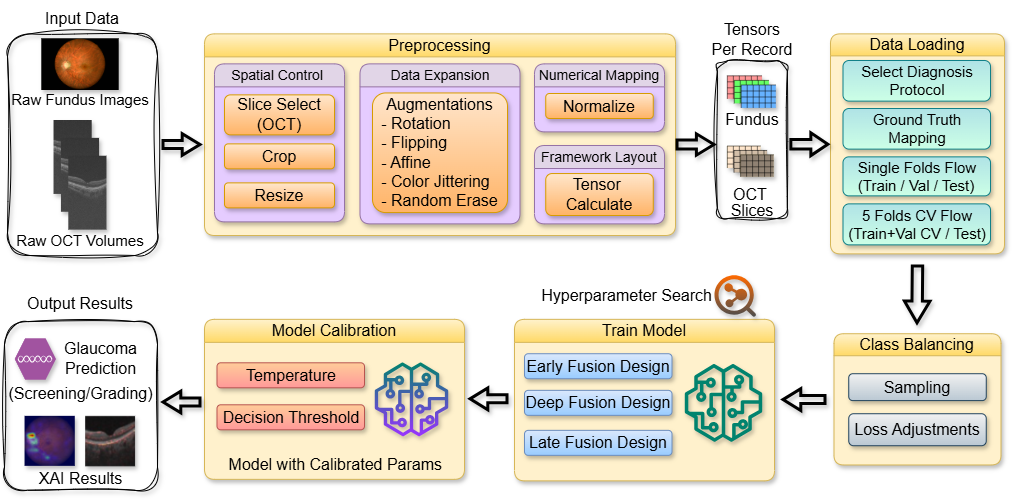
\includegraphics[width=\textwidth]{images/overall-process-diagram.png}
    \caption{Overall workflow of the proposed transformer-based multimodal framework for glaucoma screening and grading. Paired fundus photographs and OCT volumes undergo modality-specific preprocessing before being processed using Early, Deep, or Late Fusion. Model development includes task-specific training, hyperparameter optimization, calibration, evaluation, and post-hoc explainability analysis.}
    \label{fig:overall-workflow}
\end{figure*}

The workflow begins with paired fundus photographs and OCT volumes from the GAMMA dataset. Deterministic preprocessing includes quality inspection, region-of-interest extraction, OCT B-scan selection, spatial resizing, and modality-specific normalization. Stochastic training augmentations include horizontal flipping, mild rotation, affine transformation, fundus-specific color jittering, and random erasing. These transformations are applied only to training samples, while validation and test samples undergo deterministic preprocessing.

The original GAMMA labels are organized according to the target diagnostic task. For binary screening, early and mid-advanced glaucoma are merged into a single positive class, whereas the three original severity categories are retained for grading. The models are evaluated using both the official training--validation--test partition and a five-fold robustness protocol constructed from the combined official training and validation sets.

Three fusion architectures are investigated: Early Fusion at the input level, Deep Fusion at the latent representation level, and Late Fusion at the decision level. All three architectures use an OCT multiple-instance learning (OCT-MIL) mechanism to aggregate evidence from a selected subset of OCT B-scans. The architectures support transformer-family backbones, including Vision Transformer (ViT), Data-efficient Image Transformer (DeiT), Swin Transformer, and CoAtNet variants. Optional modules, including Feature-wise Linear Modulation (FiLM), modality-token attention, latent gating, and confidence-aware decision fusion, are treated as model-selection choices rather than being activated uniformly across all experiments.

Model configurations are selected through Optuna-based hyperparameter optimization. The search considers the backbone architecture, number of selected OCT slices, learning rate, weight decay, batch size, dropout, regularization, fine-tuning schedule, loss formulation, and fusion-specific modules. The full search space is provided in Supplementary Table~S1, while the configurations selected for the final models are reported with the experimental results. Following model training, temperature scaling and decision-rule selection are performed using validation data. The held-out official test set is used only for final evaluation and is not used for hyperparameter selection or calibration.

\subsection{Dataset and Task Formulation}
\label{subsec:dataset_tasks}

\subsubsection{GAMMA Dataset}
\label{subsubsec:gamma_dataset}

All experiments use the publicly available Glaucoma Grading from Multi-Modality Images (GAMMA) dataset, released as part of the MICCAI 2021 GAMMA Challenge~\cite{wu2023gamma}. The dataset contains paired color fundus photographs and three-dimensional OCT volumes acquired from the same eyes, making it suitable for evaluating multimodal glaucoma analysis.

The dataset comprises 300 paired samples distributed across predefined training, validation, and test sets containing 100 samples each. Each sample consists of a high-resolution color fundus photograph of $2992\times2000$ pixels, an OCT volume containing 256 grayscale B-scans of $512\times992$ pixels, and an expert-provided glaucoma severity label. The three diagnostic categories are normal, early glaucoma, and mid-advanced glaucoma.

The OCT volumes were acquired using a dense macula-centered scanning protocol covering a $3\times3$~mm region. Macular OCT imaging provides depth-resolved information related to retinal structures, including the RNFL and GCIPL. Although the dataset does not contain peripapillary OCT scans, the combination of macula-centered OCT and fundus photography provides complementary retinal-layer and optic-disc-related information for multimodal analysis.

Representative fundus and OCT inputs are shown in Figure~\ref{fig:raw-fundus-oct}. The fundus photograph provides global retinal, optic disc, and vascular context, whereas the OCT B-scan presents a cross-sectional view of retinal structures.

\begin{figure}[!t]
    \centering
    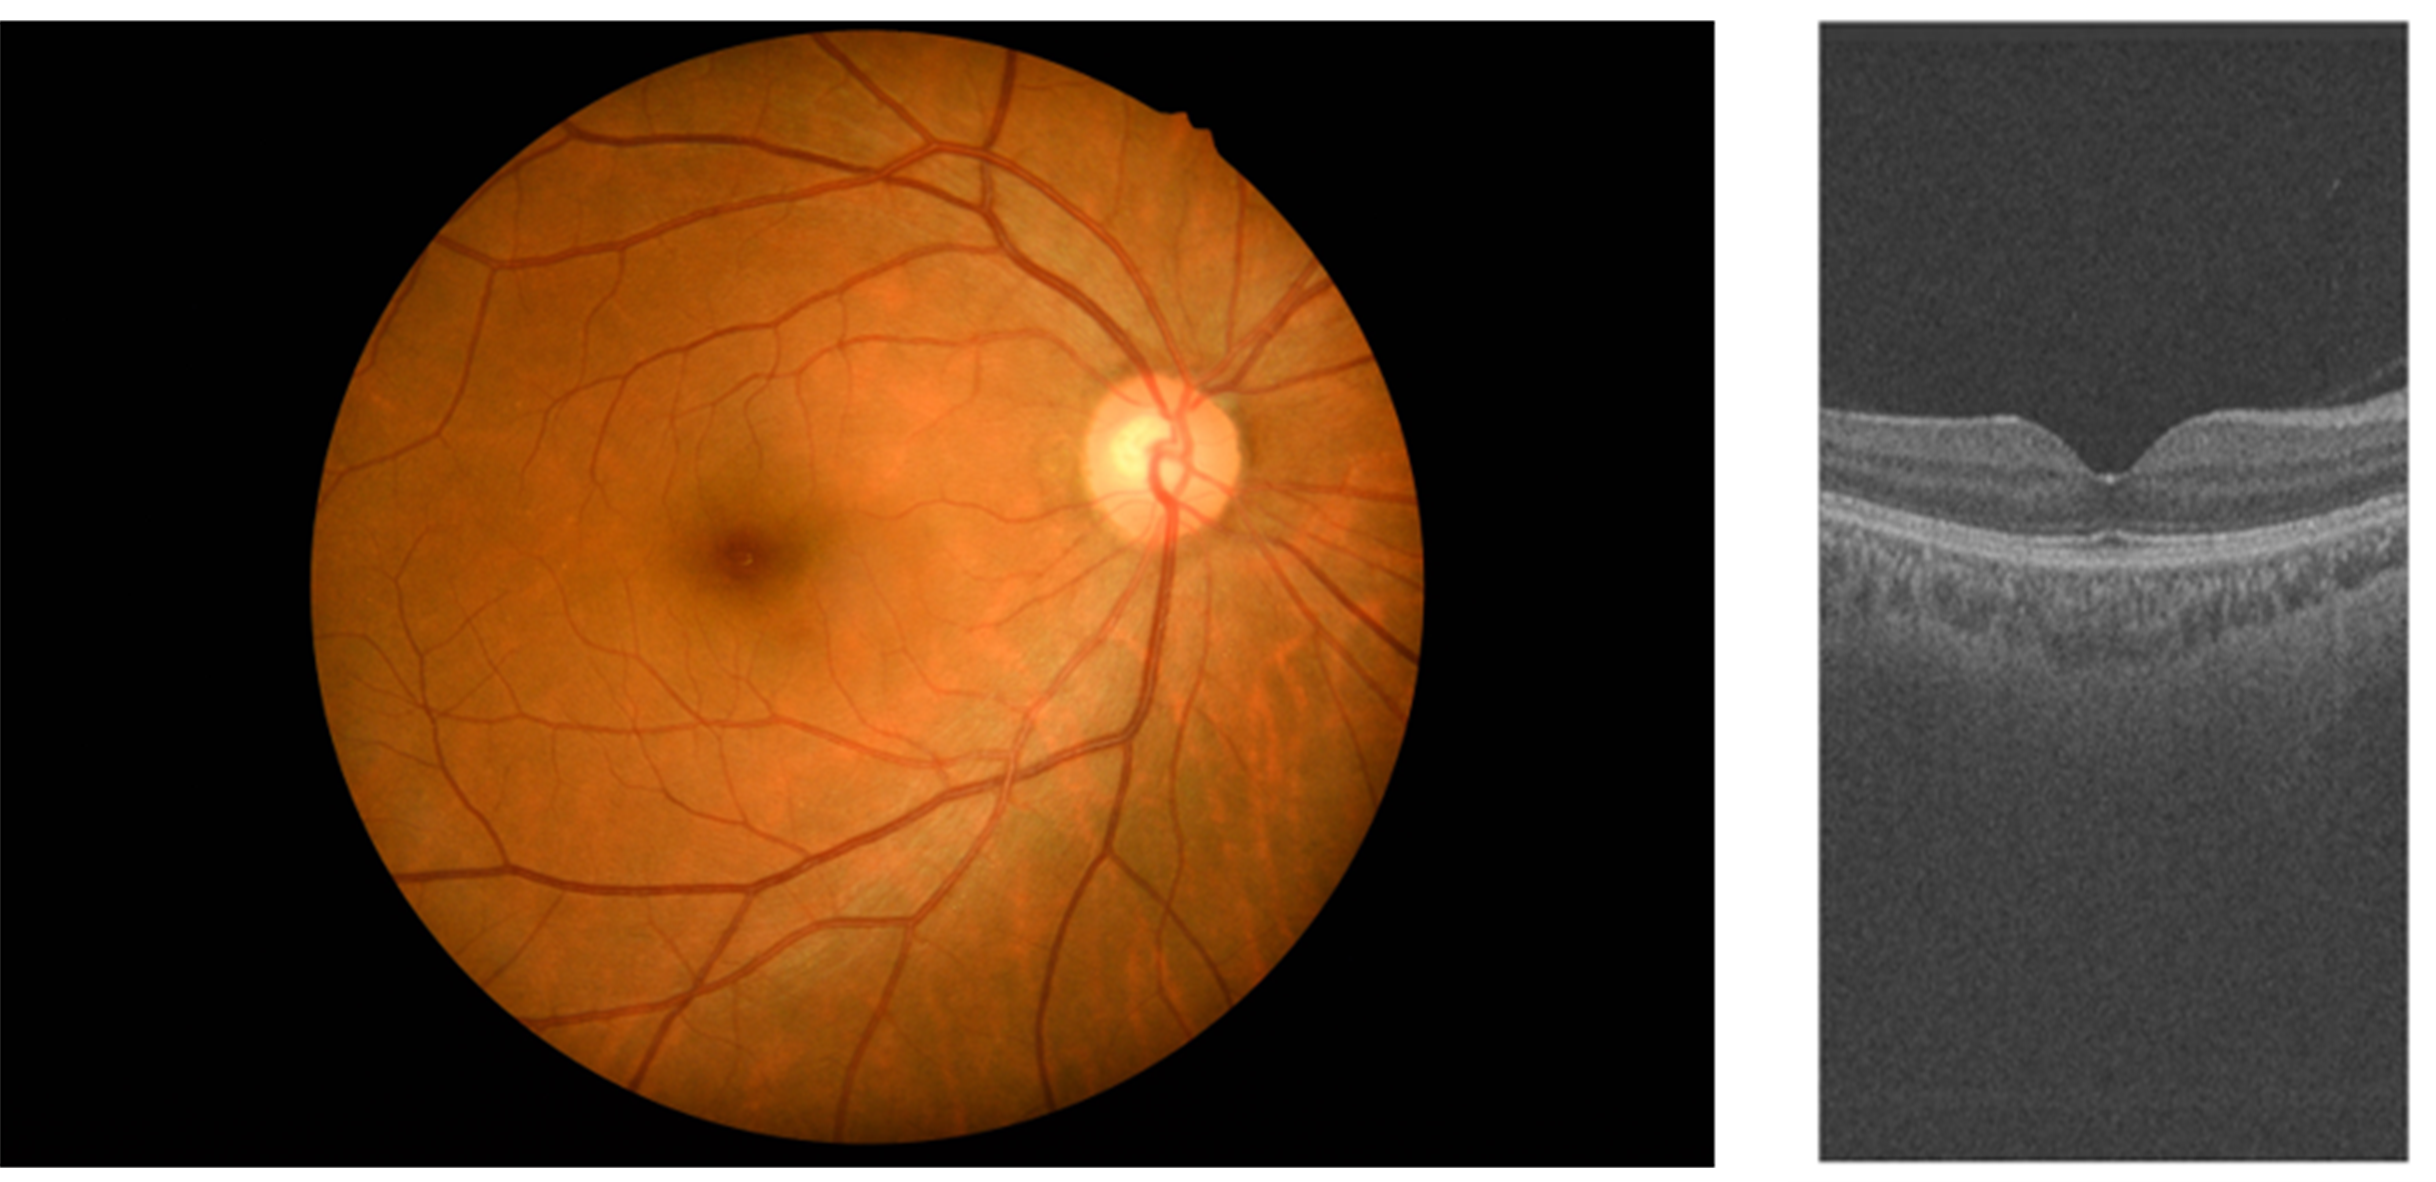
\includegraphics[width=\columnwidth]{images/raw-fundus-oct.png}
    \caption{Representative paired inputs from the GAMMA dataset: a color fundus photograph and a corresponding OCT B-scan.}
    \label{fig:raw-fundus-oct}
\end{figure}

Table~\ref{tab:dataset_summary} summarizes the class distributions used for binary screening and multiclass grading. No samples were excluded from the experiments.

\begin{table}[!t]
    \centering
    \caption{Class distributions for binary glaucoma screening and three-class glaucoma grading using the official GAMMA dataset splits.}
    \label{tab:dataset_summary}
    \small
    \setlength{\tabcolsep}{4pt}
    \begin{tabular}{lcccc}
        \hline
        \textbf{Task and class} &
        \textbf{Training}       &
        \textbf{Validation}     &
        \textbf{Test}           &
        \textbf{Total}                               \\
        \hline
        Screening: negative     & 50 & 50 & 51 & 151 \\
        Screening: positive     & 50 & 50 & 49 & 149 \\
        \hline
        Grading: normal         & 50 & 50 & 51 & 151 \\
        Grading: early          & 26 & 26 & 25 & 77  \\
        Grading: mid-advanced   & 24 & 24 & 24 & 72  \\
        \hline
    \end{tabular}
\end{table}

\subsubsection{Binary Glaucoma Screening}
\label{subsubsec:binary_screening}

For binary glaucoma screening, the original severity labels are mapped into glaucomatous and non-glaucomatous categories. Normal samples are assigned to the negative class, while early and mid-advanced glaucoma samples are combined into the positive class. This formulation represents a referral-oriented screening objective in which eyes showing any labelled glaucoma severity are separated from normal eyes.

The resulting binary dataset is approximately balanced, comprising 151 negative and 149 positive samples. Consequently, conventional mini-batch sampling is used as the default for screening, while sensitivity, specificity, AUC-ROC, and AUC-PR are included to characterize discrimination across clinically relevant operating conditions.

\subsubsection{Multiclass Glaucoma Grading}
\label{subsubsec:multiclass_grading}

For glaucoma grading, the original GAMMA labels are retained, producing a three-class problem consisting of normal, early glaucoma, and mid-advanced glaucoma. The classes are ordinal because misclassification between distant severity categories is more consequential than confusion between adjacent categories.

The grading data are imbalanced, with normal samples accounting for approximately half of each official split. This imbalance motivates the evaluation of sampling- and loss-level correction strategies during model selection. Quadratically weighted Cohen's kappa (QWK) is used as the primary grading metric because it accounts for both chance agreement and the ordinal distance between the true and predicted classes. Accuracy and macro-averaged F1-score are used as complementary measures.

\subsection{Multimodal Image Preprocessing}
\label{subsec:preprocessing}

Consistent preprocessing is important for stable optimization and reproducible evaluation of multimodal medical image models~\cite{virbukaite2023impact,sun2025hybrid}. The proposed pipeline applies modality-specific operations to preserve diagnostically relevant fundus and OCT information while reducing non-informative background and computational overhead. Deterministic preprocessing is performed offline and cached, whereas stochastic augmentation and final tensor normalization are performed online during training.

Detailed pseudocode for fundus field-of-view extraction, OCT region-of-interest selection, and foveal-center estimation is provided in Supplementary Algorithms~S1--S3.

\subsubsection{Fundus Image Preprocessing}
\label{subsubsec:fundus_preprocessing}

Each fundus photograph is first converted to grayscale for field-of-view detection. A binary foreground mask is generated using an intensity threshold, after which the largest external contour is identified as the retinal field. A square region centered on the contour centroid is extracted using the maximum dimension of its bounding box. This procedure removes non-informative black borders while preserving the complete retinal field rather than restricting the input to a manually localized optic-disc crop.

Retaining the complete retinal field allows the model to use both optic-disc-related evidence and wider contextual information, including parapapillary and vascular patterns. If the retinal contour cannot be identified, the original image is resized without cropping as a deterministic fallback. The extracted region is resized to $224\times224$ pixels to match the standard input size of the pretrained backbone candidates.

\subsubsection{OCT Preprocessing and Slice Selection}
\label{subsubsec:oct_preprocessing}

Each GAMMA OCT volume contains 256 B-scans. Processing the complete volume with a dense three-dimensional model would create a high-dimensional learning problem relative to the 300 available paired samples. The framework therefore selects a compact subset of B-scans and aggregates their diagnostic evidence through OCT-MIL.

The candidate B-scans are selected from a symmetric window centered on an automatically estimated foveal slice. Foveal-center estimation is based on the vitreous--retina interface, with the selected center corresponding to the candidate slice exhibiting the maximum estimated interface arc length within a local search region. The candidate slice counts are treated as hyperparameters, enabling model selection to balance anatomical coverage, computational cost, and validation performance. The investigated slice counts are reported in Supplementary Table~S1.

For each selected B-scan, a weighted gradient-based procedure identifies a square high-information region containing prominent retinal-layer boundaries. The method applies denoising, estimates image-gradient magnitude, and evaluates candidate square windows along the longer image dimension using a center-weighted gradient score. The highest-scoring region is extracted and resized to $224\times224$ pixels. This reduces background content and limits the geometric distortion that would otherwise result from directly resizing the complete non-square B-scan.

\subsubsection{Data Augmentation and Normalization}
\label{subsubsec:augmentation_normalization}

Stochastic augmentation is applied only to the training data. The augmentation pipeline includes horizontal flipping, mild rotation, affine transformation, color jittering for fundus photographs, and random erasing for both modalities. The transformation ranges are constrained to avoid severe deformations that would alter retinal anatomy. Because the fundus photograph and selected OCT B-scans represent different anatomical views rather than registered pixel-level views, modality-appropriate augmentations are applied without assuming direct spatial correspondence between their pixels.

Fundus photographs are normalized using ImageNet channel-wise statistics to remain compatible with ImageNet-pretrained model initialization. OCT B-scans are normalized using z-score normalization based on training-data intensity statistics. Validation and test samples undergo only deterministic cropping, resizing, and normalization, without stochastic augmentation.

The offline stage performs computationally intensive deterministic operations, including fundus cropping, OCT slice selection, OCT region extraction, and resizing. The resulting images are cached to reduce repeated CPU processing. The online data loader subsequently performs stochastic augmentation, channel conversion, normalization, and tensor construction. This separation ensures consistent anatomical framing across fusion strategies while reducing training overhead.

\subsection{Transformer-Based Multimodal Fusion Framework}
\label{subsec:fusion_framework}

The proposed framework evaluates three levels of multimodal interaction: input-level Early Fusion, latent-level Deep Fusion, and decision-level Late Fusion. Each strategy receives the same paired fundus and OCT information and uses the shared OCT-MIL principle described below. The primary difference is the stage at which information from the two modalities is combined.

The architectures are designed to support multiple compact transformer-family backbones, including ViT, DeiT, Swin Transformer, and CoAtNet. ImageNet-pretrained weights are used where available. The final classifier produces one logit for binary screening or three logits for glaucoma grading.

\subsubsection{OCT Multiple-Instance Learning}
\label{subsubsec:oct_mil}

An OCT volume is represented as a collection of selected B-scans rather than as a single dense three-dimensional tensor. Each selected OCT B-scan is therefore treated as an instance belonging to one eye-level bag. A shared OCT slice encoder maps the $s$th B-scan of sample $i$ to an embedding $\mathbf{e}_{i,s}^{O}$. Because pretrained image encoders expect three-channel inputs, each grayscale OCT slice is duplicated across three channels before encoding.

The diagnostic relevance of each slice is estimated using a trainable attention mechanism:

\begin{equation}
    a_{i,s} =
    \frac{
        \exp\!\left(
        \mathbf{v}^{\top}
        \sigma\!\left(\mathbf{W}\mathbf{e}_{i,s}^{O}\right)
        \right)
    }{
        \sum_{t=1}^{S}
        \exp\!\left(
        \mathbf{v}^{\top}
        \sigma\!\left(\mathbf{W}\mathbf{e}_{i,t}^{O}\right)
        \right)
    },
    \qquad
    \sum_{s=1}^{S}a_{i,s}=1,
    \label{eq:mil_attention}
\end{equation}

where $\mathbf{W}$ and $\mathbf{v}$ are trainable parameters, $\sigma(\cdot)$ denotes a nonlinear activation, and $S$ is the selected number of B-scans. For Deep and Late Fusion, the eye-level OCT embedding is computed as

\begin{equation}
    \mathbf{e}_{i}^{O}
    =
    \sum_{s=1}^{S}
    a_{i,s}\mathbf{e}_{i,s}^{O}.
    \label{eq:mil_embedding}
\end{equation}

For Early Fusion, the attention values are instead used to construct an attention-weighted spatial OCT summary:

\begin{equation}
    \mathbf{O}_{i}^{\mathrm{agg}}(p,q)
    =
    \sum_{s=1}^{S}
    a_{i,s}\mathbf{O}_{i,s}(p,q),
    \label{eq:mil_spatial}
\end{equation}

where $\mathbf{O}_{i,s}(p,q)$ denotes the intensity at spatial location $(p,q)$ in the preprocessed $s$th B-scan. OCT-MIL reduces the dimensionality of the volume while preserving a learnable estimate of inter-slice relevance. The learned attention values are also used during post-hoc explainability analysis to identify the B-scans contributing most strongly to each prediction.

\subsubsection{Early Fusion}
\label{subsubsec:early_fusion}

Early Fusion combines fundus and OCT information before high-level feature extraction. The architecture is shown in Figure~\ref{early-fusion-architecture}. For sample $i$, let the preprocessed fundus photograph be $\mathbf{F}_{i}\in\mathbb{R}^{3\times H\times W}$ and the attention-weighted OCT summary produced by Equation~\eqref{eq:mil_spatial} be $\mathbf{O}_{i}^{\mathrm{agg}}\in\mathbb{R}^{1\times H\times W}$.

\begin{figure*}[!t]
    \centering
    \includegraphics[width=\textwidth]{images/early-fusion-architecture.png}
    \caption{Early Fusion architecture. Selected OCT B-scans are aggregated using OCT-MIL, concatenated with the fundus photograph at the input level, and processed by a shared transformer-family encoder. FiLM modulation is included as an optional model-selection component.}
    \label{early-fusion-architecture}
\end{figure*}

The two inputs are concatenated channel-wise to form

\begin{equation}
    \mathbf{X}_{i}
    =
    \left[
    \mathbf{F}_{i}
    \,\|\,
    \mathbf{O}_{i}^{\mathrm{agg}}
    \right]
    \in\mathbb{R}^{4\times H\times W}.
    \label{eq:early_concat}
\end{equation}

A $1\times1$ convolutional adapter followed by normalization projects the four-channel input into a three-channel representation compatible with the pretrained image encoders:

\begin{equation}
    \hat{\mathbf{X}}_{i}
    =
    \mathcal{A}\!\left(\mathbf{X}_{i}\right)
    \in\mathbb{R}^{3\times H\times W}.
    \label{eq:early_adapter}
\end{equation}

An optional FiLM module is used to recalibrate the adapted multimodal representation using learned channel-wise scale and shift parameters~\cite{perez2018film}. The bounded modulation is expressed as

\begin{equation}
    \hat{\mathbf{X}}_{i}^{\mathrm{film}}(k,p,q)
    =
    \left(1+0.1\tanh(\gamma_{i,k})\right)
    \hat{\mathbf{X}}_{i}(k,p,q)
    +
    0.1\tanh(\beta_{i,k}),
    \label{eq:early_film}
\end{equation}

where $\gamma_{i,k}$ and $\beta_{i,k}$ are generated from a global descriptor of the multimodal input. Bounding the modulation causes the module to behave near an identity transformation at initialization and reduces unstable changes to pretrained input representations. The inclusion of FiLM is determined through validation-based hyperparameter selection rather than being fixed across all tasks.

The adapted input is processed by a shared transformer-family encoder to obtain a multimodal representation $\mathbf{z}_{i}$. A regularized multilayer classifier maps this representation to either one screening logit or a three-dimensional grading logit vector. Early Fusion permits shared representation learning from the beginning of the network, but it also requires a single encoder to process fundus and OCT information with substantially different visual characteristics.

\subsubsection{Deep Fusion}
\label{subsubsec:deep_fusion}

Deep Fusion preserves modality-specific feature extraction and combines fundus and OCT representations in a shared latent space. As illustrated in Figure~\ref{deep-fusion-architecture}, the fundus photograph and selected OCT slices are passed through separate encoders before multimodal integration.

\begin{figure*}[!t]
    \centering
    \includegraphics[width=\textwidth]{images/deep-fusion-architecture.png}
    \caption{Deep Fusion architecture. Fundus and OCT information are encoded independently and integrated at the latent representation level. Modality-token attention and gated feature rebalancing are optional components selected according to validation performance.}
    \label{deep-fusion-architecture}
\end{figure*}

The fundus encoder produces

\begin{equation}
    \mathbf{e}_{i}^{F}
    =
    \operatorname{Enc}_{F}\!\left(\mathbf{F}_{i}\right)
    \in \mathbb{R}^{D_F},
    \label{eq:fundus_encoder}
\end{equation}

while the shared OCT slice encoder and OCT-MIL module produce the eye-level OCT representation $\mathbf{e}_{i}^{O}\in\mathbb{R}^{D_O}$ according to Equations~\eqref{eq:mil_attention} and~\eqref{eq:mil_embedding}. The fundus and OCT embeddings are projected into a common $D$-dimensional latent space:

\begin{equation}
    \tilde{\mathbf{e}}_{i}^{F}
    =
    \mathbf{P}_{F}\mathbf{e}_{i}^{F},
    \qquad
    \tilde{\mathbf{e}}_{i}^{O}
    =
    \mathbf{P}_{O}\mathbf{e}_{i}^{O},
    \label{eq:deep_projection}
\end{equation}

where $\mathbf{P}_{F}$ and $\mathbf{P}_{O}$ are learned projection matrices.

The base Deep Fusion representation is produced by concatenating the projected modality embeddings and mapping them into a compact shared representation:

\begin{equation}
    \mathbf{h}_{i}
    =
    \sigma\!\left(
    \mathbf{W}_{f}
    \left[
        \tilde{\mathbf{e}}_{i}^{F};
        \tilde{\mathbf{e}}_{i}^{O}
        \right]
    +
    \mathbf{b}_{f}
    \right),
    \label{eq:deep_concat}
\end{equation}

where $\sigma(\cdot)$ denotes a nonlinear activation. This formulation enables modality-specific representation learning while permitting direct interaction between fundus and OCT information before classification.

An optional modality-token interaction module may be applied to increase cross-modal interaction. A learnable classification token is combined with the projected fundus and OCT embeddings to form

\begin{equation}
    \mathbf{T}_{i}
    =
    \left[
        \mathbf{c}_{0}
        \,\|\,
        \tilde{\mathbf{e}}_{i}^{F}
        \,\|\,
        \tilde{\mathbf{e}}_{i}^{O}
        \right]
    \in\mathbb{R}^{3\times D}.
    \label{eq:deep_tokens}
\end{equation}

Multi-head self-attention is then applied to the short modality-token sequence:

\begin{equation}
    \hat{\mathbf{T}}_{i}
    =
    \operatorname{MHA}
    \left(
    \mathbf{T}_{i},
    \mathbf{T}_{i},
    \mathbf{T}_{i}
    \right),
    \qquad
    \mathbf{h}_{i}
    =
    \hat{\mathbf{T}}_{i}[0].
    \label{eq:deep_attention}
\end{equation}

Although this component facilitates cross-modal exchange, it is implemented as self-attention over a compact modality-token sequence rather than as dense attention between all fundus and OCT image tokens. This limits its computational and parameter overhead.

An optional gating module may further reweight the fused representation using information from both modalities~\cite{song2022cross}:

\begin{equation}
    \mathbf{g}_{i}
    =
    \operatorname{sigmoid}
    \left(
    \mathbf{W}_{g}
    \left[
        \tilde{\mathbf{e}}_{i}^{F};
        \tilde{\mathbf{e}}_{i}^{O}
        \right]
    +
    \mathbf{b}_{g}
    \right),
    \qquad
    \mathbf{h}_{i}^{\prime}
    =
    \mathbf{g}_{i}\odot\mathbf{h}_{i}.
    \label{eq:deep_gate}
\end{equation}

The inclusion of modality-token attention and gated rebalancing is treated as a validation-based model-selection choice. Consequently, the selected screening and grading models may use different Deep Fusion variants if additional interaction modules do not improve validation performance for both tasks. This maintains a common latent-fusion principle while avoiding unnecessary complexity under the limited-data setting.

The resulting representation is passed through a regularized classifier:

\begin{equation}
    \hat{\mathbf{y}}_{i}
    =
    \mathbf{W}_{c}
    \operatorname{Dropout}
    \left(
    \sigma\!\left(
        \mathbf{W}_{h}\mathbf{h}_{i}^{\prime}
        +
        \mathbf{b}_{h}
        \right)
    \right)
    +
    \mathbf{b}_{c},
    \label{eq:deep_classifier}
\end{equation}

where $\hat{\mathbf{y}}_{i}$ contains one logit for screening or three logits for grading. When gating is not selected, $\mathbf{h}_{i}^{\prime}$ is replaced by the ungated fused representation $\mathbf{h}_{i}$.

\subsubsection{Late Fusion}
\label{subsubsec:late_fusion}

Late Fusion combines modality-specific predictions at the decision level. As shown in Figure~\ref{late-fusion-architecture}, the fundus and OCT branches are trained to generate separate task-specific logits before their outputs are combined.

\begin{figure*}[!t]
    \centering
    \includegraphics[width=\textwidth]{images/late-fusion-architecture.png}
    \caption{Late Fusion architecture. Fundus and OCT branches generate independent predictions that are combined using optional modality-specific temperature calibration and confidence-aware logit weighting.}
    \label{late-fusion-architecture}
\end{figure*}

The fundus encoder and OCT-MIL branch produce modality-specific representations $\mathbf{e}_{i}^{F}$ and $\mathbf{e}_{i}^{O}$. Separate classifier heads map these representations to logits:

\begin{equation}
    \boldsymbol{\ell}_{i}^{F}
    =
    \operatorname{Head}_{F}\!\left(\mathbf{e}_{i}^{F}\right),
    \qquad
    \boldsymbol{\ell}_{i}^{O}
    =
    \operatorname{Head}_{O}\!\left(\mathbf{e}_{i}^{O}\right).
    \label{eq:late_logits}
\end{equation}

The logits are scalar-valued for binary screening and three-dimensional for grading. Optional modality-specific temperature scaling is applied before fusion:

\begin{equation}
    \tilde{\boldsymbol{\ell}}_{i}^{F}
    =
    \frac{\boldsymbol{\ell}_{i}^{F}}{\tau_{F}},
    \qquad
    \tilde{\boldsymbol{\ell}}_{i}^{O}
    =
    \frac{\boldsymbol{\ell}_{i}^{O}}{\tau_{O}},
    \qquad
    \tau_F,\tau_O>0.
    \label{eq:late_temperature}
\end{equation}

The modality-specific temperatures in Equation~\eqref{eq:late_temperature} are internal components of Late Fusion and are distinct from the post-hoc calibration of the final fused output described in Section~\ref{subsec:calibration_inference}.

When confidence-aware fusion is enabled, a lightweight network estimates normalized sample-specific modality weights:

\begin{equation}
    \left[
        c_{i}^{F},
        c_{i}^{O}
        \right]
    =
    \operatorname{Softmax}
    \left(
    \operatorname{MLP}
    \left(
        \mathbf{r}_{i}
        \right)
    \right),
    \qquad
    c_{i}^{F}+c_{i}^{O}=1,
    \label{eq:late_confidence}
\end{equation}

where $\mathbf{r}_{i}$ contains summary statistics derived from the fundus and OCT logits. The final fused logits are

\begin{equation}
    \hat{\boldsymbol{\ell}}_{i}
    =
    c_{i}^{F}\tilde{\boldsymbol{\ell}}_{i}^{F}
    +
    c_{i}^{O}\tilde{\boldsymbol{\ell}}_{i}^{O}.
    \label{eq:late_fusion}
\end{equation}

When modality-specific calibration and confidence weighting are not selected, $\tau_F=\tau_O=1$ and $c_i^F=c_i^O=0.5$, reducing Equation~\eqref{eq:late_fusion} to arithmetic mean-logit fusion. The inclusion of modality-specific temperature scaling and confidence-aware weighting is determined through validation-based hyperparameter selection. This enables comparison between simple and adaptive decision-level integration without changing the independent modality branches.

\subsection{Model Training and Hyperparameter Optimization}
\label{subsec:model_training}

All fusion models are trained independently for binary screening and multiclass grading. The general optimization pipeline is shared across tasks, while the loss functions, sampling strategies, output dimensions, and model-selection objectives are adapted to the corresponding diagnostic problem.

\subsubsection{Optimization and Regularization}
\label{subsubsec:optimization}

ImageNet-pretrained weights are used to initialize the transformer-family encoders where available. Newly introduced projection layers, adapters, fusion modules, and classifier heads are initialized independently and trained for the target task. Training is performed using the AdamW optimizer with separate learning-rate multipliers for pretrained backbones and newly initialized layers.

The optimization schedule includes linear learning-rate warm-up, validation-based early stopping, and optional staged backbone freezing and unfreezing. Differential learning rates allow the pretrained encoders to be updated more conservatively than the fusion and classification modules. Dropout, weight decay, data augmentation, and gradient clipping are used to reduce overfitting and optimization instability. Exponential moving average or stochastic weight averaging is included among the candidate training options for grading and is retained only when selected by validation performance.

The number of OCT B-scans is also optimized rather than fixed across all models. This permits each architecture to balance OCT coverage against computational cost and overfitting risk. The selected number of slices, backbone, regularization settings, and fusion-module configuration for each final model are reported in the Results section.

\subsubsection{Task-Specific Loss Functions}
\label{subsubsec:loss_functions}

Binary glaucoma screening is optimized using label-smoothed binary cross-entropy. For sample $i$, the smoothed binary target is

\begin{equation}
    \tilde{y}_{i}
    =
    (1-\epsilon)y_{i}
    +
    0.5\epsilon,
    \label{eq:binary_smoothing}
\end{equation}

where $y_i\in\{0,1\}$ and $\epsilon$ is the smoothing coefficient. Given the predicted screening logit $\hat{y}_{i}$, the loss is

\begin{equation}
    \mathcal{L}_{\mathrm{bin}}
    =
    -\frac{1}{N}
    \sum_{i=1}^{N}
    \left[
        \tilde{y}_{i}\log\sigma(\hat{y}_{i})
        +
        \left(1-\tilde{y}_{i}\right)
        \log\left(1-\sigma(\hat{y}_{i})\right)
        \right].
    \label{eq:binary_loss}
\end{equation}

The smoothing coefficient is reduced during training, allowing stronger regularization during early optimization while permitting sharper decision boundaries during later epochs.

For multiclass grading, the model-selection process evaluates candidate imbalance-aware objectives. The final grading models use focal loss because it provided the selected validation behavior under the imbalanced class distribution. For $C=3$ classes, focal loss is defined as

\begin{equation}
    \mathcal{L}_{\mathrm{focal}}
    =
    -\frac{1}{N}
    \sum_{i=1}^{N}
    \sum_{c=1}^{C}
    \alpha_c
    \left(1-p_{i,c}\right)^{\gamma}
    y_{i,c}\log(p_{i,c}),
    \label{eq:focal_loss}
\end{equation}

where $p_{i,c}$ is the predicted Softmax probability for class $c$, $y_{i,c}$ is the one-hot target, $\gamma$ controls the emphasis placed on difficult samples, and $\alpha_c$ represents the class-specific weight. The class weights are constrained during optimization to avoid excessive weighting of minority classes.

Weighted random sampling is included as an optional grading strategy. When activated, sample probabilities are derived from inverse class frequencies with smoothing to limit repeated oversampling of minority-class observations. The combination of loss formulation and sampling strategy is selected using validation data.

\subsubsection{Hyperparameter Optimization}
\label{subsubsec:hyperparameter_optimization}

Hyperparameter optimization is conducted separately for each fusion strategy and diagnostic task using the Optuna framework. For binary glaucoma screening, 50 trials are conducted for each of the Early, Deep, and Late Fusion architectures, resulting in a total of 150 screening trials. For multiclass glaucoma grading, 100 trials are conducted for each fusion architecture, resulting in a total of 300 grading trials. Screening trials are ranked primarily according to validation AUC-ROC. Grading trials are optimized using validation loss, while QWK and macro-F1 are additionally monitored to ensure that model selection is not driven solely by the majority class.

The search space includes the learning rate, weight decay, batch size, backbone architecture, number of OCT B-scans, transformer and classifier dropout, label smoothing, warm-up duration, backbone freezing schedule, fine-tuning learning rate, MIL attention temperature, sampling strategy, grading-loss type, focal-loss parameters, and architecture-specific optional modules. The complete search space is provided in Supplementary Table~S1. The final selected configuration for each fusion strategy is reported in the Results section to connect model configuration with observed performance.

All model selection is performed using the corresponding validation data. The official test labels are not used to choose hyperparameters, optional modules, calibration temperatures, classification thresholds, or training duration.

\subsection{Calibration and Inference}
\label{subsec:calibration_inference}

Following supervised training, post-hoc temperature scaling is optionally applied to the final output of each Early, Deep, and Late Fusion model. Its inclusion is determined as part of the validation-based configuration process. This final-output calibration is distinct from the modality-specific temperature scaling used internally by the Late Fusion architecture.

Given a final model-logit vector $\mathbf{z}_{i}$, the calibrated probabilities are computed as

\begin{equation}
    \mathbf{p}_{i}^{\mathrm{cal}}
    =
    \operatorname{Softmax}
    \left(
    \frac{\mathbf{z}_{i}}{\tau}
    \right),
    \qquad
    \tau>0,
    \label{eq:posthoc_temperature}
\end{equation}

where the scalar temperature $\tau$ is estimated using the validation predictions by minimizing cross-entropy loss. For binary classification, the model output is treated as the corresponding two-class probability formulation. Temperature scaling adjusts the sharpness of the predicted probability distribution without changing the ordering of the output logits.

For screening, a decision threshold is selected using the validation data by maximizing Youden's $J$ statistic:

\begin{equation}
    J(t)
    =
    \operatorname{Sensitivity}(t)
    +
    \operatorname{Specificity}(t)
    -1.
    \label{eq:youden}
\end{equation}

The resulting threshold is fixed before evaluation on the official test set.

For glaucoma grading, calibrated class probabilities are interpreted using class-specific confidence thresholds determined exclusively from the validation data. The class with the highest calibrated probability is selected when its corresponding confidence threshold is satisfied. For low-confidence cases in which this threshold is not satisfied, the two classes with the highest calibrated probabilities are considered and the higher-severity class is selected. This ordinal decision rule was fixed using validation data before evaluation of the official test predictions.

At inference time, the selected model checkpoint is loaded together with its preprocessing configuration, selected OCT slice count, calibration parameters, and decision thresholds. Test samples undergo the same deterministic preprocessing used for validation, without random augmentation. Test-time augmentation is applied to every glaucoma grading model using the predefined deterministic transformations. The resulting probability vectors are averaged before post-hoc calibration and application of the validation-derived grading decision rule. Test-time augmentation is not applied to the binary screening models unless otherwise specified.

\subsection{Evaluation Protocol and Statistical Analysis}
\label{subsec:evaluation_protocol}

\subsubsection{Official Dataset Split}
\label{subsubsec:official_split}

The primary experiments use the official GAMMA training, validation, and test sets. Models are fitted using the 100-sample training split, while the 100-sample validation split is used for early stopping, hyperparameter selection, optional-module selection, calibration, and decision-threshold estimation. The selected configuration is evaluated on the held-out 100-sample official test set.

The official test set is not used during model optimization or configuration selection. Results from this protocol provide the primary comparison among Early, Deep, and Late Fusion and permit comparison with other GAMMA-based studies that use the official data partition.

\subsubsection{Cross-Validation and Bootstrap Analysis}
\label{subsubsec:robustness_analysis}

A five-fold robustness analysis is conducted by combining the official training and validation sets, producing a development cohort of 200 paired samples. Stratified five-fold partitioning is then applied while preserving the corresponding binary or multiclass distribution. In each iteration, four folds are used for model fitting and the remaining fold is used as the internal validation set for checkpoint selection and calibration.

Each of the five resulting fold-specific models is subsequently evaluated once on the unchanged official 100-sample test set. The cross-validation results reported in this study are the mean and standard deviation of the official-test metrics obtained from these five independently trained fold models. Thus, the reported cross-validation variability reflects the sensitivity of test performance to different development-set partitions rather than the average of the five internal validation-fold scores.

For glaucoma grading, bootstrap resampling is additionally performed using the final official-test predictions to quantify statistical uncertainty. Test observations and their corresponding predictions are sampled with replacement using 1,000 bootstrap replicates. QWK, accuracy, and macro-averaged performance measures are recalculated for each replicate, and the resulting empirical distributions are used to estimate 95\% confidence intervals. This analysis quantifies uncertainty in the reported test-set performance without retraining the models.

\subsubsection{Evaluation Metrics}
\label{subsubsec:evaluation_metrics}

Binary screening performance is evaluated using AUC-ROC, AUC-PR, accuracy, sensitivity, specificity, precision, F1-score, and Brier score. AUC-ROC measures ranking performance across decision thresholds, while AUC-PR is included because it emphasizes positive-class retrieval. Sensitivity and specificity characterize performance at the validation-selected operating threshold.

The Brier score evaluates the squared error of predicted probabilities:

\begin{equation}
    \operatorname{Brier}
    =
    \frac{1}{N}
    \sum_{i=1}^{N}
    \left(
    \hat{p}_{i}-y_{i}
    \right)^2,
    \label{eq:brier_score}
\end{equation}

where $\hat{p}_{i}$ is the calibrated probability of glaucoma and $y_i$ is the binary target.

For multiclass grading, QWK is the primary metric because the target categories have an ordinal interpretation. It is defined as

\begin{equation}
    \kappa_{w}
    =
    1-
    \frac{
    \sum_{i,j}w_{ij}O_{ij}
    }{
    \sum_{i,j}w_{ij}E_{ij}
    },
    \label{eq:qwk_metric}
\end{equation}

where $O_{ij}$ and $E_{ij}$ are the observed and expected agreement matrices and $w_{ij}$ contains quadratic disagreement weights. Accuracy, macro-F1, weighted-F1, class-wise precision, recall, and one-vs-rest AUC are used as complementary measures. Macro-F1 is included to prevent the majority normal class from dominating the reported grading performance.

\subsection{Explainability Analysis}
\label{subsec:explainability}

Post-hoc explainability analysis is conducted using Grad-CAM and the attention values generated by OCT-MIL. The analysis is intended to support qualitative examination of image regions associated with model predictions and is not treated as evidence of causal or clinically validated reasoning.

For fundus photographs, Grad-CAM is applied to a late-stage feature-producing block of the selected backbone. For target class $c$, the importance of feature channel $k$ is calculated by spatially averaging the gradient of the class score $y^{c}$ with respect to activation map $\mathbf{A}^{k}$:

\begin{equation}
    \alpha_{k}^{c}
    =
    \frac{1}{Z}
    \sum_{p,q}
    \frac{\partial y^{c}}
    {\partial A_{p,q}^{k}},
    \label{eq:gradcam_weights}
\end{equation}

where $Z$ is the number of spatial positions. The class activation map is computed as

\begin{equation}
    \mathbf{L}_{\mathrm{Grad\text{-}CAM}}^{c}
    =
    \operatorname{ReLU}
    \left(
    \sum_{k}
    \alpha_{k}^{c}\mathbf{A}^{k}
    \right).
    \label{eq:gradcam_map}
\end{equation}

The resulting map is resized and overlaid on the fundus photograph to visualize the retinal regions most strongly associated with the selected class score.

OCT explanations are generated in two stages. First, the MIL attention values from Equation~\eqref{eq:mil_attention} are used to rank the selected B-scans according to their contribution to the eye-level OCT representation. Second, Grad-CAM is applied to the highest-attention B-scans to identify salient locations within the selected slices. This combination provides both inter-slice importance and intra-slice localization for the OCT modality.

A lightweight web-based research interface, termed \textit{MultiGlaucoFormer}, was also developed to demonstrate paired-input inference and the corresponding fundus and OCT explanation maps~\cite{multiglaucoformer_webapp}. Because the interface has not undergone prospective or clinical validation, its implementation details and graphical user interface are provided in the Supplementary Material and it is not considered part of the clinical evaluation.



\section{RESULTS ANALYSIS AND DISCUSSION}
\label{sec4}

All results reported in this section are obtained under a unified experimental framework, where data preprocessing, backbone selection, optimization strategy, and evaluation protocols are kept consistent across fusion strategies. This design enables direct and controlled comparison of Early, Deep, and Late Fusion multimodal fusion mechanisms for both glaucoma screening and glaucoma grading, isolating the effect of fusion granularity and task-aligned architectural choices.

\subsection{Fairness of Experimental Comparison}
\label{subsec:fairness_protocol}

To ensure that performance differences reflect fusion behaviour rather than confounding experimental settings, all fusion strategies are evaluated under the same dataset splits, deterministic preprocessing pipeline, image resolution, augmentation policy, optimizer family, calibration procedure, and task-specific evaluation metrics. Hyperparameter optimization is conducted independently for each fusion strategy because the optimal learning rate, regularization strength, backbone selection, and OCT slice count may differ across fusion depths. However, the search space is kept consistent across strategies within each diagnostic protocol. Unimodal baselines and ablation variants use the same preprocessing, loss formulation, and evaluation protocol as their corresponding multimodal models. This controlled setup allows the effects of Early, Deep, and Late Fusion to be compared more fairly than comparisons across independently designed pipelines.

\subsection{Hyperparameter Optimization Outcomes}
\label{subsec:hpo-results}

Hyperparameter optimization was conducted independently for each fusion strategy to ensure fair comparison and stable convergence under both diagnostic protocols. Bayesian optimization using the Optuna framework was employed, with the objective of maximizing validation performance while controlling overfitting on the limited dataset.

For the \emph{binary glaucoma screening} protocol, 50 optimization trials were executed per fusion strategy, resulting in a total of 150 trained models (Early, Deep, and Late Fusion). Table~\ref{tab:optimum-hyperparameters} reports a concise subset of the most influential hyperparameters selected at convergence, including optimization parameters, architectural choices, and training schedule controls. To limit redundancy and preserve manuscript length, only hyperparameters with the greatest impact on screening performance are reported.


\begin{table}[htb]
    \centering
    \caption{Selected optimal hyperparameters for binary glaucoma screening obtained from Optuna-based optimization (50 trials per fusion strategy).}
    \label{tab:optimum-hyperparameters}
    \scriptsize
    \setlength{\tabcolsep}{6pt}
    \begin{tabular}{|l|c|c|c|}
        \hline
        \textbf{Hyperparameter} & \textbf{Early Fusion} & \textbf{Deep Fusion} & \textbf{Late Fusion} \\
        \hline
        Learning Rate           & $1.01\times10^{-4}$   & $1.19\times10^{-4}$  & $5.87\times10^{-5}$  \\
        Fine-tune Learning Rate & $4.90\times10^{-6}$   & $3.16\times10^{-6}$  & $6.15\times10^{-6}$  \\
        Weight Decay            & $1.59\times10^{-5}$   & $2.36\times10^{-4}$  & $9.03\times10^{-6}$  \\
        Batch Size              & 16                    & 8                    & 8                    \\
        Number of OCT Slices    & 17                    & 7                    & 23                   \\
        Transformer Dropout     & 0.4225                & 0.2771               & 0.1751               \\
        Classification Dropout  & 0.4147                & 0.4680               & 0.4622               \\
        Label Smoothing         & 0.0058                & 0.0605               & 0.0551               \\
        Warmup Epochs           & 5                     & 4                    & 2                    \\
        Early Stopping Patience & 8                     & 7                    & 4                    \\
        Fundus Backbone         & \texttt{vit\_tiny}    & \texttt{deit\_tiny}  & \texttt{vit\_small}  \\
        OCT Backbone            & \texttt{vit\_small}   & \texttt{deit\_tiny}  & \texttt{swin\_tiny}  \\
        \hline
        Validation AUC          & 0.9800                & 0.9972               & 0.9976               \\
        \hline
    \end{tabular}
\end{table}


\emph{Multiclass glaucoma grading} required a broader and more conservative optimization due to increased class imbalance and decision boundary complexity. Accordingly, 100 optimization trials were conducted per fusion strategy for the grading protocol yielding 300 trained models in total, incorporating imbalance-aware losses, sampling strategies, and additional regularization mechanisms. The corresponding optimal configurations are summarized in table~\ref{tab:optimum-hyperparameters-multiclass} with notable hyperparameters that significantly influenced grading performance.

\begin{table}[htb]
    \centering
    \caption{Selected optimal hyperparameters for multiclass glaucoma grading obtained from Optuna-based optimization (100 trials per fusion strategy).}
    \label{tab:optimum-hyperparameters-multiclass}
    \scriptsize
    \setlength{\tabcolsep}{6pt}
    \begin{tabular}{|l|c|c|c|}
        \hline
        \textbf{Hyperparameter} & \textbf{Early Fusion} & \textbf{Deep Fusion} & \textbf{Late Fusion} \\
        \hline
        Learning Rate           & $3.32\times10^{-5}$   & $3.22\times10^{-5}$  & $2.85\times10^{-5}$  \\
        Weight Decay            & $7.60\times10^{-4}$   & $1.03\times10^{-3}$  & $2.08\times10^{-4}$  \\
        Batch Size              & 8                     & 8                    & 8                    \\
        Number of OCT Slices    & 5                     & 7                    & 7                    \\
        Transformer Dropout     & 0.090                 & 0.105                & 0.029                \\
        Classification Dropout  & 0.287                 & 0.460                & 0.367                \\
        Label Smoothing         & 0.092                 & 0.094                & 0.086                \\
        Warmup Epochs           & 7                     & 3                    & 5                    \\
        Early Stopping Patience & 8                     & 12                   & 14                   \\
        Sampling Strategy       & Unbalanced            & Unbalanced           & Balanced             \\
        Multiclass Loss Type    & Focal                 & Focal                & Focal                \\
        Focal Loss $\gamma$     & 3.30                  & 3.07                 & 3.36                 \\
        Fundus Backbone         & \texttt{coatnet\_0}   & \texttt{vit\_small}  & \texttt{coatnet\_0}  \\
        OCT Backbone            & \texttt{swin\_tiny}   & \texttt{vit\_small}  & \texttt{swin\_tiny}  \\
        \hline
        Best Validation Loss    & 0.0870                & 0.0702               & 0.0774               \\
        \hline
    \end{tabular}
\end{table}

Across trials, validation performance distributions exhibited stable convergence with relatively low variance between top-performing configurations. This indicates that the observed performance improvements are not driven by a narrow set of hyperparameter choices but rather reflect consistent behavior across a broad region of the search space. In particular, the Deep Fusion architecture maintained superior validation performance across most trials, suggesting that architectural design plays a more dominant role than aggressive hyperparameter tuning in achieving the reported gains.

\subsubsection{Backbone Complementarity}
\label{subsec:backbone_complementarity}

The backbone selections identified during hyperparameter optimization provide insight into how different transformer-family inductive biases contribute to multimodal glaucoma learning. ViT and DeiT backbones provide global token-level self-attention, which is useful for modelling long-range spatial relationships involving the optic disc, neuroretinal rim, macular context, and OCT layer patterns. Swin Transformer introduces hierarchical local-window attention, which can better preserve localized retinal layer and texture information. CoAtNet combines convolutional locality with attention-based global modelling, providing a stronger inductive bias that can be beneficial in small-data regimes.

The selected configurations reflect this complementarity. For multiclass grading, Early and Late Fusion selected CoAtNet for the fundus branch and Swin Transformer for the OCT branch, suggesting that convolution-attention hybrid features and hierarchical local attention are useful when modalities are processed separately or combined at the input/decision level. In contrast, Deep Fusion selected ViT-small for both modalities, indicating that a shared global-attention representation space may facilitate latent-level alignment between fundus and OCT embeddings. These observations support the use of a backbone-agnostic fusion framework rather than fixing a single encoder architecture across all fusion depths.

\subsection{BINARY GLAUCOMA SCREENING RESULTS}
\label{subsec:binary_results}

Binary glaucoma screening performance was evaluated using the held-out test split of the GAMMA dataset following the training and calibration procedures described in Section~\ref{subsec:training_inference}. Three fusion strategies—Early, Deep, and Late Fusion—were assessed using a consistent evaluation protocol to enable fair comparison.

\subsubsection{Default Single-Split Test Results}
Table~\ref{performance-metrics-table} summarizes the comprehensive test-set performance of the best-performing model for each fusion strategy, selected based on validation performance and trained using the default GAMMA train split. Metrics include threshold-independent measures (AUC-ROC, AUC-PR), threshold-dependent classification metrics, calibration indicators, and confusion matrix statistics.

\begin{table}[htb]
    \centering
    \caption{Comprehensive test set performance metrics for binary glaucoma screening (best model per fusion strategy).}
    \label{performance-metrics-table}
    \scriptsize
    \setlength{\tabcolsep}{6pt}
    \resizebox{\columnwidth}{!}{%
        \begin{tabular}{|l|c|c|c|}
            \hline
            \textbf{Metric}      & \textbf{Early Fusion} & \textbf{Deep Fusion} & \textbf{Late Fusion} \\
            \hline
            AUC-ROC              & 0.9743                & \textbf{0.9952}      & 0.9835               \\
            AUC-PR               & 0.9776                & \textbf{0.9951}      & 0.9812               \\
            Accuracy             & 0.9200                & 0.9500               & 0.9500               \\
            Precision (PPV)      & 0.9019                & 0.9231               & \textbf{0.9400}      \\
            Recall / Sensitivity & 0.9387                & \textbf{0.9796}      & 0.9592               \\
            Specificity          & 0.9019                & 0.9215               & \textbf{0.9412}      \\
            F1-Score             & 0.9200                & \textbf{0.9504}      & 0.9495               \\
            Brier Score          & 0.0761                & \textbf{0.0396}      & 0.0434               \\
            Cohen's Kappa        & 0.8401                & \textbf{0.9000}      & 0.9000               \\
            \hline
        \end{tabular}}
\end{table}

All fusion strategies achieved strong screening performance, with Deep Fusion outperforming Early and Late Fusion across most metrics. In particular, Deep Fusion achieved the highest AUC-ROC and AUC-PR values, indicating superior threshold-independent discrimination. Its high sensitivity (0.9796) is especially important for screening applications, where minimizing false negatives is clinically critical.

The performance differences among fusion strategies highlight the role of multimodal interaction. Early Fusion combines spatial representations from both modalities at the input level, enabling joint feature learning but potentially introducing noise when modality-specific structures are imperfectly aligned. Late Fusion preserves modality-specific representations and merges predictions at the decision level, improving robustness but limiting deep cross-modal interaction. Deep Fusion integrates modality representations at an intermediate latent stage, providing a balanced trade-off that captures complementary information from fundus photographs and OCT volumes while preserving modality-specific features. Additionally, transformer-based encoders model long-range spatial relationships across retinal structures, while the OCT-MIL aggregation module emphasizes diagnostically informative B-scan slices within OCT volumes, further contributing to the strong screening performance observed across the evaluated models.

Training and validation accuracy and loss curves for the best-performing models are illustrated in Figure~\ref{accuracy-loss-curves}. All fusion strategies exhibited stable convergence and clear generalization, with no indication of overfitting prior to early stopping. Notably, most performance fluctuations were confined to the training curves, while validation trends remained smooth and consistent. Early Fusion showed the highest degree of training-time variability, which can be attributed to the aggressive data augmentation applied to mitigate overfitting. In contrast, Deep Fusion converged more rapidly and smoothly, indicating more efficient multimodal representation learning in the latent space.


\begin{figure*}[!t]
    \centering
    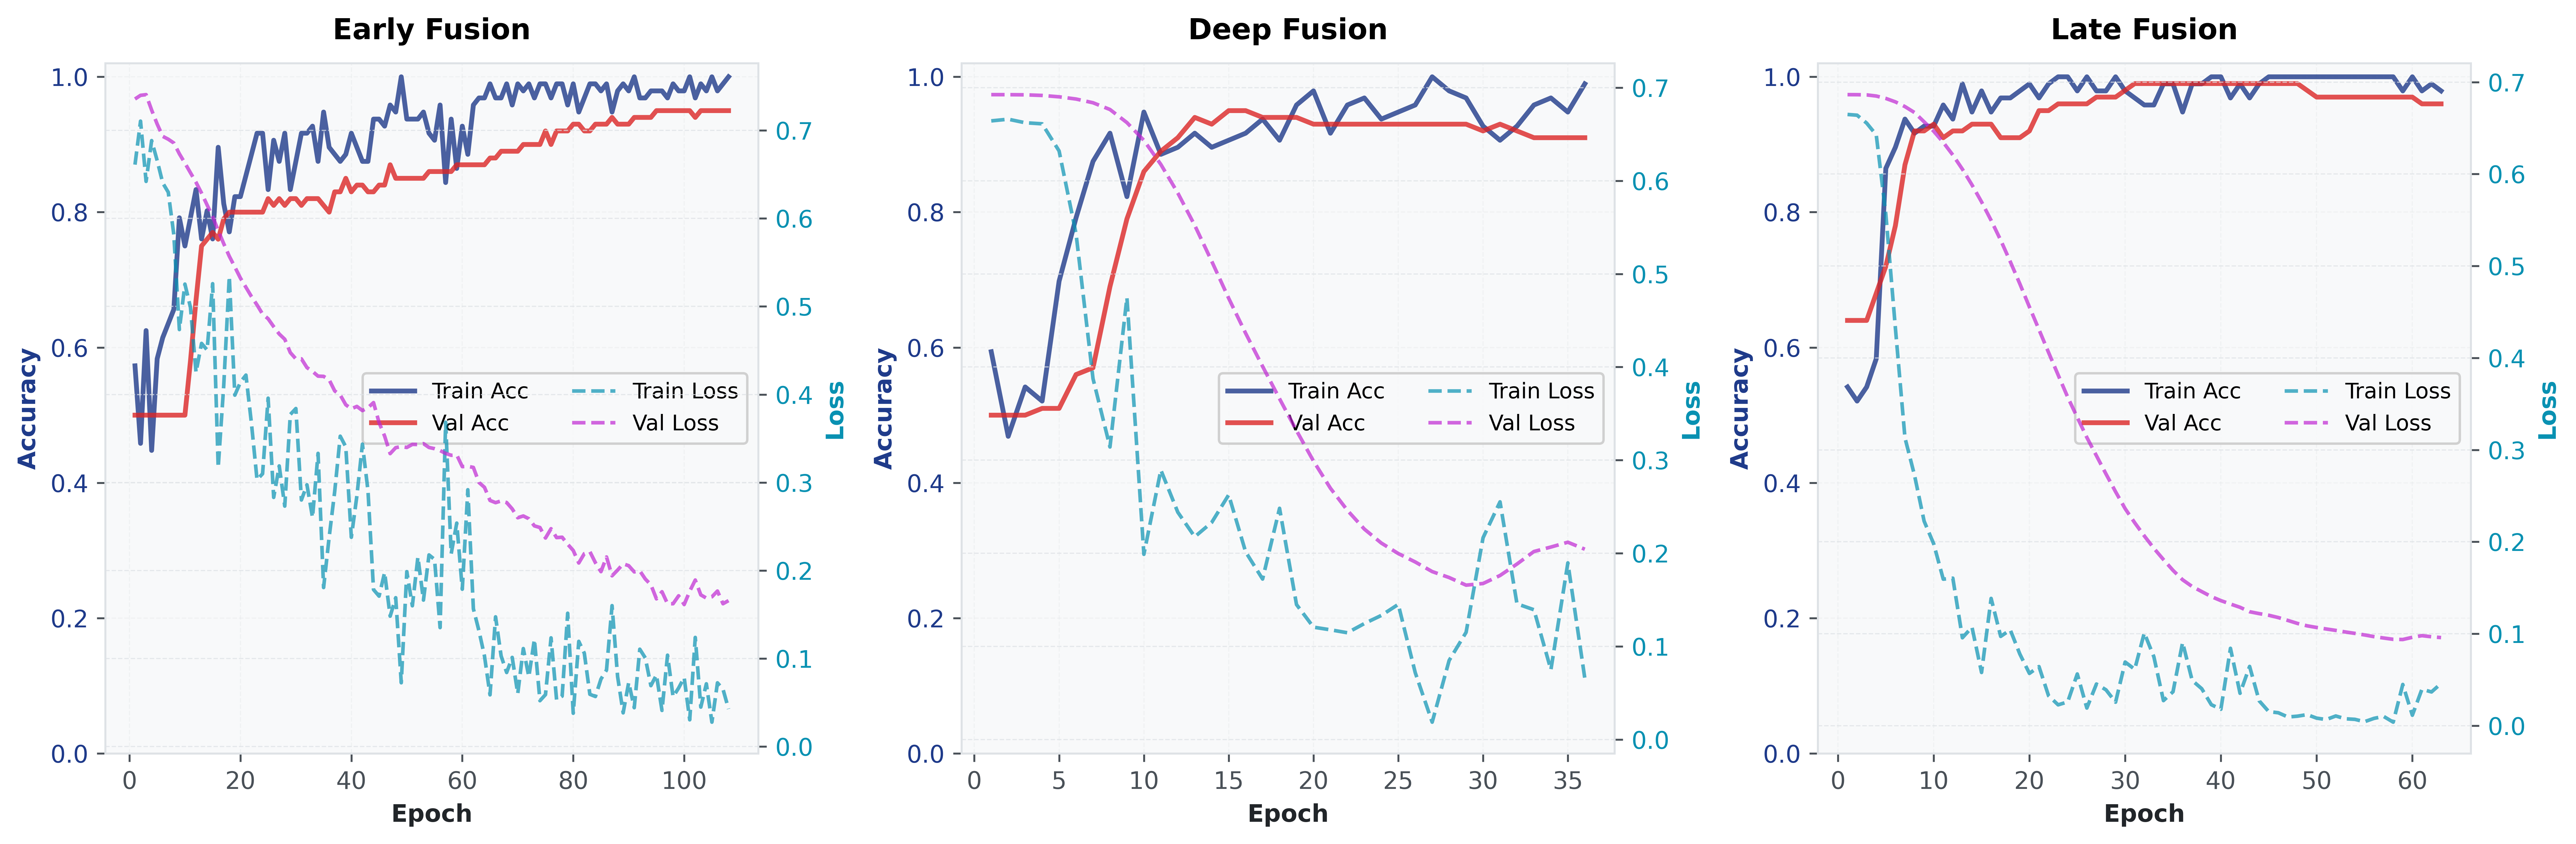
\includegraphics[width=1.0\textwidth]{images/accuracy-loss-curves.png}
    \caption{Training and validation accuracy and loss curves for the best models from each fusion strategy.}
    \label{accuracy-loss-curves}
\end{figure*}

Figure~\ref{auc-curves} illustrates the evolution of AUC during training, showing that all fusion strategies reached near-optimal discrimination performance within a limited number of epochs.

\begin{figure*}[!t]
    \centering
    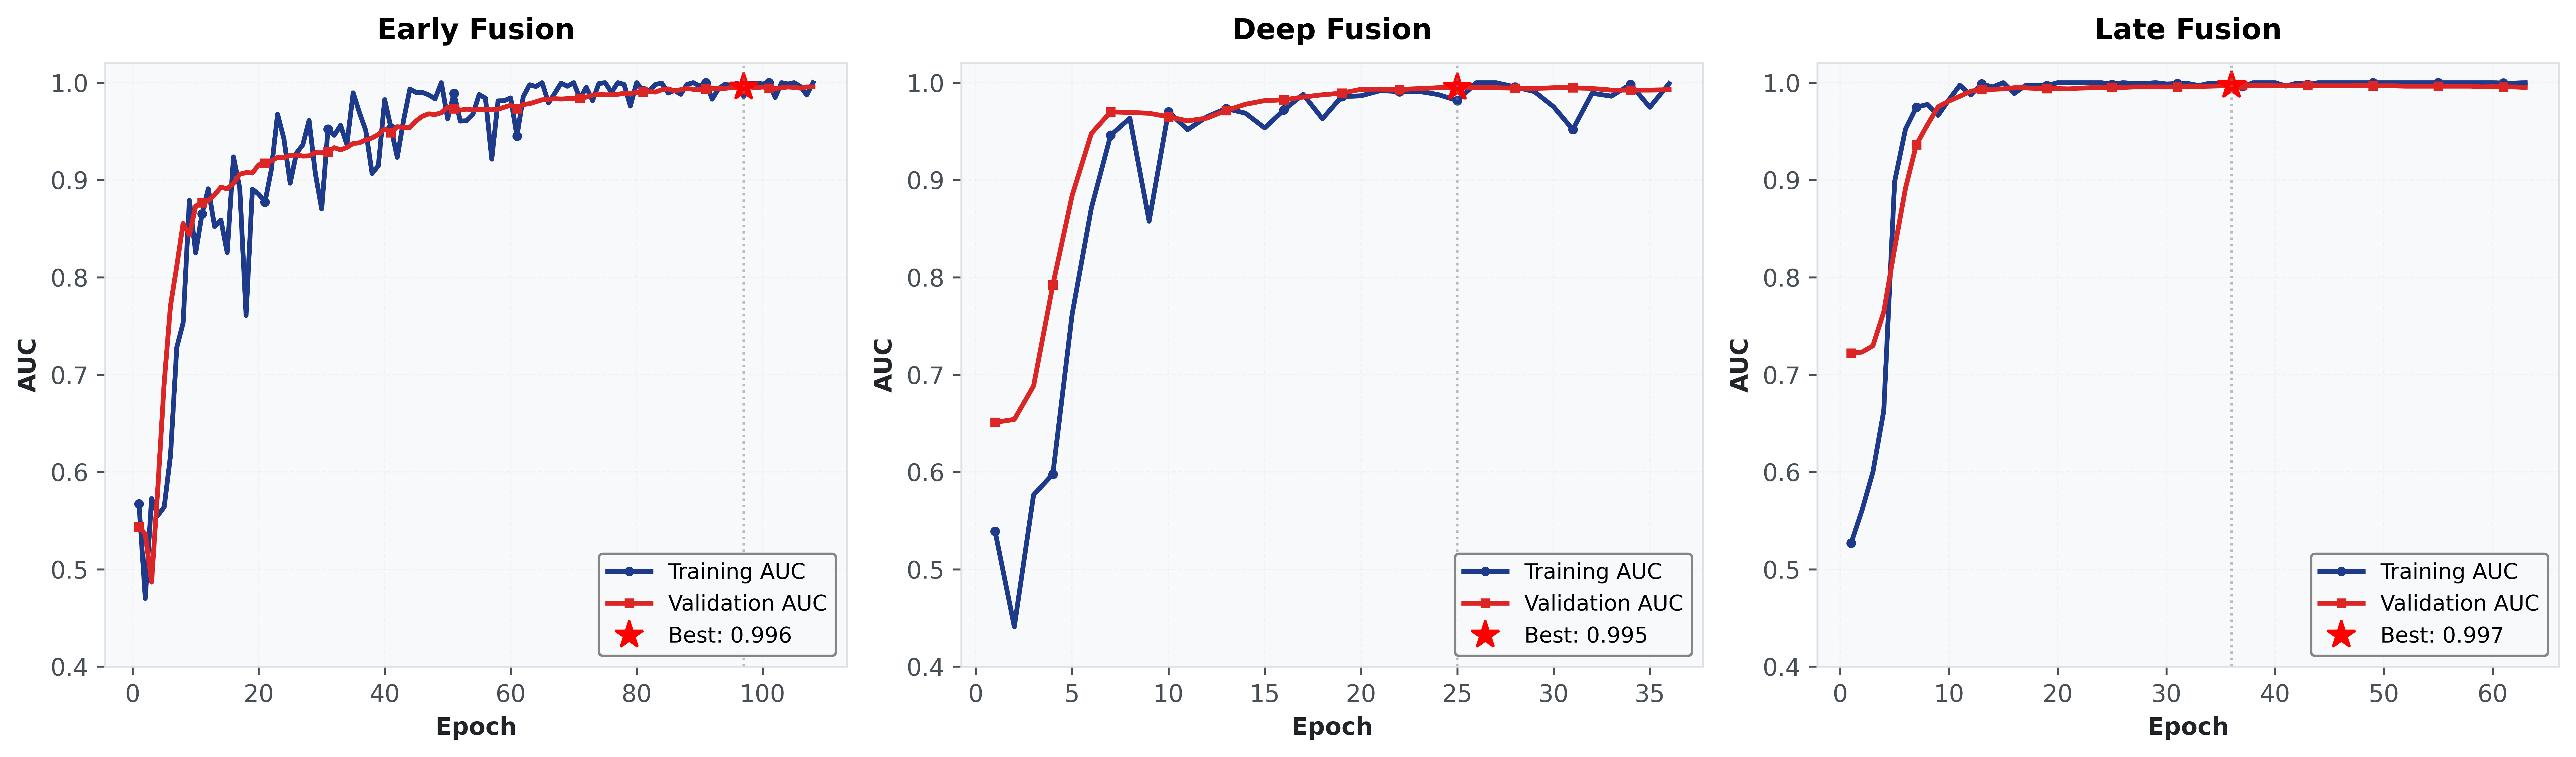
\includegraphics[width=1.0\textwidth]{images/auc-curves.png}
    \caption{AUC improvement over training epochs for each fusion strategy.}
    \label{auc-curves}
\end{figure*}


Receiver operating characteristic (ROC) and precision–recall (PR) curves for the test set are presented in Figure~\ref{roc-pr-curves}. Deep Fusion consistently dominates the ROC and PR spaces, reflecting superior trade-offs between sensitivity and specificity across operating points.

\begin{figure*}[!t]
    \centering
    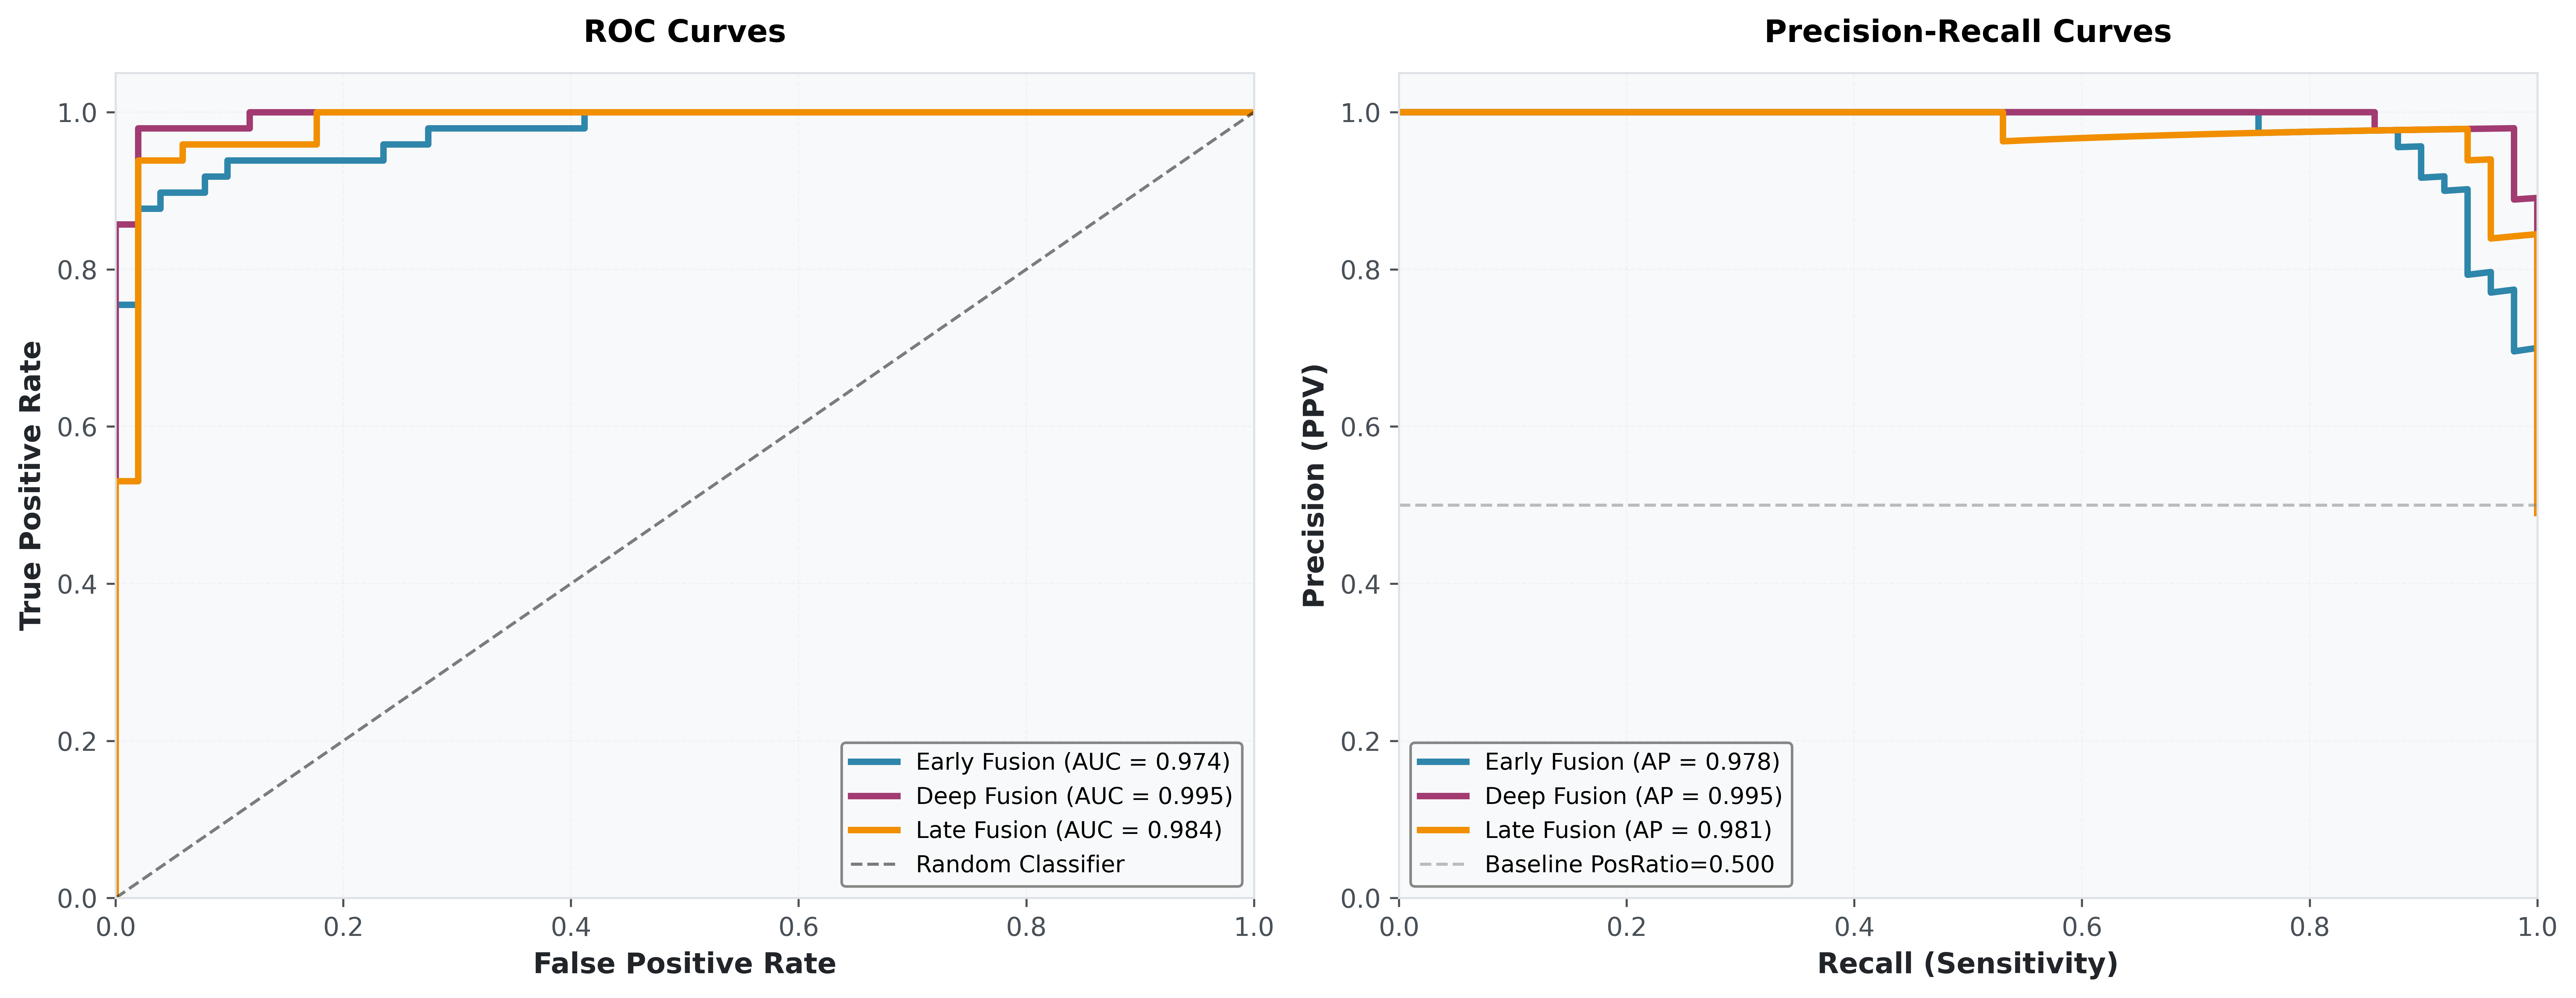
\includegraphics[width=0.9\textwidth]{images/roc-pr-curves.png}
    \caption{ROC and PR curves for the best models from each fusion strategy on the test set.}
    \label{roc-pr-curves}
\end{figure*}
Confusion matrices for the three fusion strategies are shown in Figure~\ref{confusion-matrices}. Deep Fusion achieved the lowest false-negative rate, misclassifying only one glaucomatous case, while correctly identifying 48 out of 49 positive samples. This reinforces its suitability for screening applications where recall is prioritized.

\begin{figure*}[!t]
    \centering
    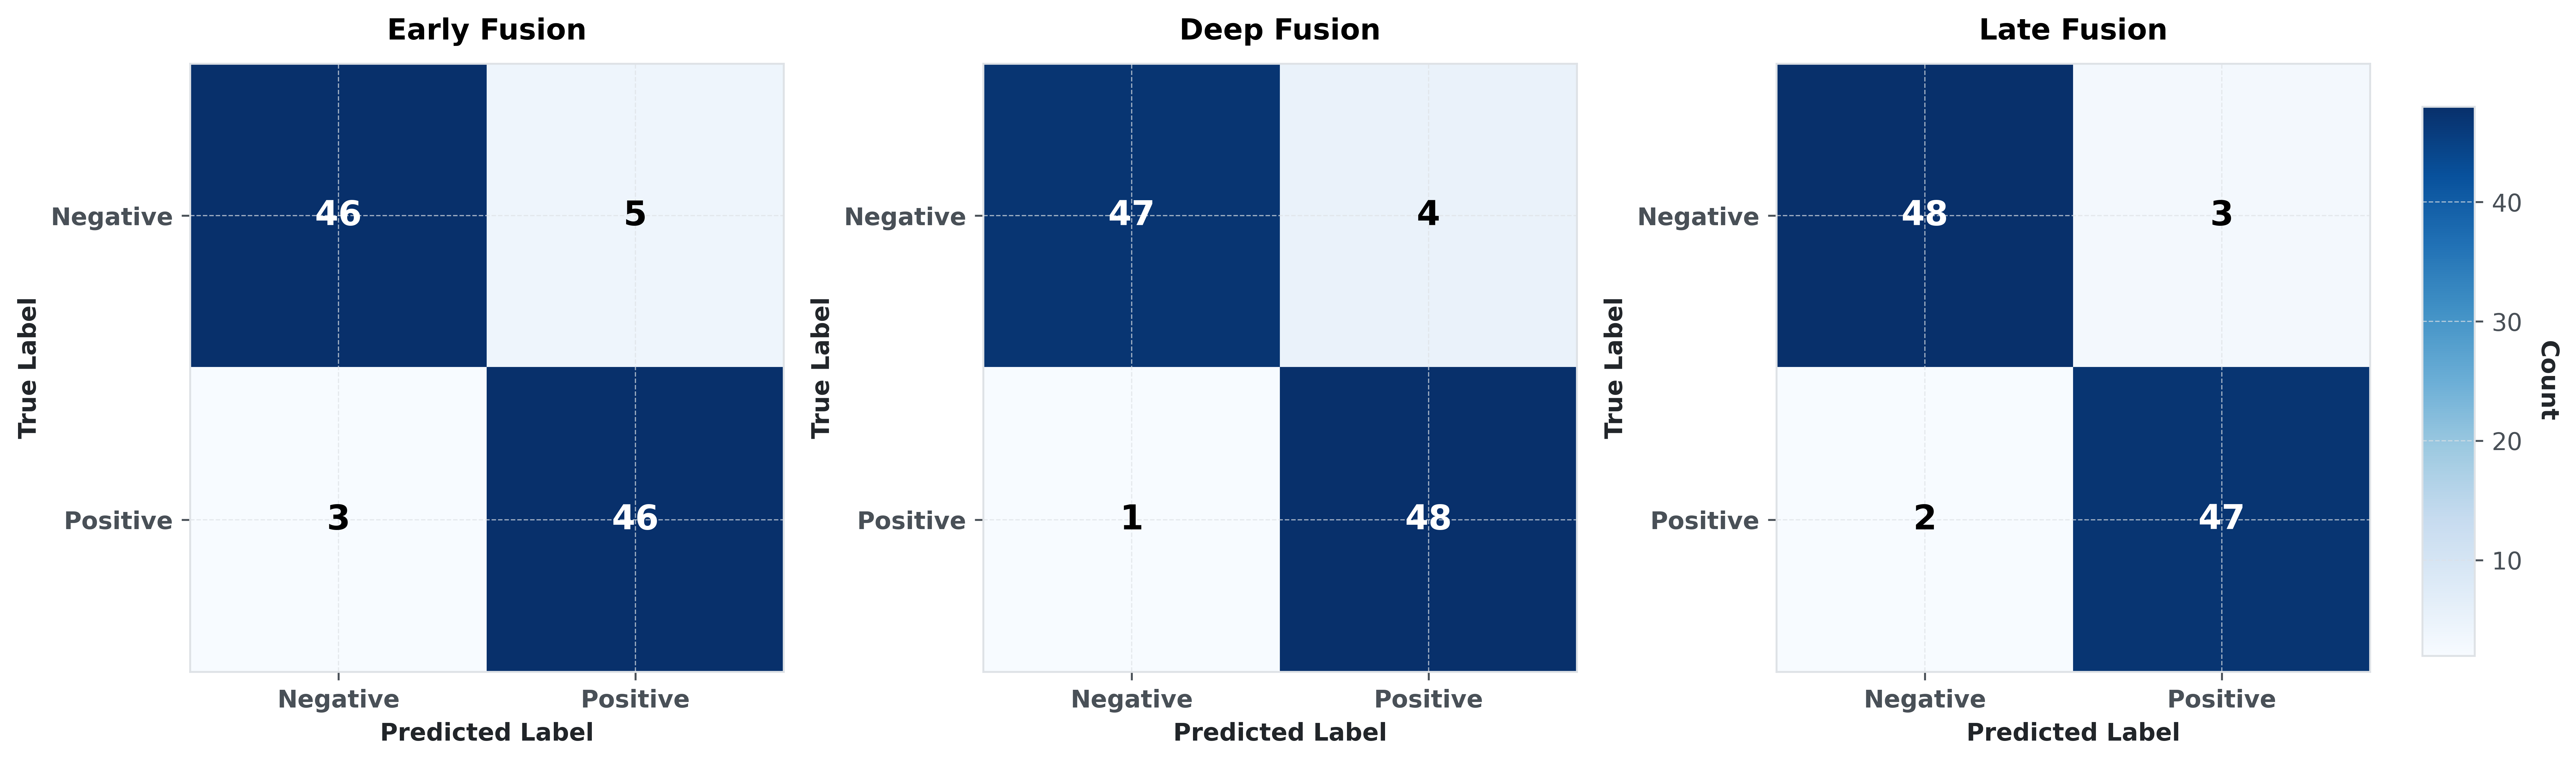
\includegraphics[width=0.9\textwidth]{images/confusion-matrices.png}
    \caption{Confusion matrices for the best models from each fusion strategy on the test set.}
    \label{confusion-matrices}
\end{figure*}
Model efficiency was also analyzed in terms of trainable parameters, floating-point operations (FLOPs), and inference latency (Figure~\ref{model-efficiency}). Deep Fusion achieved the most favorable balance between computational efficiency and predictive performance, exhibiting the lowest inference time while maintaining the highest accuracy.

\begin{figure*}[!t]
    \centering
    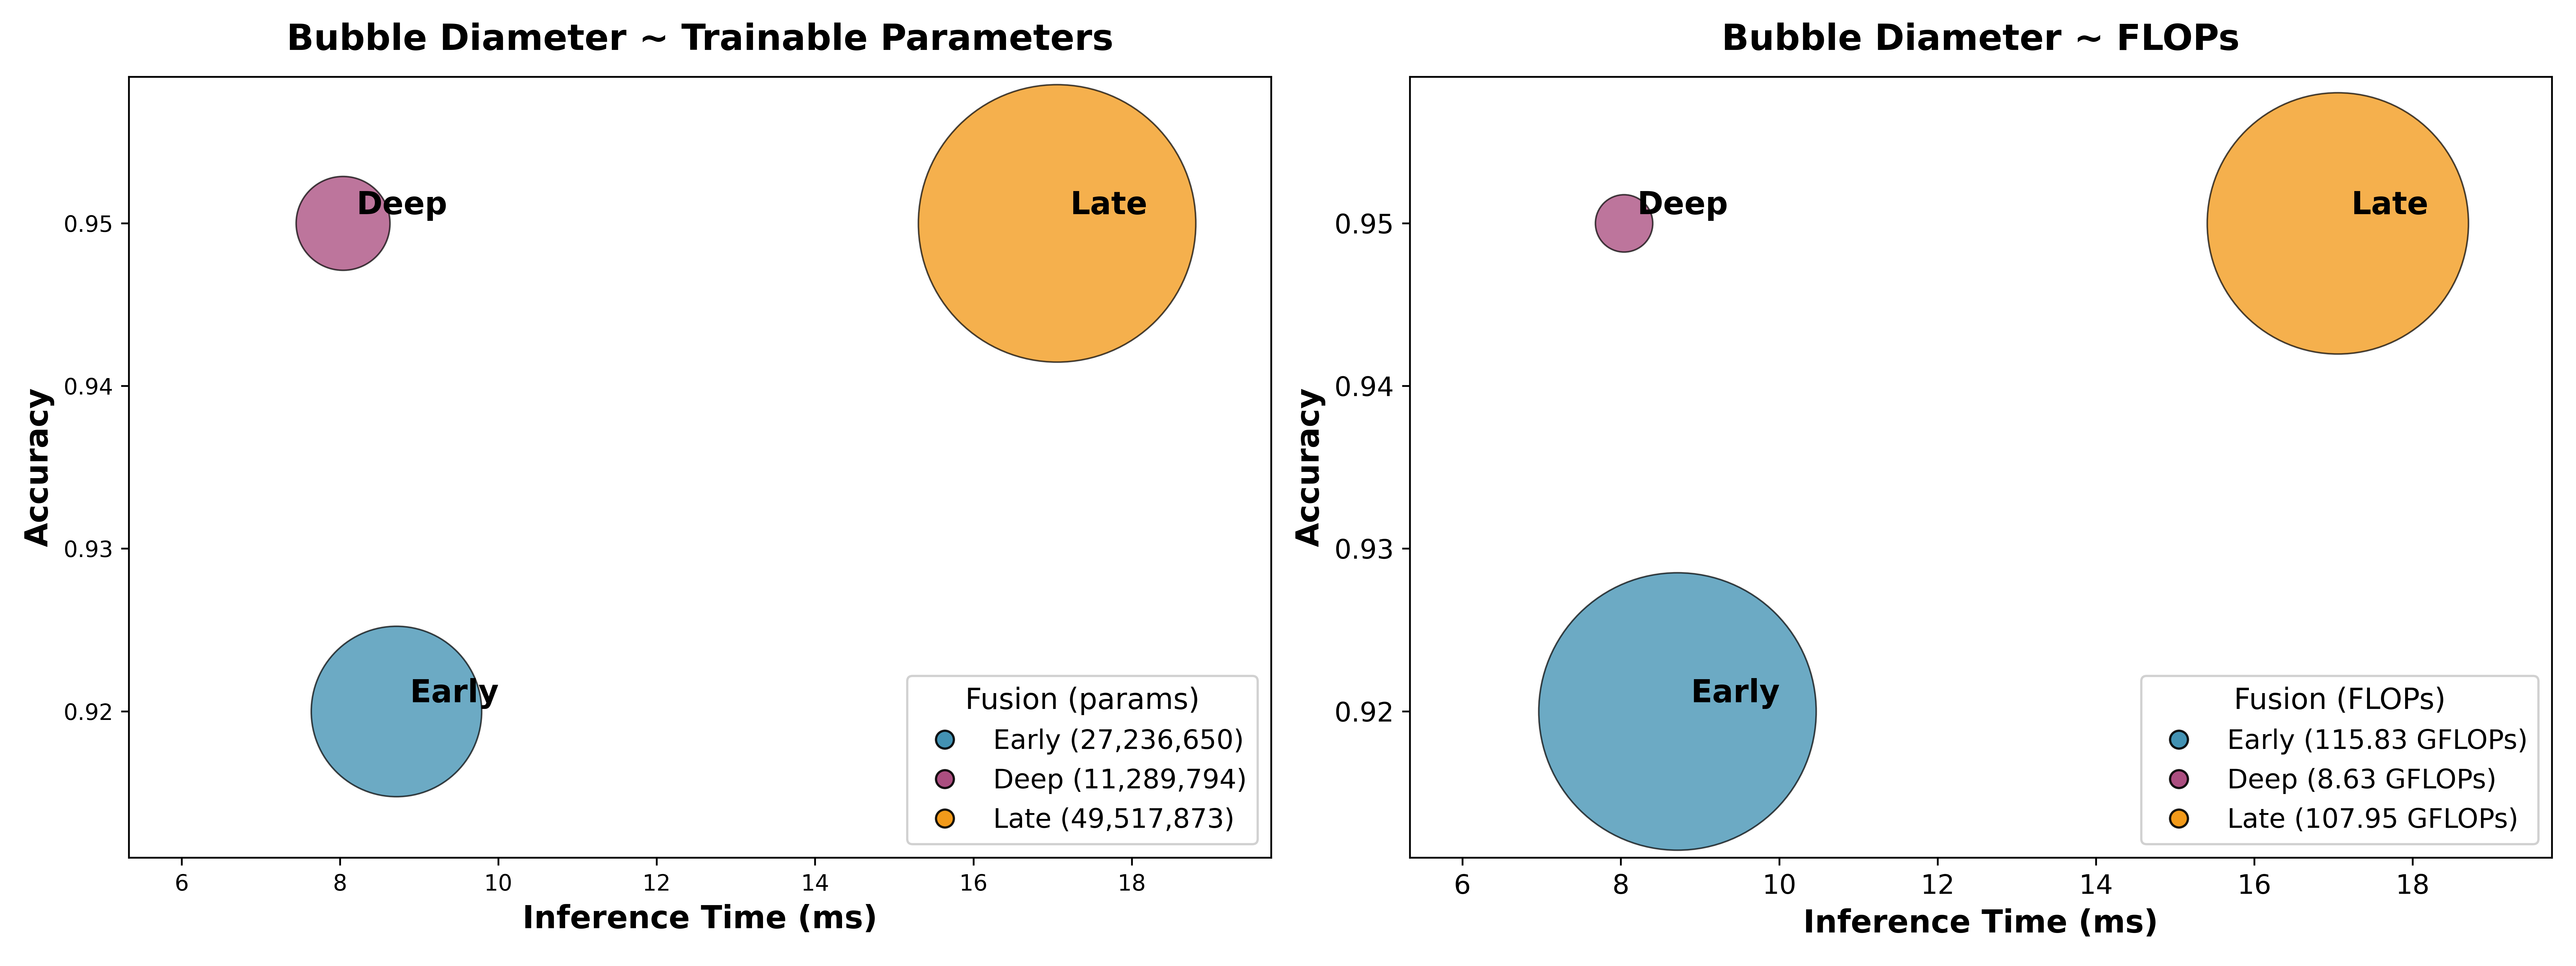
\includegraphics[width=1.0\textwidth]{images/model-efficiency.png}
    \caption{Model efficiency analysis: (left) Parameters vs Inference Time with bubble size representing number of parameters, (right) FLOPs vs Inference Time with bubble size representing FLOPs.}
    \label{model-efficiency}
\end{figure*}



\subsubsection{Five-Fold Cross-Validation Results}
\label{subsubsec:cv_binary}

To further assess robustness and generalization, five-fold stratified cross-validation was conducted for binary glaucoma screening after merging the original training and validation splits. Each fusion strategy was evaluated using identical folds and hyperparameter configurations identified during optimization.

Table~\ref{tab:cv_binary_compact} summarizes the five-fold cross-validation results using mean $\pm$ standard deviation, with minimum and maximum values across folds reported in brackets for completeness.

\begin{table*}[!t]
    \centering
    \caption{Five-fold cross-validation results for binary glaucoma screening (mean $\pm$ std [min, max]).}
    \label{tab:cv_binary_compact}
    \scriptsize
    \setlength{\tabcolsep}{6pt}
    \begin{tabular}{|l|c|c|c|}
        \hline
        \textbf{Metric}                & \textbf{Early Fusion} & \textbf{Deep Fusion} & \textbf{Late Fusion} \\
        \hline
        Accuracy                       &
        $0.894 \pm 0.023\,[0.87,0.93]$ &
        $0.924 \pm 0.027\,[0.89,0.96]$ &
        $0.934 \pm 0.016\,[0.91,0.96]$                                                                       \\

        AUC-ROC                        &
        $0.973 \pm 0.006\,[0.97,0.99]$ &
        $0.988 \pm 0.008\,[0.98,1.00]$ &
        $0.988 \pm 0.002\,[0.98,0.99]$                                                                       \\

        AUC-PR                         &
        $0.970 \pm 0.008\,[0.96,0.98]$ &
        $0.988 \pm 0.008\,[0.98,1.00]$ &
        $0.986 \pm 0.004\,[0.98,0.99]$                                                                       \\

        Precision (PPV)                &
        $0.937 \pm 0.015\,[0.92,0.96]$ &
        $0.916 \pm 0.017\,[0.88,0.93]$ &
        $0.951 \pm 0.027\,[0.90,0.98]$                                                                       \\

        Recall (Sens.)                 &
        $0.841 \pm 0.051\,[0.78,0.90]$ &
        $0.931 \pm 0.057\,[0.84,1.00]$ &
        $0.914 \pm 0.052\,[0.84,0.98]$                                                                       \\

        F1-score                       &
        $0.885 \pm 0.028\,[0.85,0.93]$ &
        $0.922 \pm 0.030\,[0.88,0.96]$ &
        $0.931 \pm 0.019\,[0.90,0.96]$                                                                       \\

        Cohen’s Kappa                  &
        $0.787 \pm 0.047\,[0.74,0.86]$ &
        $0.848 \pm 0.055\,[0.78,0.92]$ &
        $0.868 \pm 0.033\,[0.82,0.92]$                                                                       \\

        Brier Score                    &
        $0.082 \pm 0.010\,[0.07,0.09]$ &
        $0.054 \pm 0.027\,[0.02,0.09]$ &
        $0.054 \pm 0.016\,[0.04,0.08]$                                                                       \\
        \hline
    \end{tabular}
\end{table*}


All fusion strategies demonstrated stable and consistently high performance across folds, confirming the robustness of the proposed framework. Deep Fusion achieved the highest mean recall, reinforcing its suitability for screening scenarios where minimizing false negatives is critical. Late Fusion achieved the highest mean accuracy and Cohen’s kappa, indicating strong agreement and stable decision behavior.

Figure~\ref{cv-metric-boxplots} illustrates the distribution of major performance metrics across folds, highlighting reduced variance for Deep and Late Fusion strategies.

\begin{figure*}[!t]
    \centering
    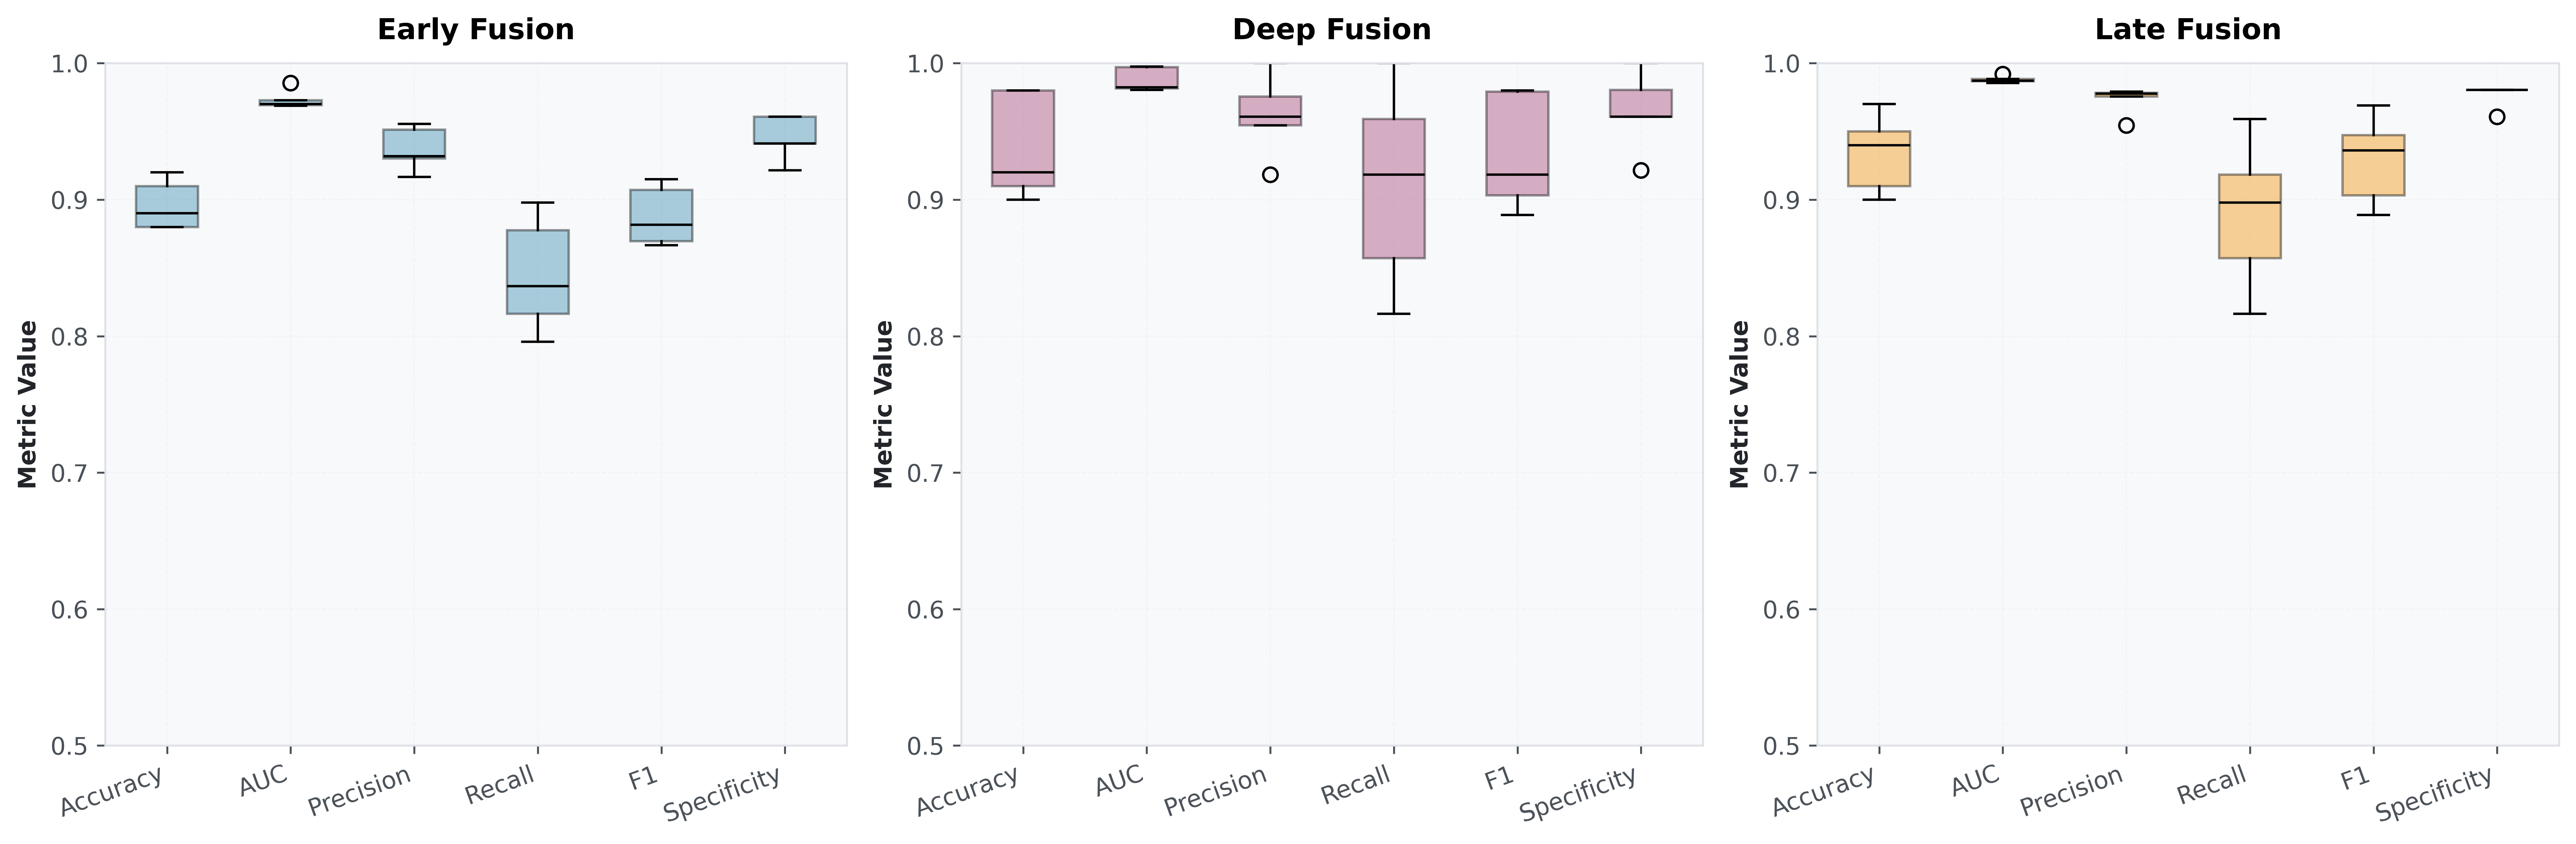
\includegraphics[width=1.0\textwidth]{images/cv-metric-boxplots.png}
    \caption{Five-fold cross-validation: box plots of accuracy, AUC-ROC, precision, recall, F1-score and specificity metrics for each fusion strategy.}
    \label{cv-metric-boxplots}
\end{figure*}

Averaged training and validation curves (Figure~\ref{cv-accuracy-loss-curves}) confirm stable convergence without overfitting across all folds. Consistent with single-fold results, Deep Fusion converges faster than the other strategies across data splits, while Late Fusion exhibits fewer fluctuations in accuracy and loss, indicating greater training stability more likely due to independent feature learning before fusion and reduced augmentation impact.

\begin{figure*}[!t]
    \centering
    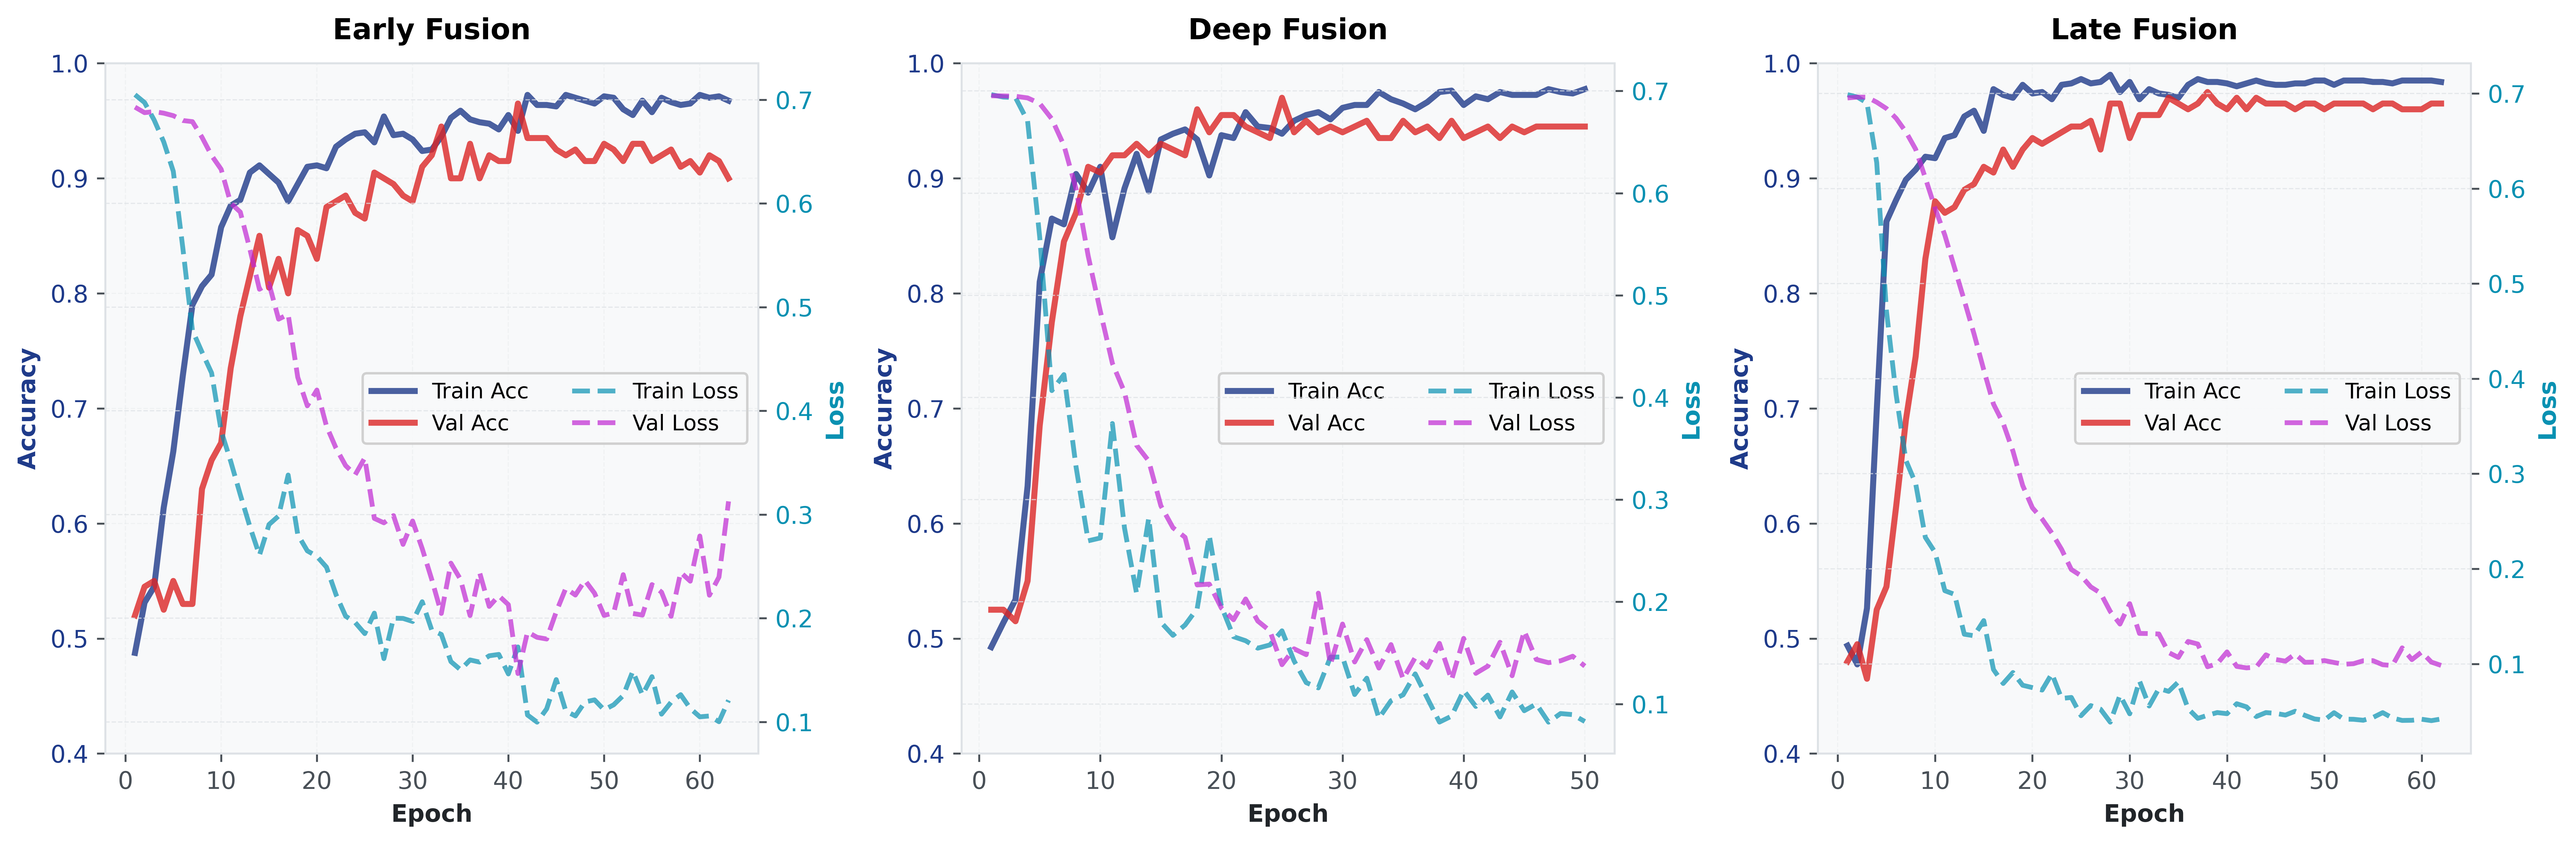
\includegraphics[width=1.0\textwidth]{images/cv-accuracy-loss-curves.png}
    \caption{Five-fold cross-validation: averaged training and validation accuracy and loss curves for the best models from each fusion strategy.}
    \label{cv-accuracy-loss-curves}
\end{figure*}

Figure~\ref{cv-auc-curves} shows the averaged AUC progression over epochs for each strategy across five-folds, with shaded regions representing variability. All strategies reached optimal performance early, prior to early stopping activation.

\begin{figure*}[!t]
    \centering
    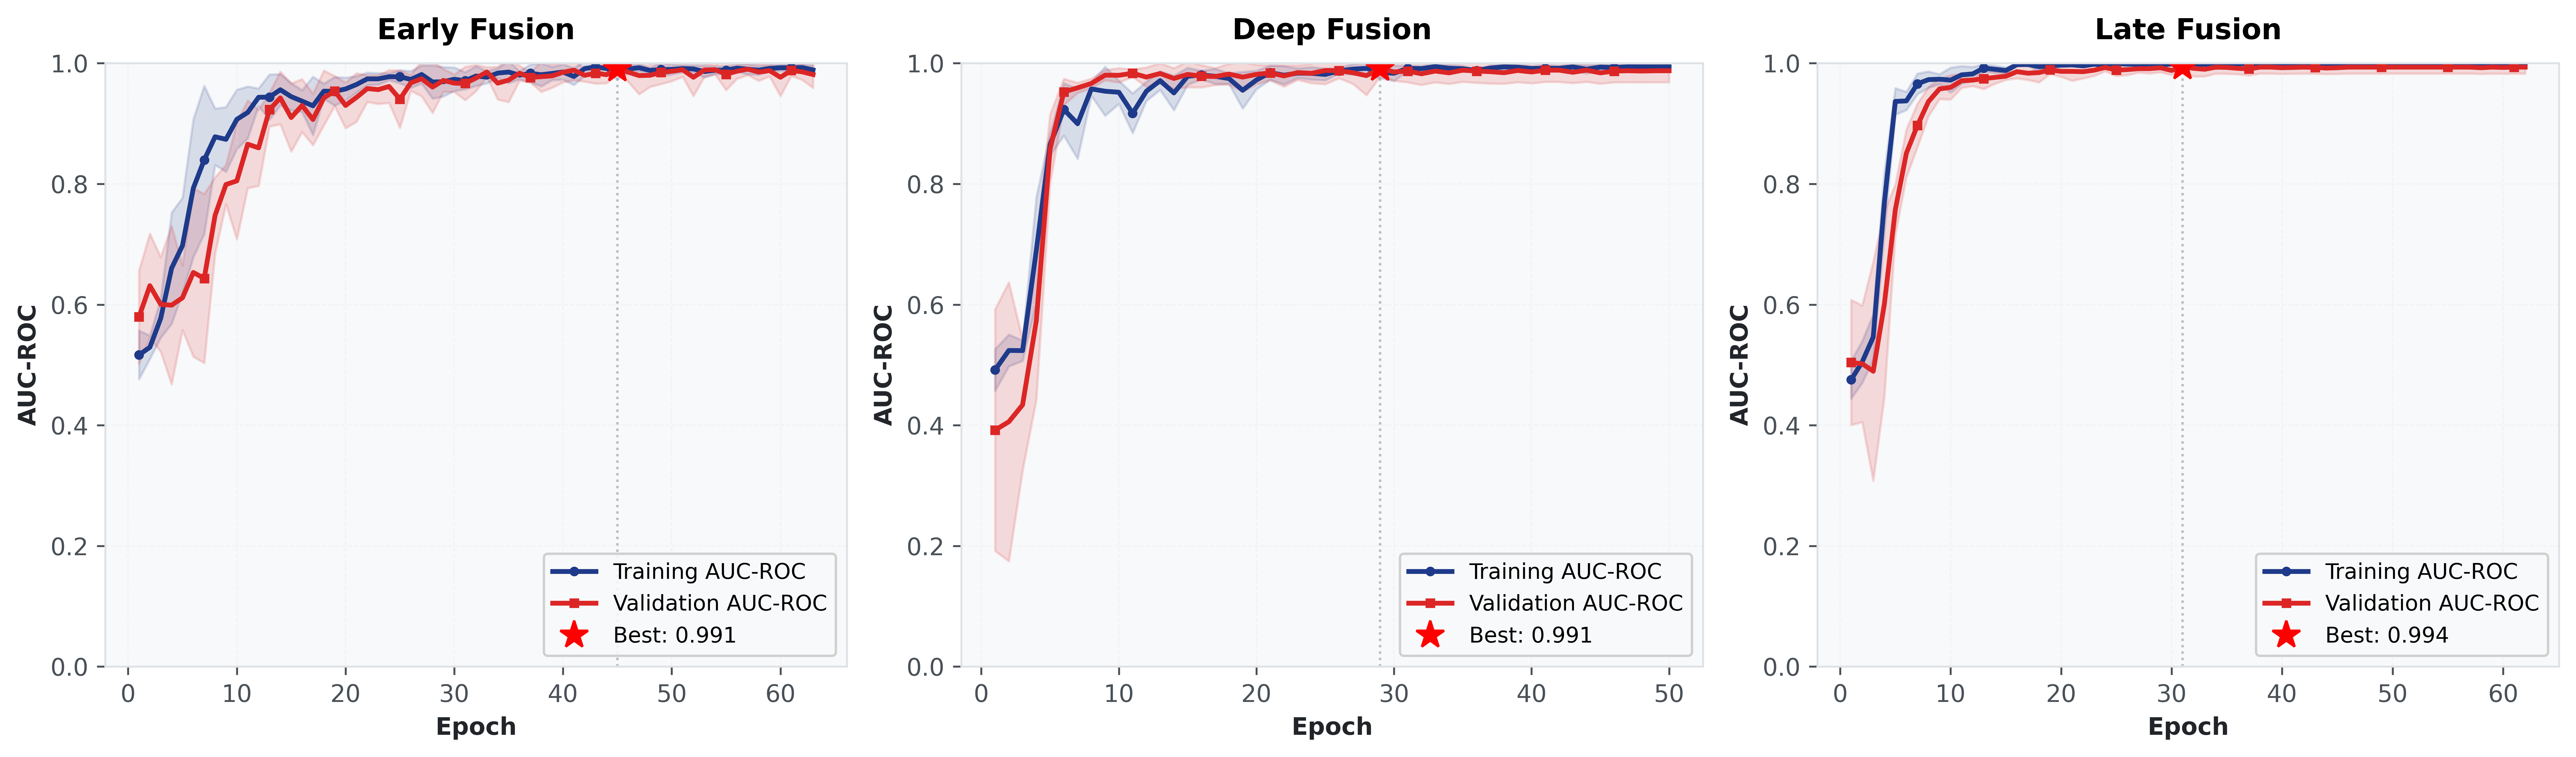
\includegraphics[width=1.0\textwidth]{images/cv-auc-curves.png}
    \caption{Five-fold cross-validation: averaged AUC improvement over training epochs for each fusion strategy. Shaded regions represent range of AUC values across folds at each epoch.}
    \label{cv-auc-curves}
\end{figure*}
Consistent with single-split results, Deep Fusion converged more rapidly, while Late Fusion exhibited smoother optimization dynamics. Averaged ROC and PR curves across folds (Figure~\ref{cv-roc-pr-curves}) further confirm strong discrimination capability, with Late Fusion slightly dominating the upper envelope.

\begin{figure*}[!t]
    \centering
    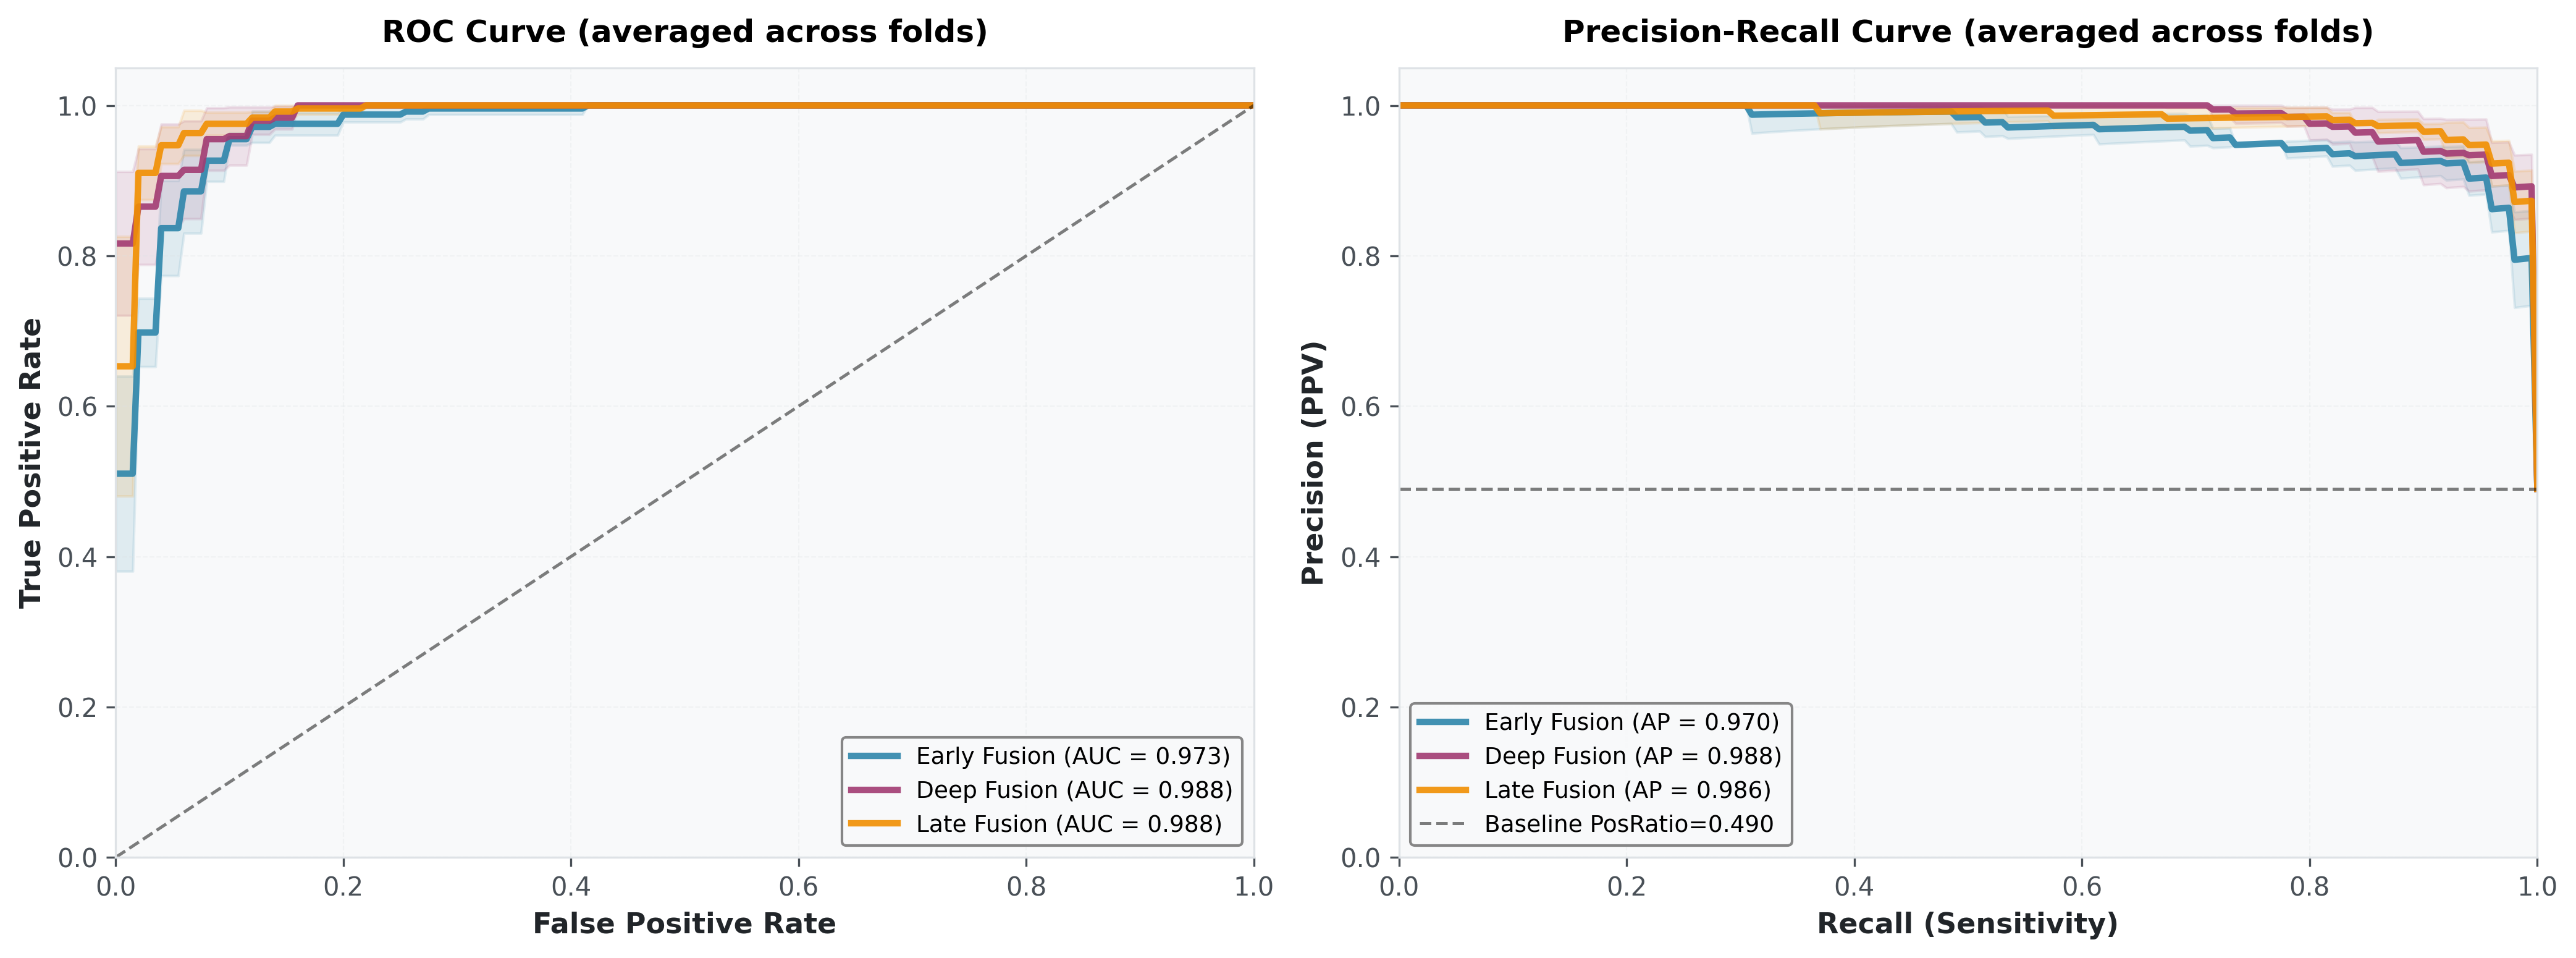
\includegraphics[width=0.9\textwidth]{images/cv-roc-pr-curves.png}
    \caption{Five-fold cross-validation: averaged ROC and PR curves across folds for the best models from each fusion strategy on the test sets.}
    \label{cv-roc-pr-curves}
\end{figure*}
Accumulated confusion matrices across folds (Figure~\ref{cv-confusion-matrices}) show that Deep Fusion consistently achieved the lowest false-negative rate, while both Deep and Late Fusion maintained high true-positive and true-negative counts compared to Early Fusion.

\begin{figure*}[!t]
    \centering
    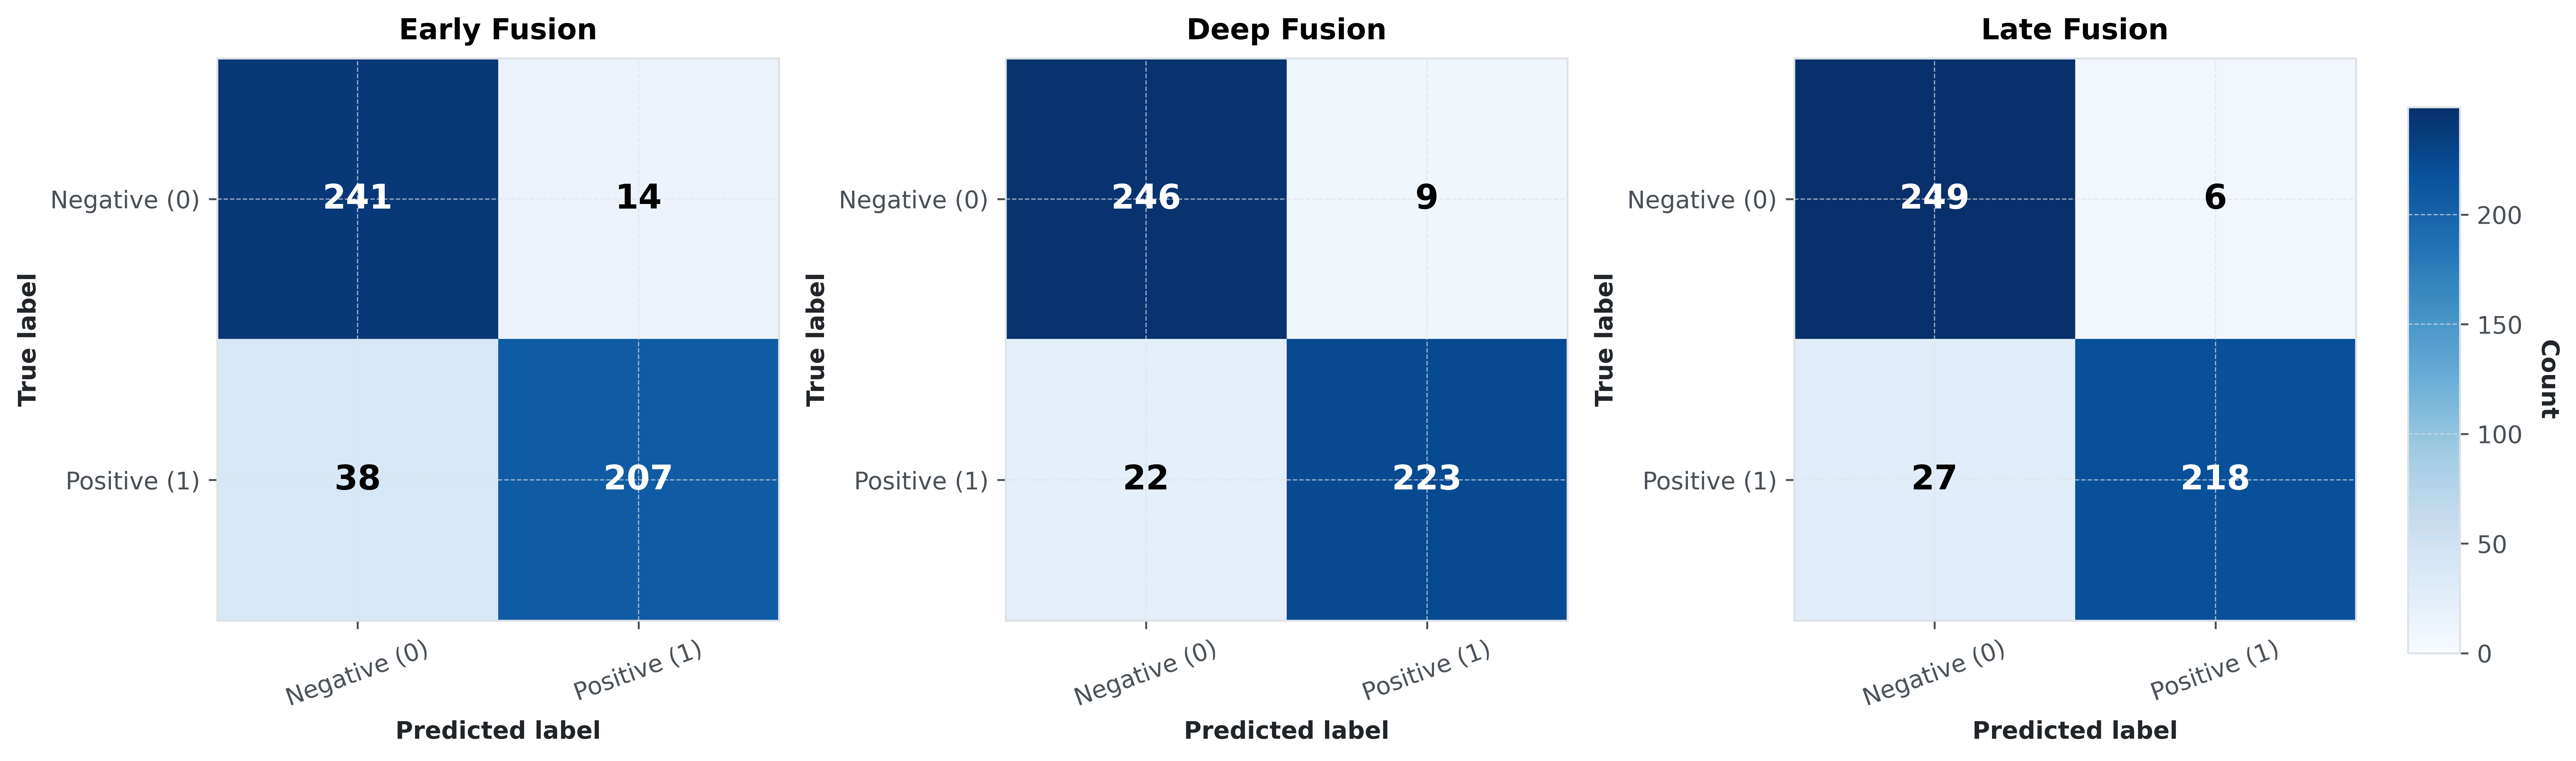
\includegraphics[width=0.9\textwidth]{images/cv-confusion-matrices.png}
    \caption{Five-fold cross-validation: confusion matrices with accumulated counts across folds for the best models from each fusion strategy on the test sets.}
    \label{cv-confusion-matrices}
\end{figure*}

Having established robustness for screening, we next evaluate grading performance under class imbalance and uncertainty-aware reporting.

\subsection{MULTICLASS GLAUCOMA GRADING RESULTS}
\label{subsec:multiclass_results}

This subsection evaluates the proposed multimodal fusion framework under the multiclass glaucoma grading protocol, where each eye is categorized into non-glaucoma, early glaucoma, or mid--advanced glaucoma. Unlike binary screening, glaucoma grading introduces ordinal structure, class imbalance, and increased decision uncertainty, making robust evaluation essential. We therefore report both point-estimate performance on a held-out test split and uncertainty-aware results using bootstrap-based confidence interval estimation.

\subsubsection{Default Single Split Test Results}
\label{subsubsec:multiclass_single_split}

Table~\ref{tab:multiclass_single_split_metrics} summarizes the multiclass grading performance obtained on the held-out test set for Early, Deep, and Late Fusion strategies. Performance is reported using accuracy, Cohen’s kappa, quadratically weighted kappa (QWK), macro- and weighted-F1 scores, macro-averaged precision and recall, and one-vs-rest (OvR) AUC-ROC. These metrics jointly capture overall correctness, inter-class agreement, ordinal consistency, and class-balanced discrimination.

\begin{table}[!t]
    \centering
    \caption{Multiclass glaucoma grading performance on the held-out test set (default split).}
    \label{tab:multiclass_single_split_metrics}
    \scriptsize
    \setlength{\tabcolsep}{6pt}
    \resizebox{\columnwidth}{!}{%
        \begin{tabular}{|l|c|c|c|}
            \hline
            \textbf{Metric} & \textbf{Early Fusion} & \textbf{Deep Fusion} & \textbf{Late Fusion} \\
            \hline
            Accuracy
                            & 0.7400
                            & \textbf{0.8100}
                            & 0.7800                                                              \\
            \hline
            F1-score (Macro)
                            & 0.6770
                            & \textbf{0.7557}
                            & 0.7424                                                              \\
            \hline
            F1-score (Weighted)
                            & 0.7386
                            & \textbf{0.8070}
                            & 0.7907                                                              \\
            \hline
            Precision (Macro)
                            & 0.6787
                            & \textbf{0.7570}
                            & 0.7428                                                              \\
            \hline
            Recall (Macro)
                            & 0.6755
                            & \textbf{0.7569}
                            & 0.7504                                                              \\
            \hline
            AUC-ROC (OvR)
                            & 0.8783
                            & 0.9129
                            & \textbf{0.9165}                                                     \\
            \hline
            Cohen’s Kappa
                            & 0.5787
                            & \textbf{0.6923}
                            & 0.6552                                                              \\
            \hline
            Quadratically Weighted Kappa
                            & 0.8065
                            & \textbf{0.8633}
                            & 0.8355                                                              \\
            \hline
        \end{tabular}}
\end{table}


Across fusion strategies, all models achieved competitive multiclass grading performance, with Deep Fusion obtaining the highest QWK, indicating stronger alignment with the ordinal structure of glaucoma severity. Early and Late Fusion also showed strong class-balanced performance, demonstrating that the proposed framework generalizes well from binary screening to multiclass grading with minimal task-specific modification.

The grading results further emphasize the importance of effective multimodal interaction. Glaucoma progression often manifests through subtle structural variations across multiple retinal regions and layers. Deep Fusion integrates modality representations at an intermediate latent stage, enabling richer interaction between global fundus context and localized OCT-derived structural information while preserving modality-specific features. In contrast, Early Fusion may dilute modality-specific cues when modalities are combined at the pixel level, whereas Late Fusion limits interaction to the prediction stage. In addition, the OCT-MIL aggregation mechanism highlights diagnostically informative B-scan slices within OCT volumes, improving volumetric representation quality. Together, these factors contribute to the stronger ordinal agreement and grading performance observed for Deep Fusion.

Training and validation accuracy and loss trajectories for the three fusion strategies are illustrated in Figure~\ref{fig:multiclass_acc_loss_curves}. During the initial training epochs, all models exhibited a brief entropy collapse phenomenon, where predictions were biased toward the majority class before meaningful class-discriminative patterns were learned. This behavior is reflected by near-constant validation accuracy around random-chance levels (approximately 0.5), despite a monotonic decrease in training loss. As training progressed, the models gradually recovered from this regime and began learning balanced class representations, leading to steady improvements in validation performance.

The vertical dashed line indicates the epoch corresponding to the best validation checkpoint selected for inference, confirming that optimal models were captured prior to any overfitting. Compared to Deep and Late Fusion strategies, Early Fusion shows higher loss fluctuations throughout training, highlighting the increased difficulty of multiclass learning under aggressive augmentation and limited sample availability when fusion occurs at the pixel level.


\begin{figure*}[!t]
    \centering
    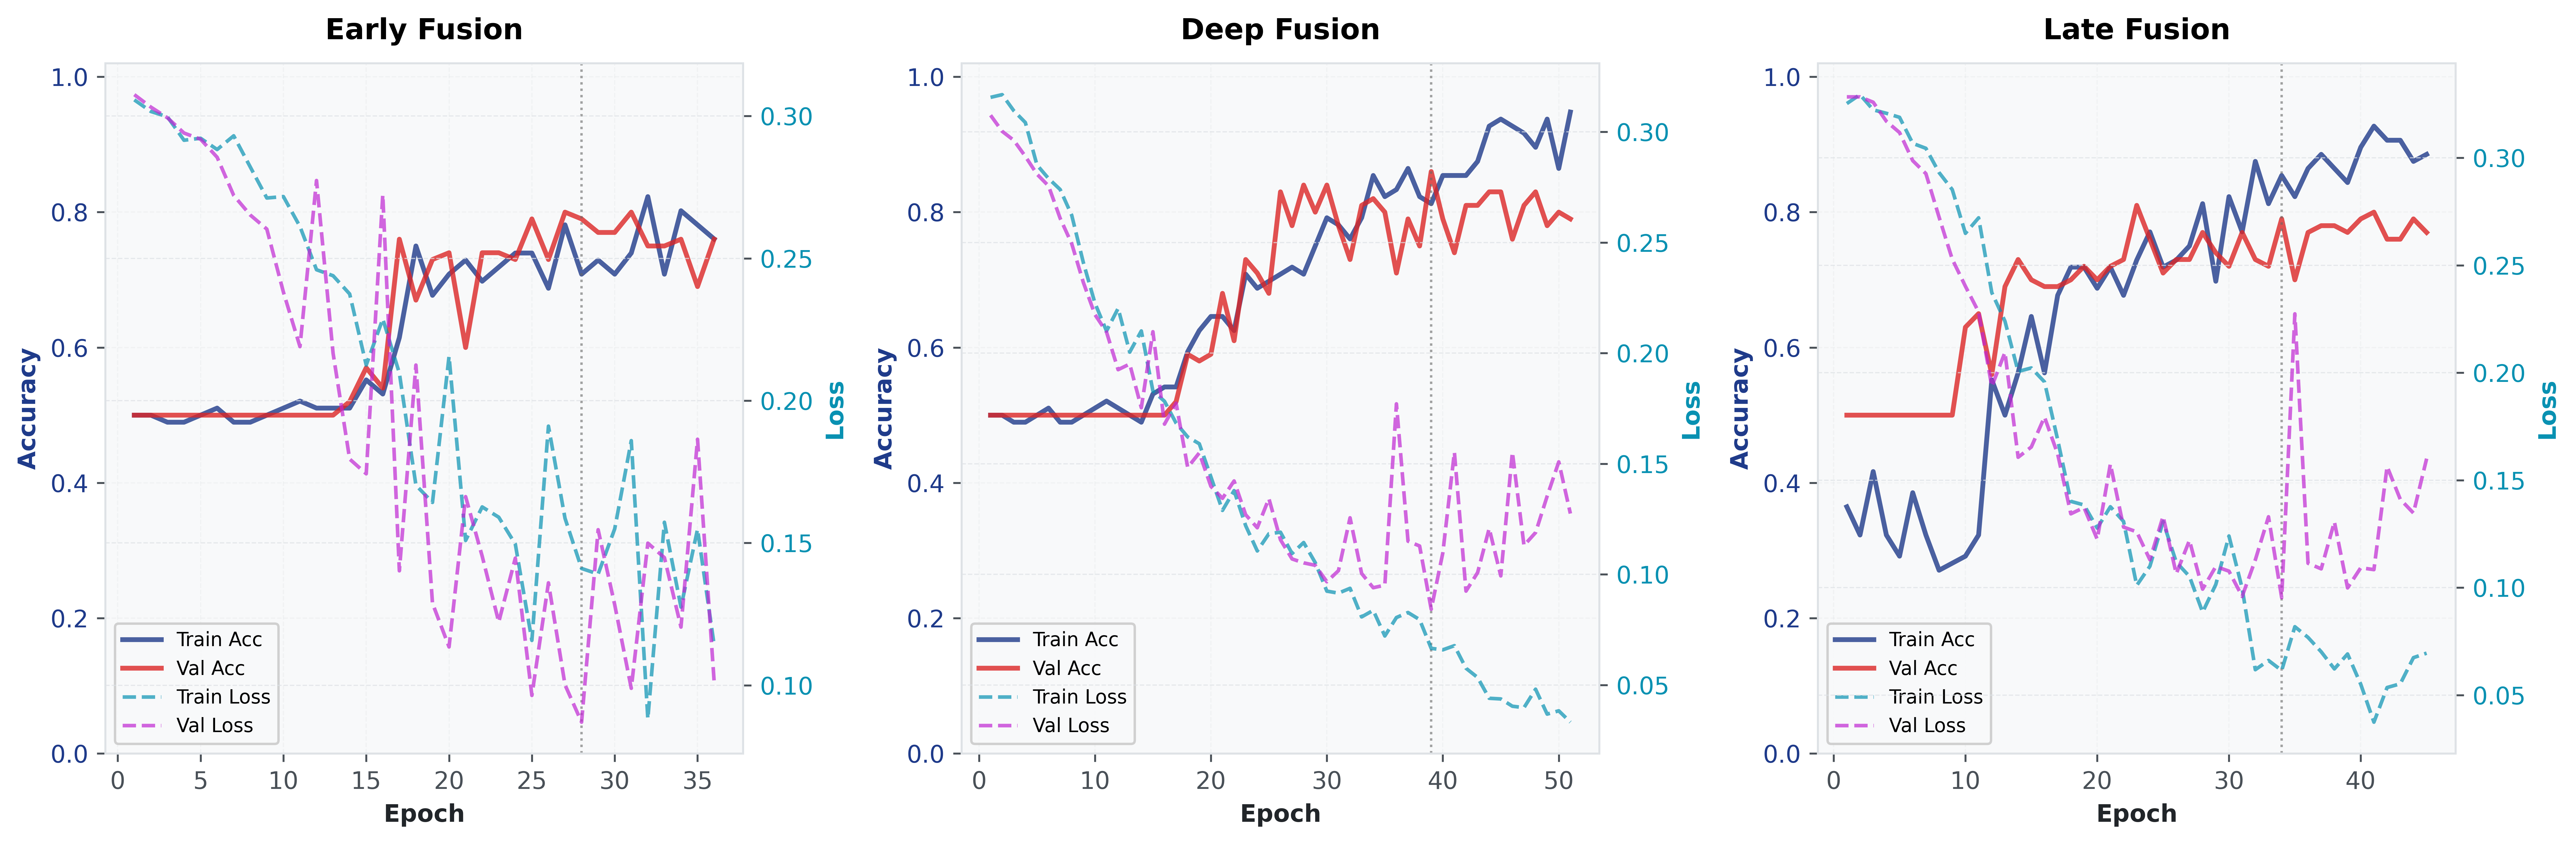
\includegraphics[width=1.0\textwidth]{images/multiclass_acc_loss_curves.png}
    \caption{Training and validation accuracy and loss curves for the best models from each fusion strategy under multiclass glaucoma grading.}
    \label{fig:multiclass_acc_loss_curves}
\end{figure*}

To better characterize optimization behavior under ordinal supervision, Figure~\ref{fig:multiclass_val_f1_qwk_curves} presents epoch-wise validation macro-F1 and QWK trends. In the early training phase, both metrics remain largely stationary at their initial values, reflecting the same entropy collapse observed in accuracy curves, where predictions are dominated by the majority class. Once this regime is resolved, macro-F1 and QWK begin to improve progressively across all fusion strategies. Despite fluctuations, the overall trajectories demonstrate an upward trend, eventually the trend stabilizing near their respective maxima in later epochs, indicating reliable convergence for multiclass glaucoma grading.


\begin{figure*}[!t]
    \centering
    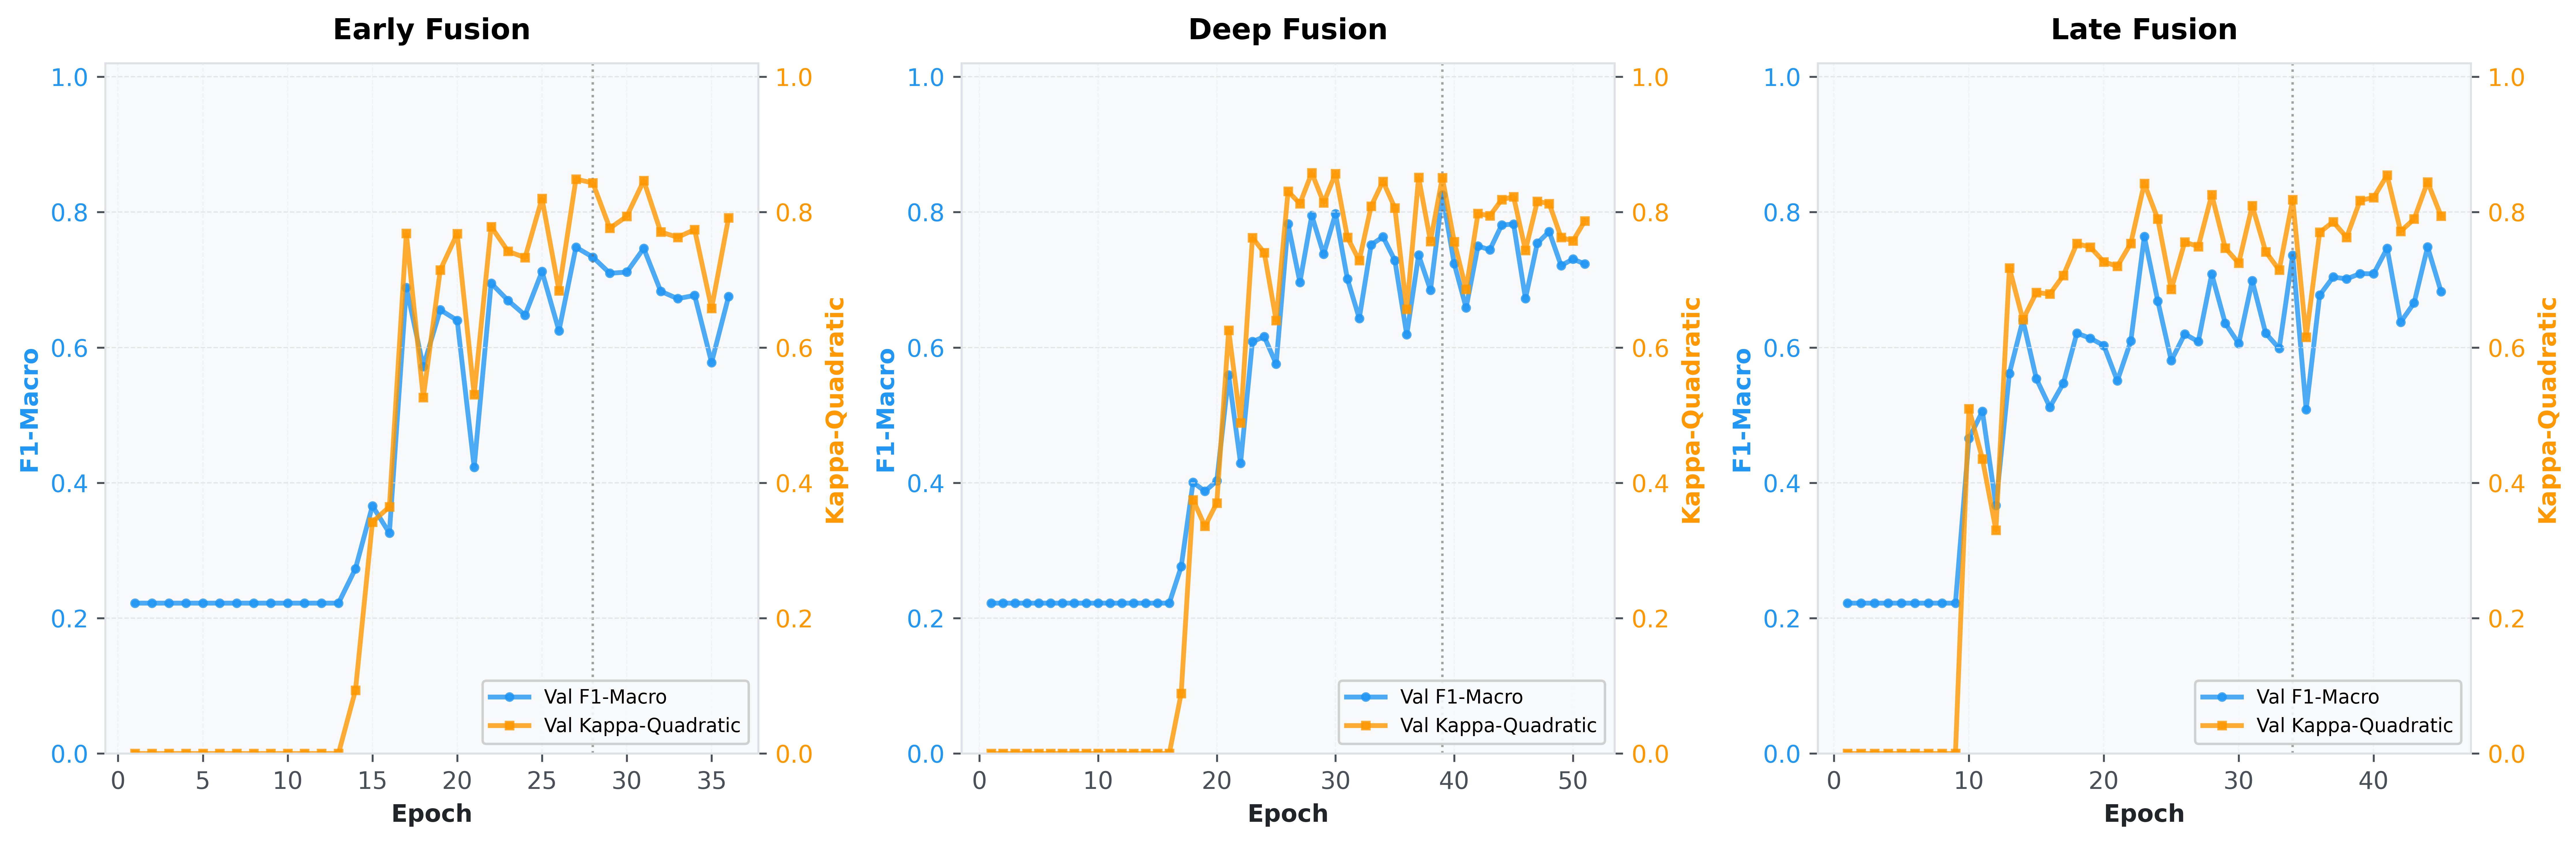
\includegraphics[width=1.0\textwidth]{images/multiclass_val_f1_qwk_curves.png}
    \caption{Validation macro-F1 and QWK improvement over training epochs for each fusion strategy under multiclass glaucoma grading.}
    \label{fig:multiclass_val_f1_qwk_curves}
\end{figure*}

Class-wise precision, recall, and F1-scores for each fusion strategy are illustrated in Figure~\ref{fig:multiclass_classwise_metrics}. Across all models, the majority class (non-glaucoma) achieves the highest scores, followed by the severe glaucoma class, while performance is comparatively weaker for the intermediate (early glaucoma) class. This behavior is expected in ordinal grading, where early-stage cases exhibit greater visual ambiguity and overlapping characteristics with adjacent classes. Among the fusion strategies, Deep Fusion attains the highest overall class-wise F1-scores, indicating superior representation alignment across severity levels. Late Fusion, however, shows comparatively stronger precision for the normal class and higher recall for the early class, which may be attributed to its decision-level confidence calibration that favors conservative predictions near class boundaries. Collectively, these trends confirm effective severity discrimination without collapse in minority or transitional classes.

\begin{figure*}[!t]
    \centering
    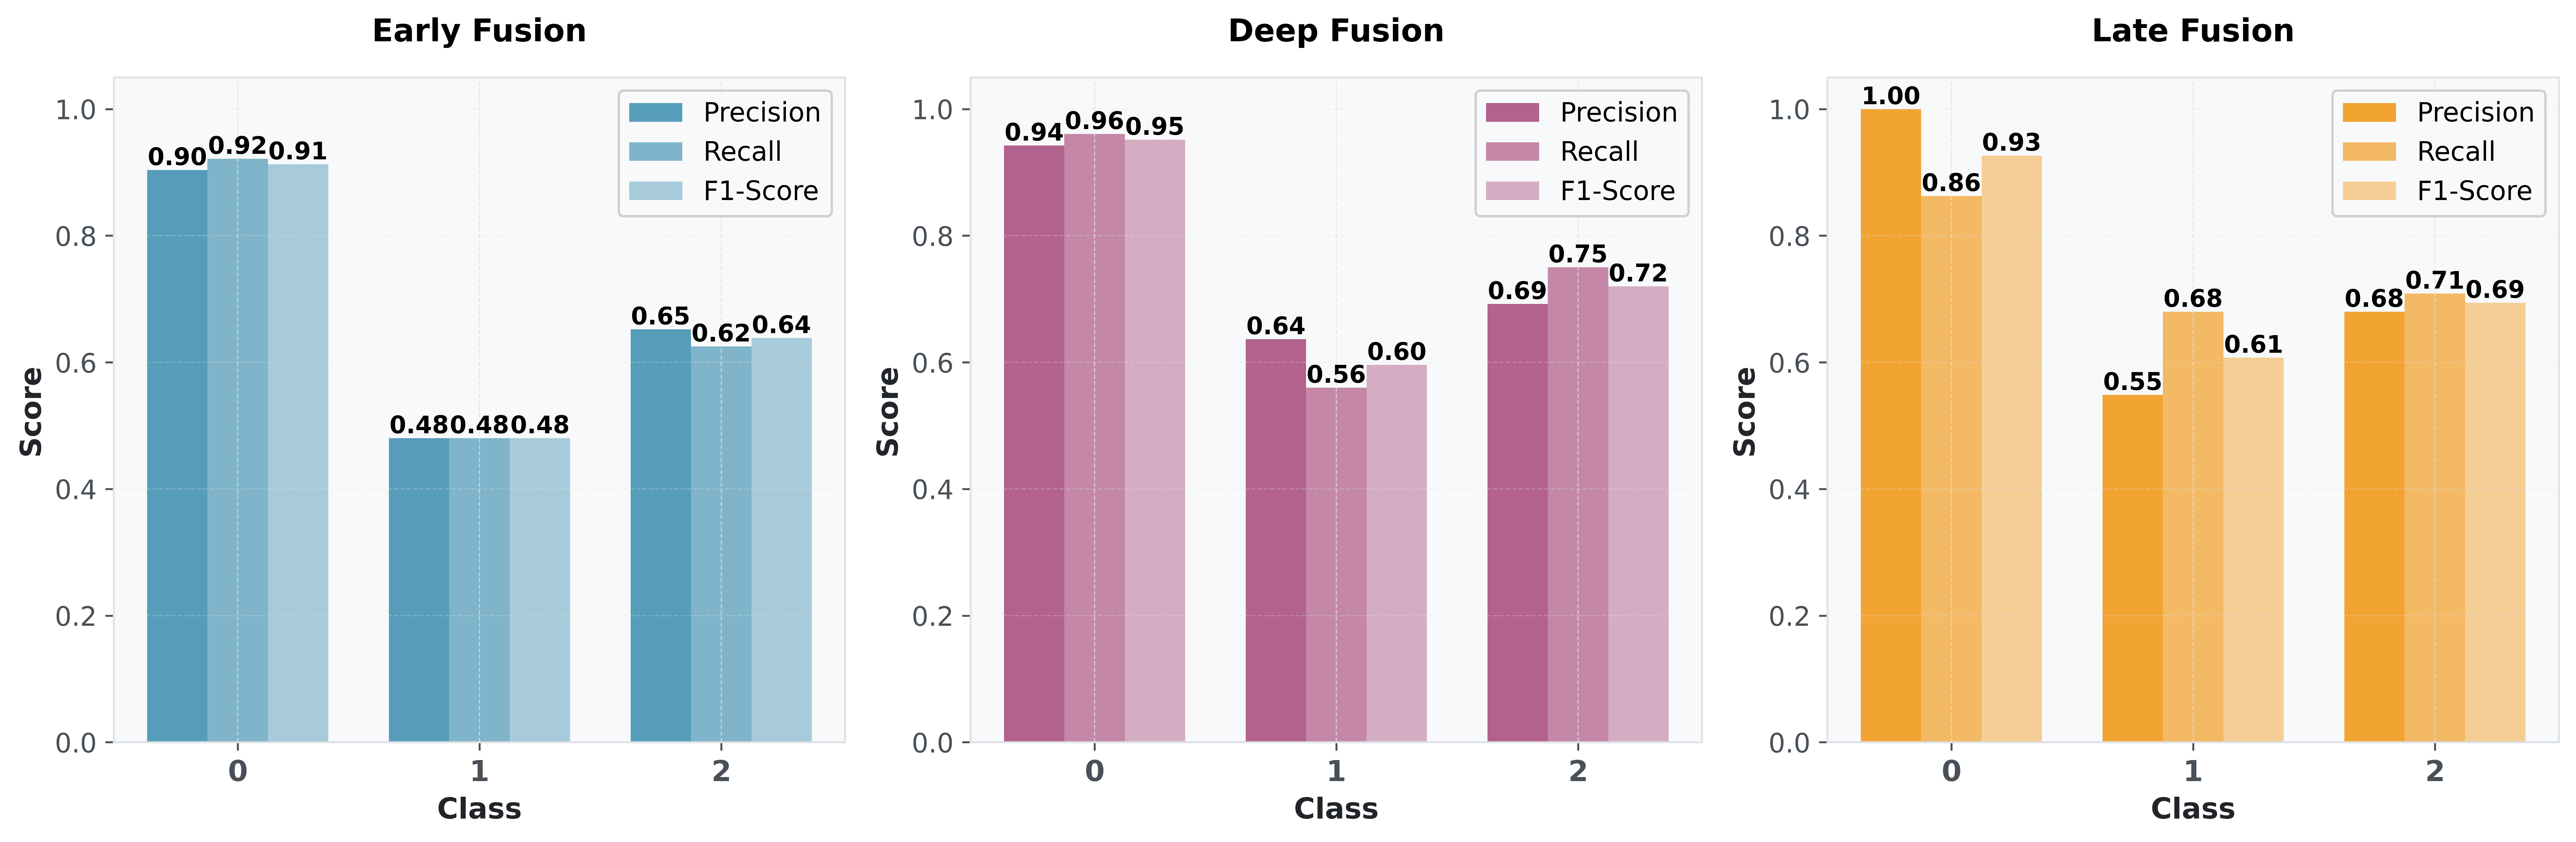
\includegraphics[width=1.0\textwidth]{images/multiclass_classwise_metrics.png}
    \caption{Class-wise precision, recall, and F1-scores for each fusion strategy under multiclass glaucoma grading.}
    \label{fig:multiclass_classwise_metrics}
\end{figure*}

Figure~\ref{fig:multiclass_roc_ovr} presents one-vs-rest (OvR) ROC curves for each glaucoma class across the three fusion strategies. For all models, class~0 (non-glaucoma) exhibits ROC curves closest to the ideal upper-left boundary, particularly for Deep and Late Fusion, indicating strong separability of normal cases. In contrast, class~1 (early glaucoma) shows more step-wise and irregular ROC behavior compared to class~2, reflecting higher uncertainty and overlap with adjacent severity levels. This observation aligns with the class-wise precision–recall trends, where intermediate-stage glaucoma remains the most challenging category. Overall, Deep Fusion achieves the most balanced OvR discrimination across classes, supporting its robustness for ordinal glaucoma grading.


\begin{figure*}[!t]
    \centering
    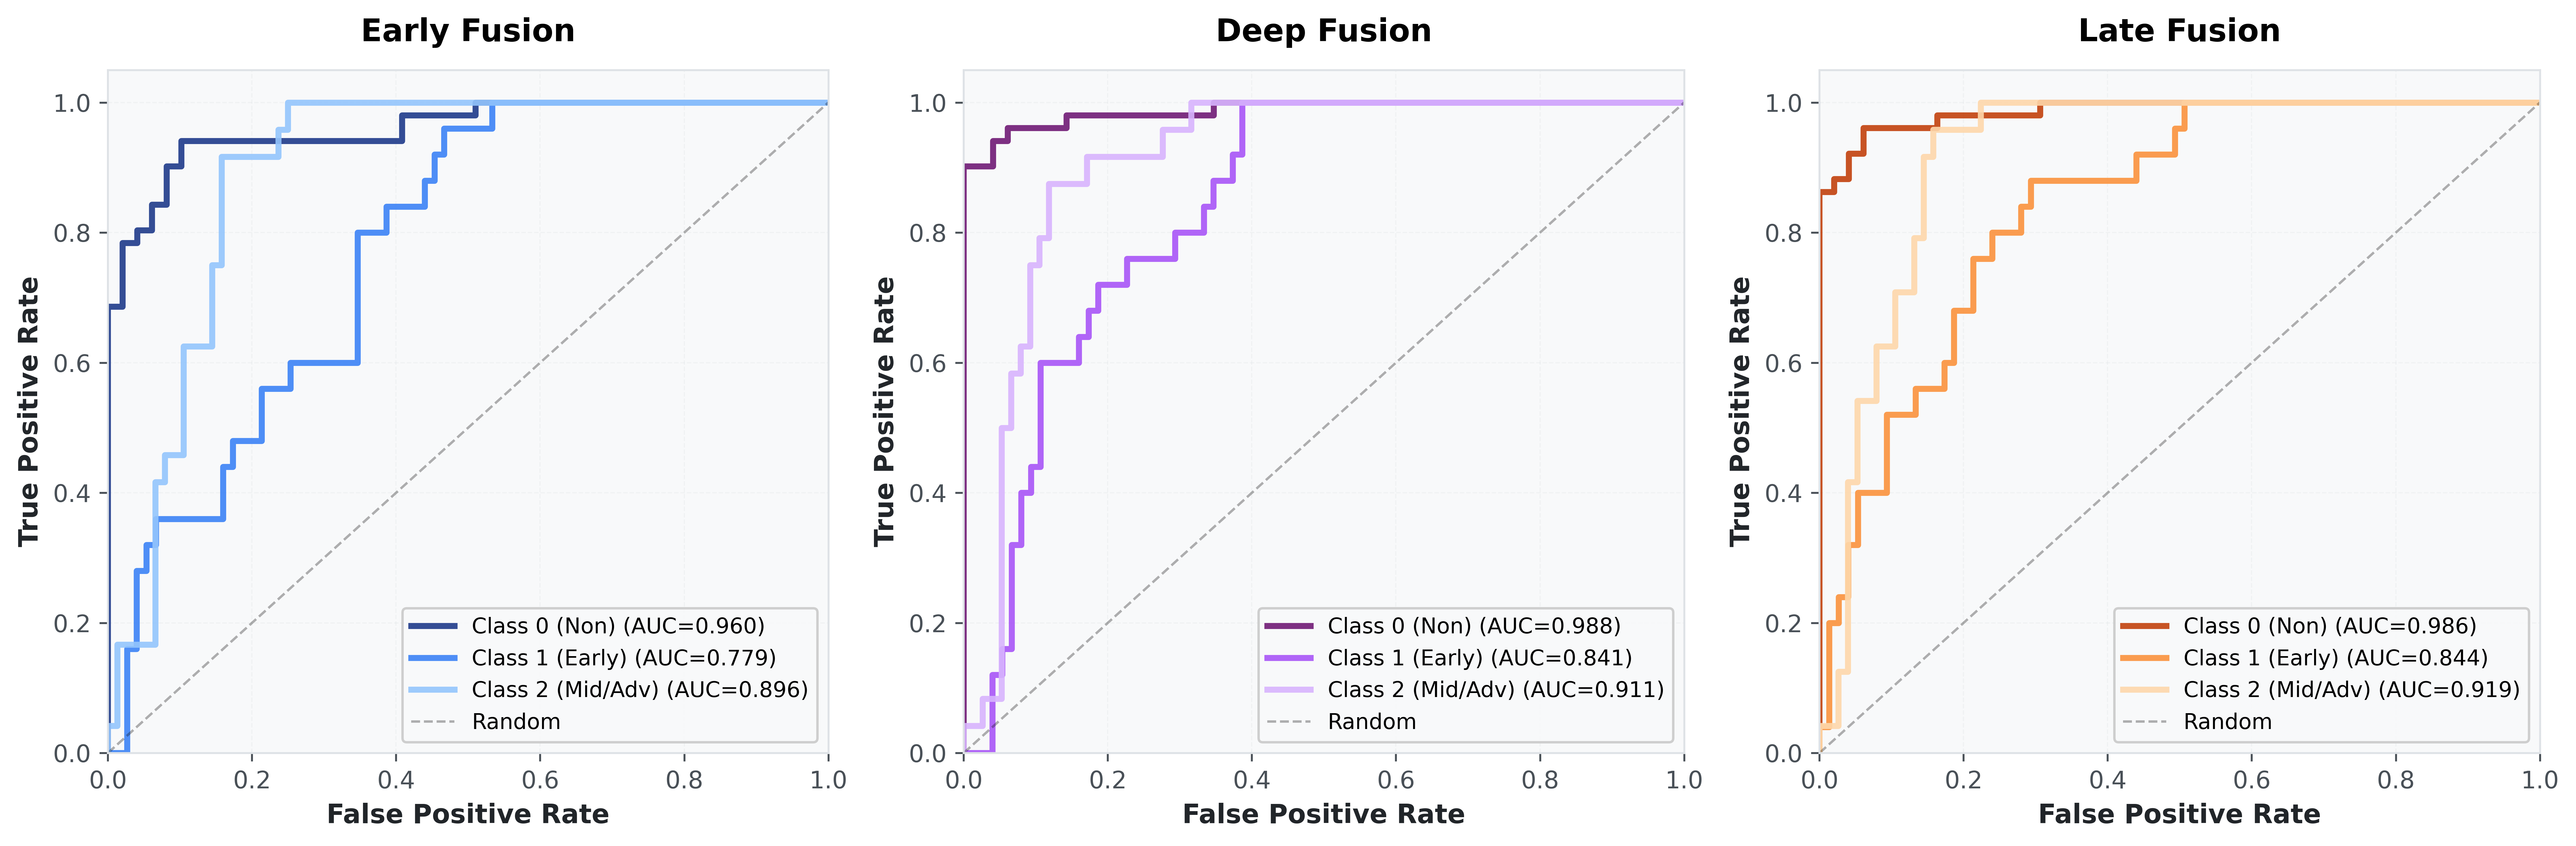
\includegraphics[width=1.0\textwidth]{images/multiclass_roc_ovr.png}
    \caption{One-vs-Rest ROC curves for each glaucoma class under multiclass grading for each fusion strategy.}
    \label{fig:multiclass_roc_ovr}
\end{figure*}

Finally, confusion matrices for multiclass grading are presented in Figure~\ref{fig:multiclass_confusion_matrices}. Deep Fusion achieves the highest number of correct predictions along the diagonal (49, 14, 18), indicating superior overall grading accuracy compared to Early Fusion (47, 12, 15) and Late Fusion (44, 17, 17). Misclassifications are predominantly concentrated between adjacent severity levels, particularly involving the intermediate (early glaucoma) class, which is expected due to overlapping structural characteristics across stages. Notably, Deep Fusion reduces confusion between neighboring classes more effectively than the other strategies, highlighting its ability to capture ordinal relationships and subtle severity transitions.

\begin{figure*}[!t]
    \centering
    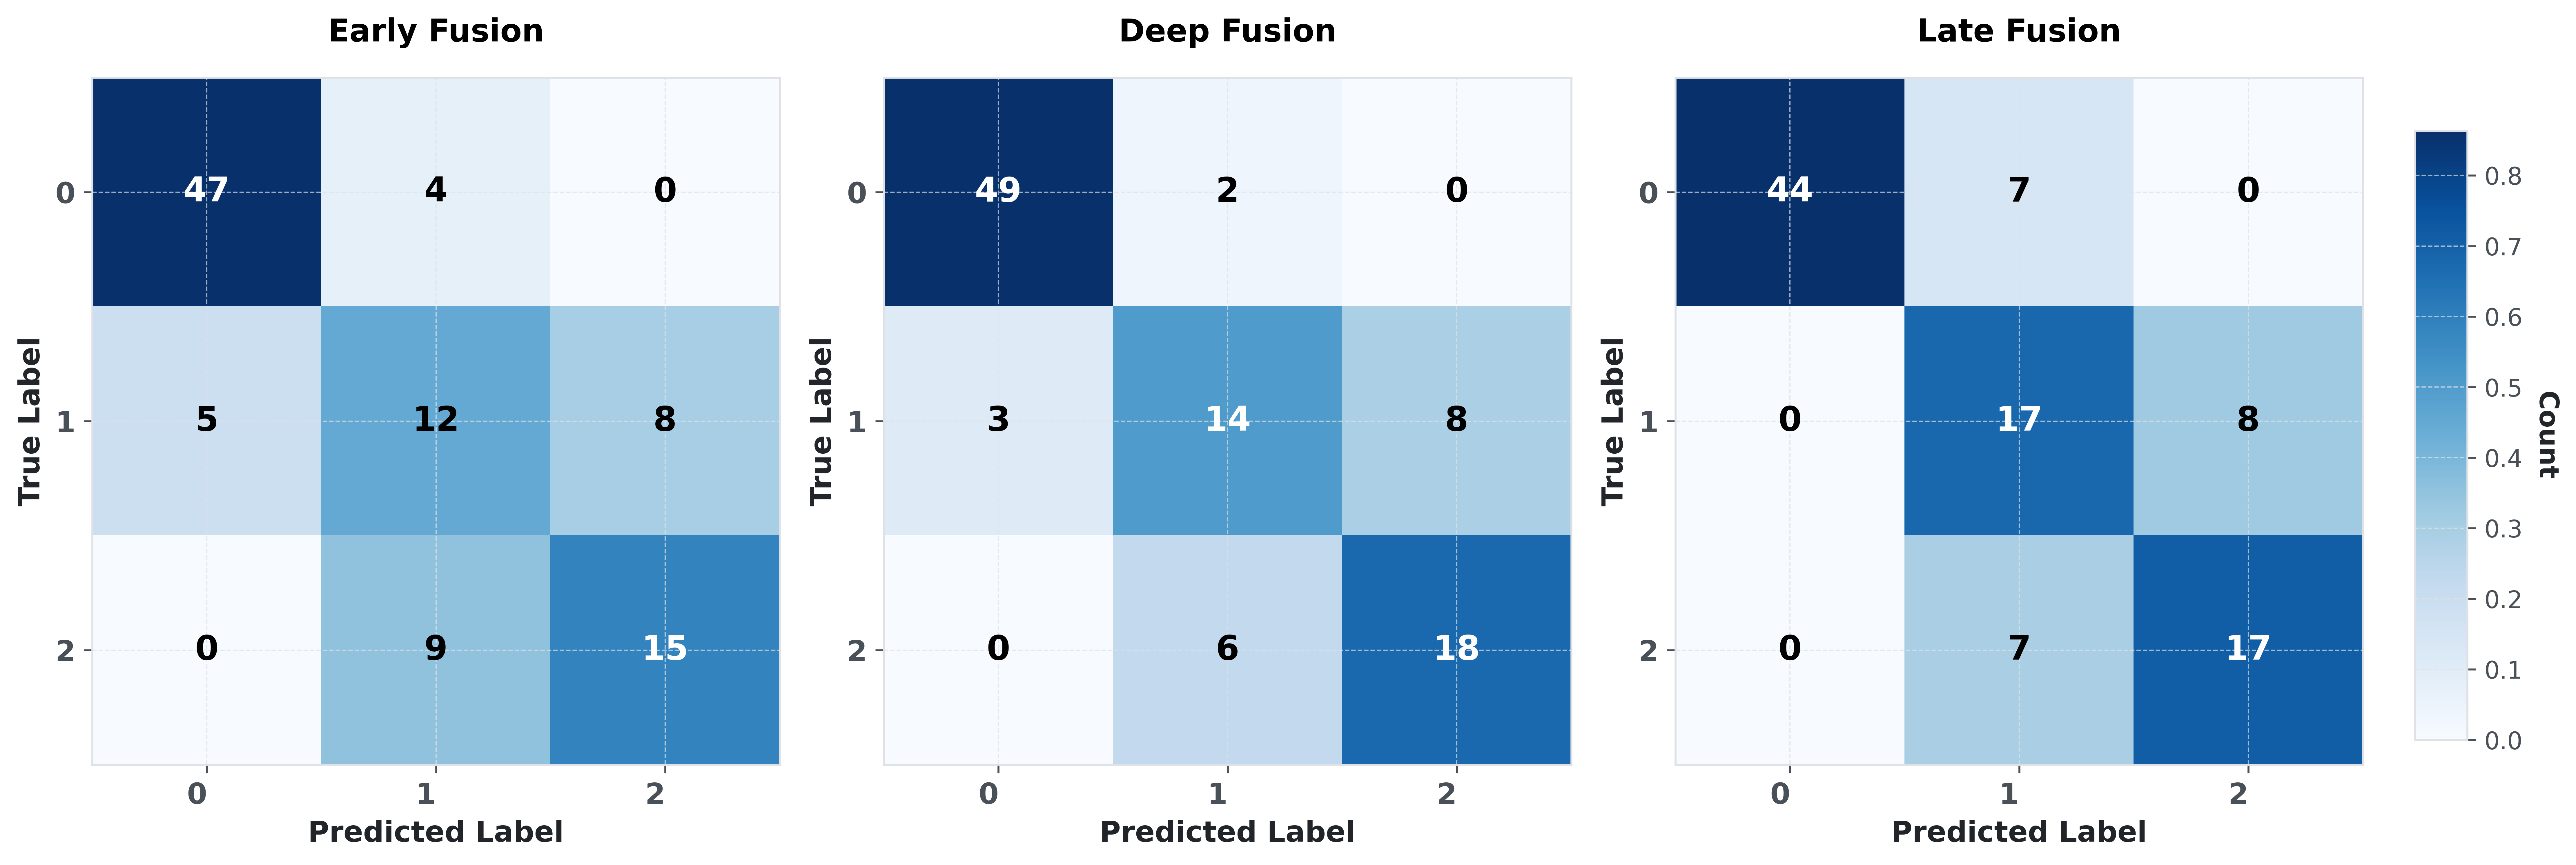
\includegraphics[width=0.9\textwidth]{images/multiclass_confusion_matrices.png}
    \caption{Confusion matrices for multiclass glaucoma grading under each fusion strategy.}
    \label{fig:multiclass_confusion_matrices}
\end{figure*}

\subsubsection{Five-Fold Cross-Validation Results}
\label{subsubsec:grading_cv}

To further evaluate the robustness of the proposed multimodal fusion strategies for multiclass glaucoma grading, five-fold cross-validation was conducted similar to glaucoma screening by merging the training and validation splits of the GAMMA dataset while preserving the original class distribution. The merged set of 200 samples was partitioned into five-folds, and each fusion strategy was trained and evaluated under identical training and calibration pipelines. The held-out test split remained unchanged to ensure consistency with the default evaluation protocol.

Table~\ref{tab:grading_cv_summary} summarizes the cross-validation performance across folds. Results are reported as mean $\pm$ standard deviation, with minimum and maximum values shown in brackets. Across all fusion strategies, the observed variability is relatively small, indicating stable performance under different training partitions. Deep Fusion achieves the highest agreement metric (QWK), suggesting improved capability in capturing ordinal severity relationships. Late Fusion demonstrates competitive macro-averaged metrics, indicating balanced class-wise performance, while Early Fusion maintains consistent results despite its simpler fusion formulation. The slightly lower mean performance observed in cross
validation compared to the single-split results is expected because hyperparameter tuning was performed on the default validation split, which may have introduced better
alignment with the test set distribution.

\begin{table*}[!t]
    \centering
    \caption{Five-fold cross-validation results for multiclass glaucoma grading (mean $\pm$ std [min, max]).}
    \label{tab:grading_cv_summary}
    \scriptsize
    \setlength{\tabcolsep}{6pt}
    \begin{tabular}{|l|c|c|c|}
        \hline
        \textbf{Metric}                & \textbf{Early Fusion} & \textbf{Deep Fusion} & \textbf{Late Fusion} \\
        \hline
        Accuracy                       &
        $0.720 \pm 0.021\,[0.68,0.74]$ &
        $0.752 \pm 0.019\,[0.72,0.78]$ &
        $0.752 \pm 0.035\,[0.69,0.79]$                                                                       \\

        Cohen's Kappa                  &
        $0.557 \pm 0.033\,[0.50,0.59]$ &
        $0.604 \pm 0.027\,[0.56,0.64]$ &
        $0.605 \pm 0.052\,[0.52,0.67]$                                                                       \\

        QWK                            &
        $0.762 \pm 0.026\,[0.72,0.80]$ &
        $0.820 \pm 0.021\,[0.77,0.84]$ &
        $0.788 \pm 0.045\,[0.70,0.83]$                                                                       \\

        Macro Precision                &
        $0.685 \pm 0.022\,[0.65,0.72]$ &
        $0.694 \pm 0.025\,[0.66,0.73]$ &
        $0.723 \pm 0.035\,[0.68,0.77]$                                                                       \\

        Macro Recall                   &
        $0.674 \pm 0.020\,[0.64,0.69]$ &
        $0.693 \pm 0.023\,[0.66,0.72]$ &
        $0.704 \pm 0.031\,[0.66,0.75]$                                                                       \\

        Macro F1-score                 &
        $0.671 \pm 0.018\,[0.64,0.69]$ &
        $0.689 \pm 0.024\,[0.65,0.72]$ &
        $0.703 \pm 0.032\,[0.65,0.74]$                                                                       \\

        Weighted F1-score              &
        $0.729 \pm 0.019\,[0.69,0.74]$ &
        $0.755 \pm 0.017\,[0.73,0.78]$ &
        $0.757 \pm 0.032\,[0.71,0.80]$                                                                       \\

        AUC-ROC (OvR)                  &
        $0.872 \pm 0.027\,[0.82,0.90]$ &
        $0.903 \pm 0.008\,[0.89,0.91]$ &
        $0.904 \pm 0.007\,[0.89,0.92]$                                                                       \\
        \hline
    \end{tabular}
\end{table*}

To visualize performance variability across folds, Figure~\ref{fig:grading_cv_boxplots} presents box plots for representative grading metrics including QWK, accuracy, and macro F1-score. The relatively narrow interquartile ranges across fusion strategies indicate stable behavior under different data partitions. Deep Fusion and Late Fusion demonstrate slightly higher median values with lower dispersion, suggesting stronger ordinal consistency and reduced sensitivity to fold composition.

\begin{figure*}[!t]
    \centering
    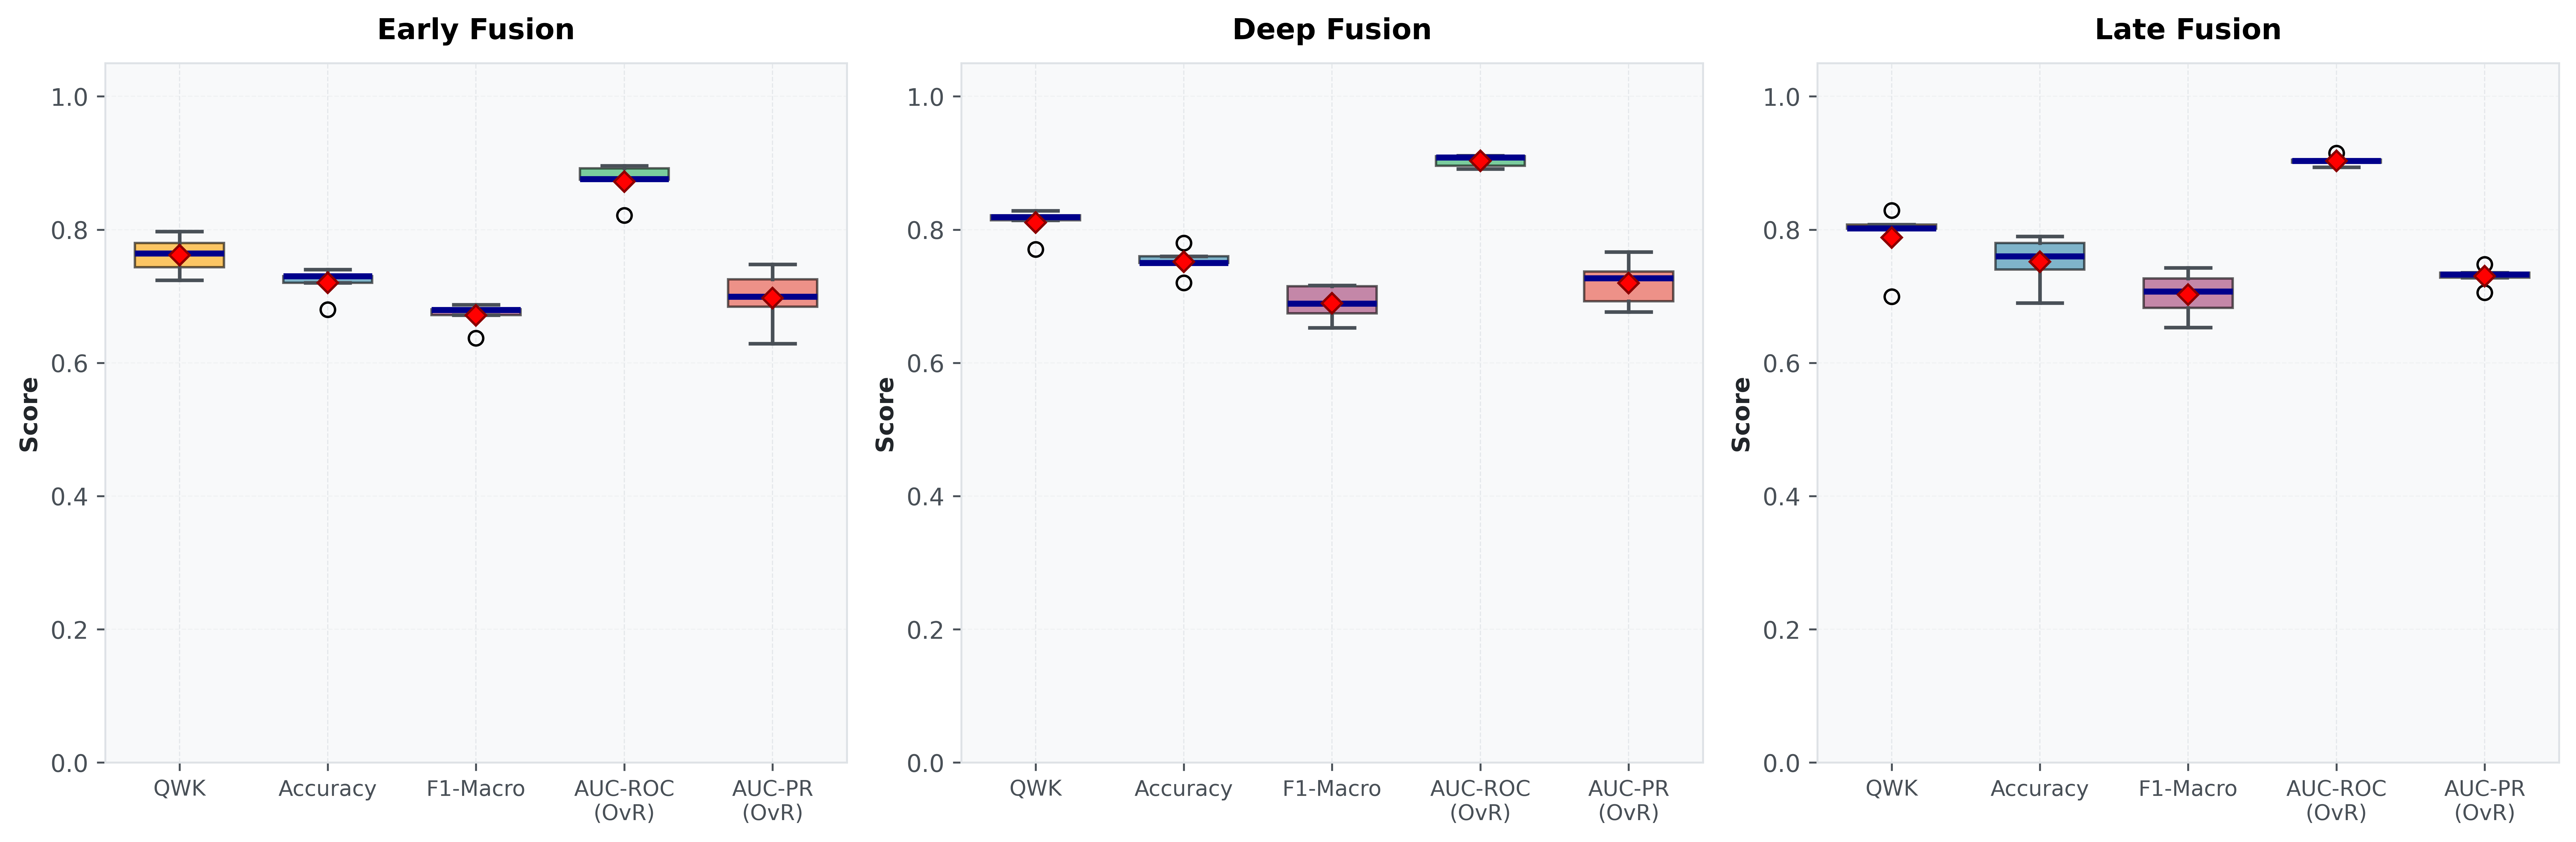
\includegraphics[width=\textwidth]{images/multiclass-cv-boxplots.png}
    \caption{Five-fold cross-validation: box plots metric distributions for multiclass glaucoma grading across fusion strategies.}
    \label{fig:grading_cv_boxplots}
\end{figure*}

To further examine class-level behavior, Figure~\ref{fig:grading_cv_confusion} shows the accumulated confusion matrices obtained by aggregating predictions across all folds. Most misclassifications occur between adjacent severity levels, particularly between early and mid-advanced glaucoma. Such behavior is expected due to the ordinal nature of glaucoma progression and the subtle structural differences between neighboring disease stages. Importantly, severe misclassifications across distant classes remain rare, especially for the Deep Fusion strategy, indicating clinically reasonable error patterns.

\begin{figure*}[!t]
    \centering
    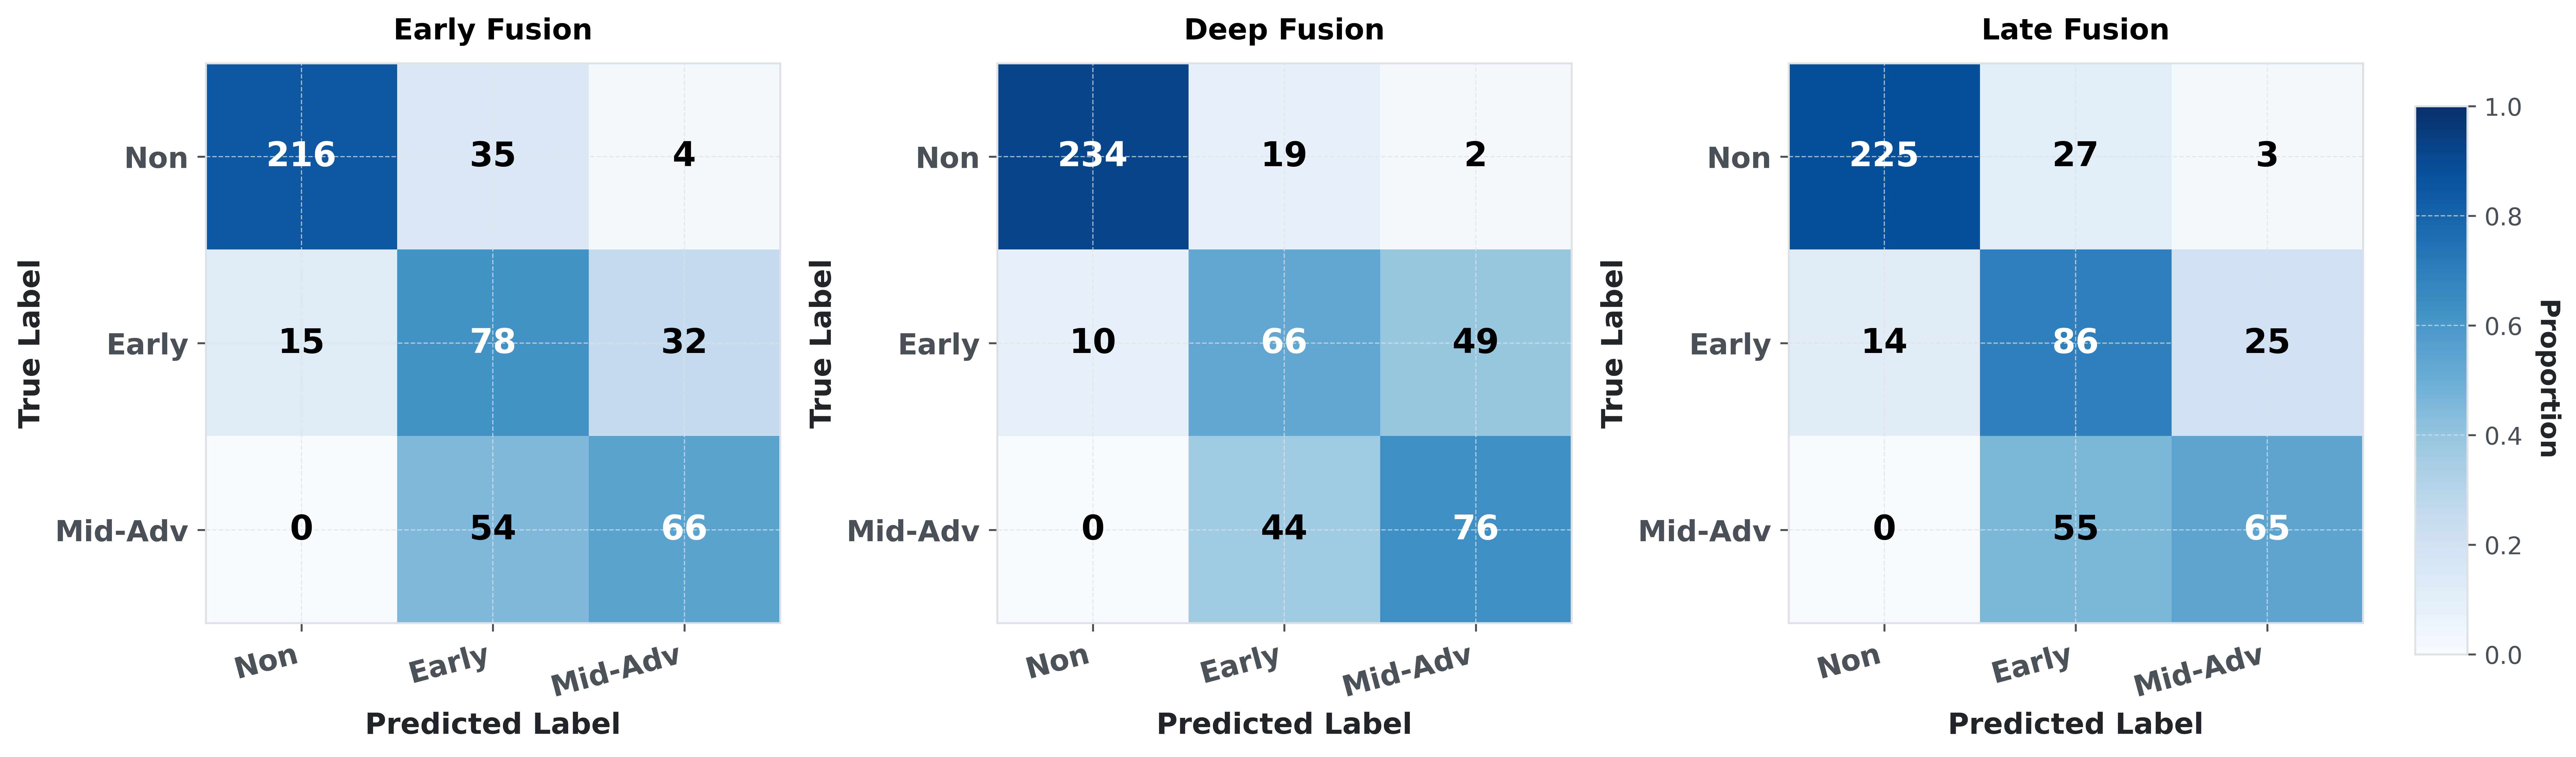
\includegraphics[width=\textwidth]{images/multiclass-cv-confusion-matrices.png}
    \caption{Five-fold cross-validation: Accumulated confusion matrices across folds for multiclass glaucoma grading.}
    \label{fig:grading_cv_confusion}
\end{figure*}

Overall, the cross-validation results confirm that the proposed multimodal framework maintains stable grading performance across different training partitions. This robustness suggests that the observed improvements are not artifacts of a particular data split but arise from the proposed fusion architectures and multimodal learning design.

\subsubsection{Bootstrapped Confidence Interval Results}
\label{subsubsec:multiclass_bootstrap}

To quantify predictive uncertainty and assess statistical robustness, we estimated confidence intervals for key multiclass metrics using non-parametric bootstrap resampling. A total of 1000 bootstrap samples were drawn from the test set with replacement, and 95\% confidence intervals were computed for each metric.

Table~\ref{tab:multiclass_bootstrap_ci} reports the bootstrap mean and standard deviation for accuracy, macro- and weighted-F1, macro-precision and recall, Cohen’s kappa, QWK, and OvR AUC-ROC across fusion strategies. Deep Fusion exhibits the highest mean QWK with comparatively low variance, indicating stable ordinal grading performance under resampling. Early and Late Fusion strategies also demonstrate consistent behavior, with overlapping confidence ranges that reflect competitive performance under uncertainty.

\begin{table*}[!t]
    \centering
    \caption{Bootstrapped performance estimates (1000 resamples, 95\% CI) for multiclass glaucoma grading. Values are reported as mean $\pm$ std [CI$_{95\%}$].}
    \label{tab:multiclass_bootstrap_ci}
    \scriptsize
    \setlength{\tabcolsep}{6pt}
    \begin{tabular}{|l|c|c|c|}
        \hline
        \textbf{Metric}                & \textbf{Early Fusion} & \textbf{Deep Fusion} & \textbf{Late Fusion} \\
        \hline
        Accuracy                       &
        $0.739 \pm 0.044$ [0.65, 0.82] &
        $0.809 \pm 0.039$ [0.73, 0.88] &
        $0.780 \pm 0.041$ [0.70, 0.86]                                                                       \\
        \hline
        F1-score (Macro)               &
        $0.674 \pm 0.049$ [0.58, 0.77] &
        $0.751 \pm 0.047$ [0.66, 0.84] &
        $0.739 \pm 0.046$ [0.65, 0.84]                                                                       \\
        \hline
        F1-score (Weighted)            &
        $0.738 \pm 0.046$ [0.65, 0.82] &
        $0.805 \pm 0.041$ [0.73, 0.88] &
        $0.791 \pm 0.038$ [0.72, 0.87]                                                                       \\
        \hline
        Precision (Macro)              &
        $0.679 \pm 0.050$ [0.58, 0.78] &
        $0.756 \pm 0.048$ [0.66, 0.85] &
        $0.743 \pm 0.043$ [0.66, 0.83]                                                                       \\
        \hline
        Recall (Macro)                 &
        $0.676 \pm 0.048$ [0.58, 0.77] &
        $0.756 \pm 0.046$ [0.66, 0.84] &
        $0.750 \pm 0.047$ [0.66, 0.84]                                                                       \\
        \hline
        Cohen’s Kappa                  &
        $0.576 \pm 0.066$ [0.45, 0.70] &
        $0.689 \pm 0.060$ [0.57, 0.80] &
        $0.653 \pm 0.061$ [0.54, 0.78]                                                                       \\
        \hline
        QWK                            &
        $0.804 \pm 0.035$ [0.73, 0.87] &
        $0.860 \pm 0.031$ [0.80, 0.92] &
        $0.833 \pm 0.033$ [0.77, 0.90]                                                                       \\
        \hline
        AUC-ROC (OvR)                  &
        $0.902 \pm 0.022$ [0.86, 0.94] &
        $0.938 \pm 0.017$ [0.90, 0.97] &
        $0.929 \pm 0.018$ [0.89, 0.96]                                                                       \\
        \hline
        AUC-ROC (Macro)                &
        $0.878 \pm 0.025$ [0.83, 0.92] &
        $0.913 \pm 0.021$ [0.87, 0.95] &
        $0.917 \pm 0.021$ [0.88, 0.96]                                                                       \\
        \hline
        AUC-PR (OvR)                   &
        $0.714 \pm 0.045$ [0.63, 0.81] &
        $0.740 \pm 0.046$ [0.66, 0.84] &
        $0.777 \pm 0.049$ [0.68, 0.87]                                                                       \\
        \hline
    \end{tabular}
\end{table*}


Figure~\ref{fig:multiclass_bootstrap_boxplots} visualizes the bootstrap distributions for selected representative metrics, including QWK, accuracy, macro-F1, OvR AUC-ROC, and OvR AUC-PR. The compact interquartile ranges observed across fusion strategies further support the robustness of the proposed framework, while reinforcing the advantage of Deep Fusion for glaucoma severity grading.

\begin{figure*}[!t]
    \centering
    
\includegraphics[width=1.0\textwidth]{images/multiclass_bootstrap_boxplots.png}
    \caption{Bootstrap distributions for selected multiclass grading metrics across fusion strategies: (a) QWK, (b) Accuracy, (c) Macro-F1, (d) OvR AUC-ROC, (e) OvR AUC-PR.}
    \label{fig:multiclass_bootstrap_boxplots}
\end{figure*}

Collectively, these results demonstrate that the proposed multimodal fusion framework supports reliable and uncertainty-aware multiclass glaucoma grading, complementing its strong performance in binary screening and enabling comprehensive clinical assessment within a unified architecture.


\subsection{EXPLAINABLE AI RESULTS}

Explainability analyses were conducted using Grad-CAM visualizations generated from models trained under the binary glaucoma screening protocol. This choice is justified because the core multimodal fusion architectures, attention mechanisms, and feature extraction backbones remain identical across both screening and grading tasks, with differences confined to the task-specific classifier heads and loss formulations. As Grad-CAM reflects spatial feature attribution within shared representation layers, the resulting visual explanations are representative of the learned multimodal attention patterns for both diagnostic objectives.

Grad-CAM visualizations were obtained for representative test set samples from each fusion strategy. Figure~\ref{fundus-xai} and Figure~\ref{oct-xai} illustrate the fundus and OCT explainability results, respectively, produced by the best-performing models of each fusion paradigm.

For fundus images, the Grad-CAM overlays consistently highlight clinically meaningful anatomical regions associated with glaucoma assessment. In particular, strong activations are frequently observed around the optic disc boundary, the neuroretinal rim, and adjacent peripapillary regions. These structures are routinely examined by ophthalmologists when evaluating glaucomatous changes, as alterations such as optic disc cupping, neuroretinal rim thinning, and peripapillary RNFL loss are established biomarkers of glaucoma. The alignment between the highlighted regions and these clinically recognized structures suggests that the multimodal models learn representations that correspond closely to the visual cues used in routine ophthalmic diagnosis.

\begin{figure}[!t]
    \centering
    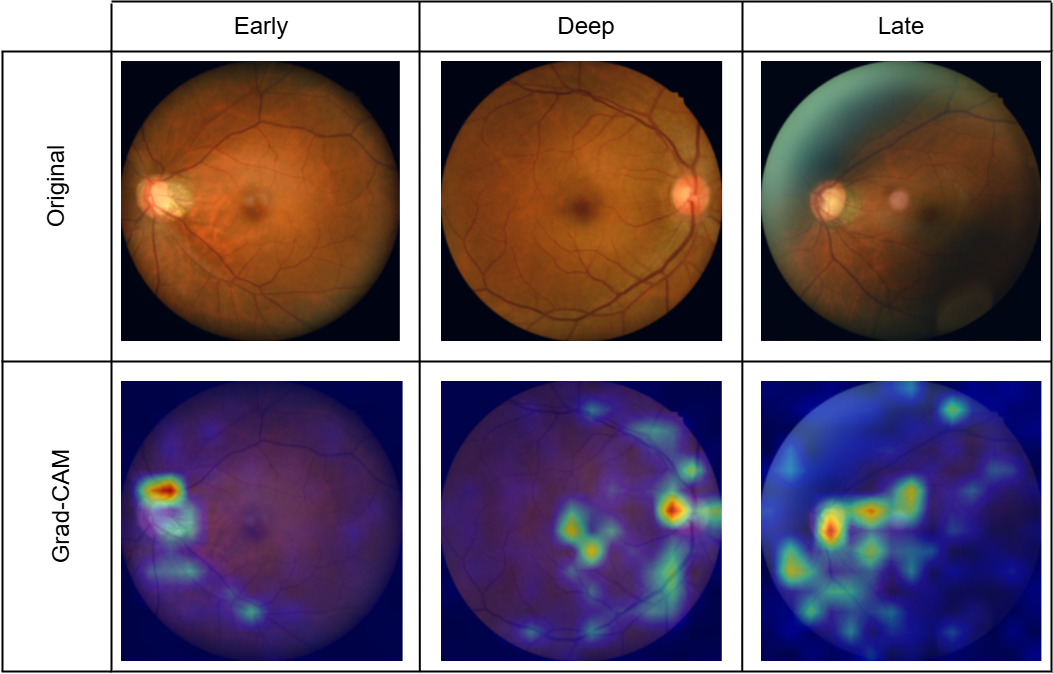
\includegraphics[width=1\columnwidth]{images/fundus-xai.png}
    \caption{Fundus Grad-CAM visualizations for representative test samples from each fusion strategy.}
    \label{fundus-xai}
\end{figure}

For the OCT modality, explainability follows a two-stage approach. First, the Multiple Instance Learning (MIL) attention mechanism identifies the most informative B-scans within each OCT volume. Based on these attention weights, the three highest-contributing slices per sample are selected for visualization. Grad-CAM is then applied at the slice level to localize salient intra-slice regions. As shown in Figure~\ref{oct-xai}, the highlighted areas frequently correspond to retinal layer structures, particularly regions associated with the retinal nerve fiber layer (RNFL) and adjacent inner retinal layers. Structural thinning and deformation of these layers are well-recognized indicators of glaucomatous damage. The model's focus on these areas therefore indicates that the learned features capture clinically relevant structural patterns present in OCT imaging.

\begin{figure}[!t]
    \centering
    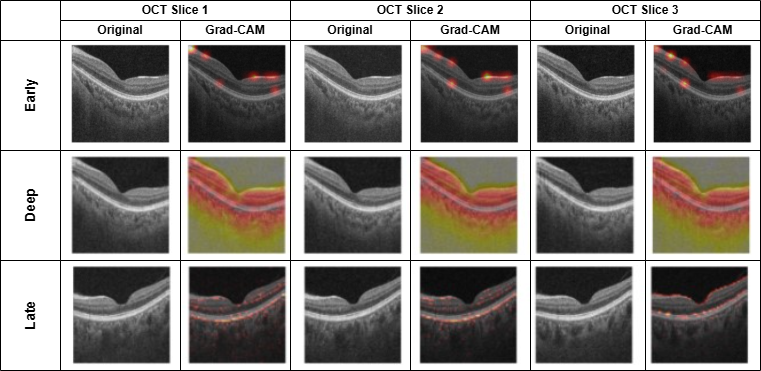
\includegraphics[width=1\columnwidth]{images/oct-xai.png}
    \caption{OCT Grad-CAM visualizations for representative test samples from each fusion strategy, showing three high-attention B-scans per model.}
    \label{oct-xai}
\end{figure}

Overall, the Grad-CAM visualizations demonstrate that the proposed multimodal fusion models base their predictions on anatomically meaningful structures in both fundus photographs and OCT scans. The consistent attention to clinically relevant regions such as the optic disc, neuroretinal rim, and retinal nerve fiber layer supports the interpretability of the learned representations and reinforces the potential of the framework as a clinically meaningful decision-support tool for glaucoma analysis.


\subsection{ABLATION STUDY}

We conducted ablation experiments to quantify the contribution of key architectural and preprocessing components in the proposed multimodal glaucoma screening framework. All ablations follow the default single data split protocol to ensure fair comparison across configurations and fusion strategies.
Importantly, these ablation results demonstrate that performance improvements are consistently associated with the proposed architectural components rather than specific hyperparameter configurations. Even under identical training settings, removing key modules such as the multimodal fusion mechanisms leads to noticeable performance degradation, confirming the architectural contribution of the proposed design.

\subsubsection{Glaucoma Screening (Binary) Ablation Analysis}

Table~\ref{tab:binary-ablation-condensed} summarizes the binary glaucoma screening ablation results. To maintain compactness, only Accuracy, AUC-ROC, Precision, and Recall are reported.

\begin{table*}[!t]
    \centering
    \caption{Condensed ablation results for binary glaucoma screening.}
    \label{tab:binary-ablation-condensed}
    \scriptsize
    \setlength{\tabcolsep}{3pt}
    \begin{tabular}{|l|cccc|cccc|cccc|}
        \hline
        \multirow{2}{*}{Configuration}     &
        \multicolumn{4}{c|}{Early Fusion}  &
        \multicolumn{4}{c|}{Deep Fusion}   &
        \multicolumn{4}{c|}{Late Fusion}                                \\
        \cline{2-13}
                                           & Acc  & AUC  & Prec & Rec &
        Acc                                & AUC  & Prec & Rec  &
        Acc                                & AUC  & Prec & Rec          \\
        \hline
        \textbf{No FiLM modulation}        &
        0.89                               & 0.96 & 0.84 & 0.96 &
        --                                 & --   & --   & --   &
        --                                 & --   & --   & --           \\
        \textbf{No cross-attn \& gating}   &
        --                                 & --   & --   & --   &
        0.95                               & 0.99 & 0.96 & 0.94 &
        --                                 & --   & --   & --           \\
        \textbf{No scaling \& conf. net.}  &
        --                                 & --   & --   & --   &
        --                                 & --   & --   & --   &
        0.94                               & 0.98 & 0.98 & 0.90         \\
        \hline
        \textbf{Fundus only}               &
        0.92                               & 0.97 & 0.90 & 0.94 &
        0.90                               & 0.96 & 0.92 & 0.88 &
        0.94                               & 0.97 & 0.94 & 0.94         \\
        \textbf{OCT only}                  &
        0.92                               & 0.97 & 0.89 & 0.96 &
        0.89                               & 0.94 & 0.87 & 0.92 &
        0.90                               & 0.96 & 0.92 & 0.88         \\
        \hline
        \textbf{No OCT-MIL}                &
        0.90                               & 0.97 & 0.90 & 0.90 &
        0.88                               & 0.95 & 0.89 & 0.86 &
        0.94                               & 0.99 & 0.89 & 1.00         \\
        \hline
        \textbf{No ROI cropping}           &
        0.89                               & 0.95 & 0.87 & 0.92 &
        0.92                               & 0.99 & 0.90 & 0.94 &
        0.96                               & 0.99 & 0.94 & 0.98         \\
        \hline
        \textbf{Selected model (baseline)} &
        0.92                               & 0.97 & 0.90 & 0.94 &
        0.95                               & 1.00 & 0.92 & 0.98 &
        0.95                               & 0.98 & 0.94 & 0.96         \\
        \hline
    \end{tabular}
\end{table*}

The ablation results confirm that each fusion-specific enhancement contributes positively to diagnostic performance. FiLM modulation improves Early Fusion by rebalancing modality dominance at the feature level, while cross-attention and gating strengthen Deep Fusion by enabling selective and context-aware cross-modal interaction. In Late Fusion, temperature scaling with confidence weighting enhances decision reliability through improved calibration. The ablation experiment of evaluating the impact of attention-based OCT slice aggregation demonstrates Early Fusion is particularly sensitive to the absence of OCT-MIL, while Deep and Late Fusion exhibit mixed behavior, reflecting differing reliance on early volumetric integration. In addition, ROI cropping consistently yields performance gains across fusion strategies by suppressing non-informative background regions and geometric deformations, allowing the models to focus on clinically relevant retinal structures. Across all strategies, multimodal configurations consistently outperform unimodal baselines, validating the complementary nature of fundus and OCT information for glaucoma screening.


\subsubsection{Glaucoma Grading (Multiclass) Ablation Analysis}

To assess the contribution of architectural components and preprocessing choices under the multiclass glaucoma grading protocol, we conducted a parallel set of ablation experiments using the default single-split evaluation. Consistent with the grading objective, we report Accuracy, Quadratically Weighted Cohen’s Kappa (QWK), Macro F1-score, and AUC-ROC (one-vs-rest), which jointly capture ordinal agreement, class-balanced performance, and ranking quality.

Table~\ref{tab:multiclass-ablation-condensed} summarizes the multiclass ablation results in a condensed format aligned with the binary screening ablations.

\begin{table*}[!t]
    \centering
    \caption{Condensed ablation results for multiclass glaucoma grading.}
    \label{tab:multiclass-ablation-condensed}
    \scriptsize
    \setlength{\tabcolsep}{3pt}
    \begin{tabular}{|l|cccc|cccc|cccc|}
        \hline
        \multirow{2}{*}{Configuration}     &
        \multicolumn{4}{c|}{Early Fusion}  &
        \multicolumn{4}{c|}{Deep Fusion}   &
        \multicolumn{4}{c|}{Late Fusion}                                \\
        \cline{2-13}
                                           & Acc  & Qwk  & F1   & AUC &
        Acc                                & Qwk  & F1   & AUC  &
        Acc                                & Qwk  & F1   & AUC          \\
        \hline
        \textbf{No FiLM modulation}        &
        0.76                               & 0.80 & 0.71 & 0.89 &
        --                                 & --   & --   & --   &
        --                                 & --   & --   & --           \\
        \textbf{With cross-attn \& gating} &
        --                                 & --   & --   & --   &
        0.80                               & 0.85 & 0.75 & 0.92 &
        --                                 & --   & --   & --           \\
        \textbf{No scaling \& conf. net.}  &
        --                                 & --   & --   & --   &
        --                                 & --   & --   & --   &
        0.74                               & 0.78 & 0.67 & 0.92         \\
        \hline
        \textbf{Fundus only}               &
        0.67                               & 0.70 & 0.60 & 0.89 &
        0.75                               & 0.80 & 0.70 & 0.88 &
        0.76                               & 0.81 & 0.73 & 0.89         \\
        \textbf{OCT only}                  &
        0.66                               & 0.65 & 0.60 & 0.86 &
        0.66                               & 0.67 & 0.49 & 0.87 &
        0.63                               & 0.69 & 0.61 & 0.85         \\
        \hline
        \textbf{No OCT-MIL}                &
        0.73                               & 0.80 & 0.66 & 0.88 &
        0.74                               & 0.80 & 0.67 & 0.90 &
        0.78                               & 0.84 & 0.73 & 0.92         \\
        \hline
        \textbf{No ROI cropping}           &
        0.75                               & 0.80 & 0.69 & 0.90 &
        0.80                               & 0.85 & 0.75 & 0.93 &
        0.74                               & 0.78 & 0.68 & 0.91         \\
        \hline
        \textbf{Selected model (baseline)} &
        0.74                               & 0.81 & 0.68 & 0.88 &
        0.81                               & 0.86 & 0.76 & 0.91 &
        0.78                               & 0.84 & 0.74 & 0.92         \\
        \hline
    \end{tabular}
\end{table*}

Across the evaluated configurations, multimodal models generally outperform or remain competitive with unimodal baselines, confirming the complementary value of fundus photographs and OCT volumes for glaucoma severity grading. Architectural enhancements exhibit clear task-dependent behavior. FiLM modulation improves Early Fusion by facilitating modality-aware feature rebalancing, whereas optional multi-head cross-attention and gating modules slightly degrade Deep Fusion performance under multiclass learning. This degradation is attributed to increased architectural complexity and the introduction of gating and CLS-token interactions, which can attenuate discriminative information and introduce noise when modeling fine-grained three-class decision boundaries under limited data. In contrast, removing confidence-aware scaling in Late Fusion leads to degraded ordinal agreement, highlighting the importance of calibrated decision-level fusion for severity grading. Overall, the simplified Deep Fusion configuration achieves the most stable and effective grading performance, consistent with its superior QWK observed in the primary results.

The OCT-MIL ablation demonstrates that attention-based slice aggregation plays a critical role in constructing informative volumetric representations by preserving discriminative structural cues. For glaucoma grading, removal of OCT-MIL consistently degrades performance, confirming its importance under class imbalance and ordinal severity modeling severity grading protocol.

\subsection{Failure Case Analysis}
\label{subsec:failure_analysis}

Although the proposed multimodal framework achieves strong performance for both glaucoma screening and grading, examining misclassified samples provides useful insight into model limitations and the inherent difficulty of automated glaucoma diagnosis.

For multiclass grading, the accumulated cross-validation confusion matrices show that most errors occur between adjacent severity classes rather than between clinically distant categories. Based on the aggregated grading predictions, adjacent-class errors account for 97.1\%, 98.4\%, and 97.6\% of all errors for Early, Deep, and Late Fusion, respectively. This indicates that the models rarely confuse normal eyes directly with mid-advanced glaucoma; instead, most mistakes occur around the clinically ambiguous boundaries between normal and early glaucoma or between early and mid-advanced glaucoma. Such behaviour is consistent with the ordinal nature of glaucoma progression and suggests clinically reasonable failure patterns.

Qualitative inspection of prediction errors reveals three recurring categories. First, some normal eyes exhibit physiologically large optic cups that visually resemble glaucomatous cupping in fundus photographs, occasionally leading to false-positive predictions. Such cases are also challenging in clinical practice, where distinguishing physiological cupping from early glaucomatous damage may require careful assessment of OCT structure and longitudinal change.

Second, some errors are associated with OCT image artifacts or degraded scan quality. Motion artifacts, truncated retinal boundaries, incomplete layer visibility, or low-contrast B-scans can reduce the reliability of structural features extracted from OCT volumes. When such slices receive high OCT-MIL attention, they may disproportionately influence the final prediction.

Third, early-stage glaucoma remains the most challenging category because structural changes may be subtle and overlap with normal anatomical variation. In these borderline cases, both fundus images and OCT scans may exhibit only mild deviations from healthy anatomy, limiting the discriminative cues available to the model. These observations reinforce the need to interpret automated predictions alongside clinical expertise, particularly for borderline early glaucoma, physiological cupping, and cases with OCT quality degradation.

\section{DISCUSSION}

\subsection{Principal Findings}

This study presents a unified multimodal learning framework for automated glaucoma analysis that supports both binary glaucoma screening and multiclass glaucoma severity grading within a single architectural paradigm. Unlike many prior studies that focus on a single fusion mechanism or diagnostic objective, the proposed framework systematically evaluates three complementary multimodal fusion strategies—Early, Deep, and Late Fusion—spanning integration from pixel-level interaction to latent feature fusion and decision-level combination. A key characteristic of the framework is its transformer-centric design, with optional hybrid backbones such as CoAtNet selected through hyperparameter optimization. Both fundus photographs and OCT volumes are processed using vision transformer encoders, demonstrating that transformer-based representations can effectively capture complex retinal structural patterns in multimodal ophthalmic imaging. The architecture is modular and backbone-agnostic, allowing different transformer variants to be incorporated within a consistent multimodal pipeline.

Experimental results demonstrate that transformer-based multimodal learning can achieve strong and stable diagnostic performance even under limited-data conditions. For binary glaucoma screening, the Deep Fusion configuration achieved an AUC-ROC of 0.995 together with high sensitivity and accuracy on the held-out test set, indicating excellent discrimination between glaucomatous and non-glaucomatous eyes. Robustness was further confirmed through five-fold cross-validation, where all fusion strategies maintained strong performance with relatively low variance across folds. For multiclass glaucoma grading, the Deep Fusion strategy achieved a quadratically weighted Cohen’s kappa (QWK) of 0.8633 together with competitive accuracy and macro-F1 scores, indicating strong agreement with ordinal severity labels. Importantly, grading reliability was further quantified using both cross-validation and bootstrap-based confidence interval estimation, providing statistically grounded performance estimates beyond single-split evaluation. Such uncertainty-aware evaluation remains relatively underexplored in glaucoma grading studies but is particularly valuable for clinical decision-support applications.

Table~\ref{tab:summary_results} provides a consolidated overview of the best-performing results for both screening and grading tasks. The results consistently favor Deep Fusion, while also demonstrating that Early and Late Fusion offer competitive alternatives depending on the desired level of multimodal interaction. The superior performance of Deep Fusion suggests that intermediate latent-space integration provides an effective balance between preserving modality-specific representations and enabling cross-modal feature interaction.
Clinically, fundus photographs and OCT volumes provide complementary but non-isomorphic evidence: fundus images capture optic disc cupping, neuroretinal rim morphology, vascular context, and peripapillary appearance, whereas OCT captures cross-sectional retinal layer structure, including RNFL and GCIPL-related changes. Pixel-level fusion may combine modalities before each has formed a stable anatomical representation, while decision-level fusion delays interaction until after modality-specific predictions have already been formed. Deep Fusion allows each modality to first encode its own anatomical evidence and then interact in a shared latent space, which likely explains its stronger screening sensitivity and higher ordinal agreement for grading.

Several complementary factors likely contribute to the strong performance of the proposed framework. First, multimodal fusion integrates global contextual information from fundus photographs with detailed structural cues from OCT volumes, providing a richer representation of glaucomatous changes than either modality alone. Clinically relevant abnormalities may appear both in optic disc and neuroretinal rim morphology in fundus images and in layer-specific structural alterations captured by OCT. Second, the consistent performance across fusion strategies highlights the suitability of transformer-based representations for multimodal ophthalmic imaging. Unlike convolutional architectures with progressively expanding receptive fields, transformers capture global contextual relationships through self-attention, enabling interactions between distant retinal regions. This capability is particularly beneficial for modeling structural indicators such as optic disc morphology, neuroretinal rim thinning, and retinal nerve fiber layer changes, while also facilitating cross-modal alignment between heterogeneous modalities.

Third, the OCT-MIL aggregation module improves volumetric OCT representation by emphasizing diagnostically informative B-scan slices and reducing the influence of less relevant signals. Since glaucoma-related structural changes are not uniformly distributed across OCT volumes, slice-level aggregation helps focus learning on the most informative regions. Finally, the strong performance is supported not only by architectural design but also by carefully aligned optimization strategies. Despite being trained exclusively on the relatively small-scale GAMMA dataset, the proposed models achieved robust performance without relying on external multimodal cohorts or glaucoma-specific pretraining. Targeted data augmentation, label smoothing, differential learning rates, regularization, and extensive hyperparameter optimization enabled stable training under limited-data conditions.

Taken together, these results demonstrate that the proposed framework offers more than task-specific predictive performance. A single transformer-based multimodal architecture can jointly support glaucoma screening and severity grading while providing a controlled platform for studying how different levels of multimodal interaction influence clinical prediction. This combination of unified task support, systematic fusion analysis, and competitive performance represents a central contribution of the present work.

\begin{table}[!t]
    \centering
    \caption{Best-performing results of the proposed fusion strategies for glaucoma screening and grading on the GAMMA dataset.}
    \label{tab:summary_results}
    \scriptsize
    \setlength{\tabcolsep}{5pt}
    \begin{tabular}{lcccc}
        \hline
        \multirow{2}{*}{\textbf{Fusion Strategy}}
                     & \multicolumn{2}{c}{\textbf{Screening (Binary)}}
                     & \multicolumn{2}{c}{\textbf{Grading (Multiclass)}}                                                       \\
        \cline{2-5}
                     & \textbf{AUC-ROC}                                  & \textbf{Acc.}   & \textbf{Acc.}   & \textbf{QWK}    \\
        \hline
        Early Fusion & 0.9743                                            & 0.9200          & 0.7400          & 0.8065          \\
        Deep Fusion  & \textbf{0.9952}                                   & \textbf{0.9500} & \textbf{0.8100} & \textbf{0.8633} \\
        Late Fusion  & 0.9835                                            & 0.9500          & 0.7800          & 0.8355          \\
        \hline
    \end{tabular}
\end{table}


\subsection{Comparison with Prior Work}

Table~\ref{tab:gamma_comparison} situates the proposed methods within the broader context of recent GAMMA-based glaucoma grading studies. In the multiclass grading setting, the proposed Deep Fusion model achieves competitive performance relative to several established multimodal approaches and exceeds or matches representative benchmark levels reported in a number of prior studies. At the same time, these comparisons should be interpreted in light of differing methodological objectives. While several recent methods are specifically optimized for glaucoma grading, the proposed framework is designed as a unified multimodal architecture capable of supporting both glaucoma screening and severity grading within a consistent training and evaluation pipeline. This broader design objective allows systematic investigation of multimodal fusion strategies while maintaining competitive diagnostic performance across tasks.

Notably, some task-specific grading architectures, such as M2F3, report higher peak grading performance. However, these methods are primarily tailored to maximize accuracy on the multiclass grading task itself. In contrast, the present study emphasizes architectural generality, robustness, and interpretability by unifying screening and grading tasks, supporting multiple fusion paradigms, and incorporating post-hoc calibration together with uncertainty-aware evaluation. From this perspective, the contribution of the proposed framework lies not only in achieving strong grading performance, but also in offering a more flexible and extensible design for multimodal glaucoma analysis. Such a framework is valuable because it supports comparative analysis across multiple fusion granularities and provides a reusable foundation that can be adapted as transformer-based vision architectures continue to evolve.

An important point in interpreting these comparisons is that direct benchmarking for binary glaucoma screening on GAMMA remains limited, as most published GAMMA-based studies formulate the problem as multiclass severity grading rather than binary diagnostic screening. Consequently, the binary results reported in this study primarily demonstrate the feasibility, robustness, and clinical promise of the proposed framework rather than superiority over an established set of GAMMA-based binary baselines. Nevertheless, the very high AUC-ROC and sensitivity observed for screening indicate that the unified framework is highly effective in distinguishing glaucomatous from non-glaucomatous cases and may therefore be well suited to screening-oriented clinical applications.

These comparisons highlight an important distinction between the proposed framework and many existing GAMMA-based approaches. Rather than optimizing a single architecture for one benchmark task, this study develops a consistent multimodal pipeline through which multiple fusion strategies can be systematically analyzed under a common transformer-based setting. This allows performance differences to be interpreted more directly in terms of fusion behavior rather than confounding architectural differences. In this sense, the proposed framework contributes methodological value in addition to competitive predictive performance. Even where certain task-specific models report slightly higher peak results, the present work offers additional advantages in terms of architectural transparency, modularity, generality across tasks, and explicit robustness assessment.


\begin{table*}[!t]
    \centering
    \caption{Comparison with prior work on the GAMMA dataset for multiclass glaucoma grading.}
    \label{tab:gamma_comparison}
    \scriptsize
    \setlength{\tabcolsep}{5pt}
    \resizebox{\textwidth}{!}{%
        \begin{tabular}{|p{0.22\textwidth}|p{0.16\textwidth}|c|c|p{0.30\textwidth}|}
            \hline
            \textbf{Method} & \textbf{Modalities}                                & \textbf{Accuracy} & \textbf{Kappa / QWK}   & \textbf{Remarks} \\
            \hline
            GAMMA Challenge Best (SmartDSP)~\cite{wu2023gamma}
                            & Fundus + OCT                                       & --                & 0.8549 (QWK)
                            & Top-ranked GAMMA challenge submission.                                                                             \\
            \hline
            GAMMA Challenge Top-3 (Avg.)~\cite{wu2023gamma}
                            & Fundus + OCT                                       & --                & $\sim$0.84--0.85 (QWK)
                            & Representative performance of leading teams.                                                                       \\
            \hline
            MOD-Net~\cite{wang2025dual}
                            & Fundus + OCT                                       & $\sim$0.75        & --
                            & CNN-based multimodal fusion.                                                                                       \\
            \hline
            COROLLA~\cite{cai2022corolla}
                            & Fundus + OCT                                       & $\sim$0.90        & $\sim$0.855
                            & Ordinal-aware multimodal grading.                                                                                  \\
            \hline
            GeCoM-Net~\cite{wang2024geometric}
                            & Fundus + OCT                                       & --                & 0.8840
                            & Geometry-guided multimodal alignment.                                                                              \\
            \hline
            M2F3~\cite{zhao2025enhancing}
                            & Fundus + OCT                                       & \textbf{0.9400}   & \textbf{0.9015}
                            & Multi-stage fusion with peak grading performance.                                                                  \\
            \hline\hline
            \textbf{Ours -- Early Fusion}
                            & Fundus + OCT                                       & 0.7400            & 0.8065 (QWK)
                            & Pixel-level fusion with FiLM modulation.                                                                           \\
            \hline
            \textbf{Ours -- Deep Fusion}
                            & Fundus + OCT                                       & \textbf{0.8100}   & \textbf{0.8633} (QWK)
                            & Task-aligned latent fusion with strong robustness.                                                                 \\
            \hline
            \textbf{Ours -- Late Fusion}
                            & Fundus + OCT                                       & 0.7800            & 0.8355 (QWK)
                            & Confidence-calibrated decision-level fusion.                                                                       \\
            \hline
        \end{tabular}}
\end{table*}


\subsection{Methodological Insights and Explainability}

The ablation studies provide further insight into the methodological contributions of this work. By systematically isolating the impact of fusion-specific enhancements, modality contributions, and preprocessing choices, the experiments show that strong performance does not arise solely from the availability of multiple modalities, but also from how cross-modal information is structured and integrated. Components such as spatial normalization, FiLM-based feature modulation, cross-modal interaction design, and confidence-aware fusion play important roles in improving multimodal representation learning. These findings reinforce the view that successful multimodal glaucoma analysis depends not only on combining fundus and OCT information, but on designing fusion mechanisms that are well aligned with the heterogeneity of ophthalmic imaging data.

The unified implementation of Early, Deep, and Late Fusion within a common transformer-based framework also strengthens the interpretability of the comparative analysis itself. Because all three fusion strategies are evaluated under broadly consistent backbone and training conditions, the relative performance differences can be attributed more confidently to the level and mechanism of multimodal interaction rather than to unrelated architectural confounds. This makes the fusion comparison more meaningful and improves reproducibility. In this regard, the framework serves not only as a predictive model but also as an experimental platform for understanding how different multimodal integration strategies behave in glaucoma screening and grading settings.

Explainability is another key strength of the study. Grad-CAM visualizations across fundus images and attention-weighted OCT slice analyses consistently highlight clinically relevant anatomical regions, including the optic nerve head, retinal nerve fiber layer, and macular structures. The alignment between model attention and known ophthalmic biomarkers supports clinical trust and provides qualitative evidence that the models base their predictions on meaningful retinal features rather than predominantly on spurious correlations or irrelevant image regions. This is particularly important in the context of clinical decision support, where transparency and plausibility are central to adoption. Although post-hoc explanation methods do not by themselves establish causal validity, the observed agreement between highlighted regions and clinically meaningful structures strengthens confidence in the biological plausibility of the learned representations.

\subsection{Limitations and Generalizability}

Despite these strengths, several limitations should be acknowledged. First, all experiments were conducted on the publicly available GAMMA dataset, which provides paired fundus photographs and volumetric OCT scans with clinically annotated glaucoma severity labels. While GAMMA is one of the few benchmarks supporting multimodal glaucoma analysis, reliance on a single dataset limits the ability to fully assess cross-dataset generalization. Dataset-specific characteristics—including imaging devices, acquisition protocols, patient demographics, annotation practices, and disease prevalence—may influence the reported performance.

To mitigate potential overfitting to dataset-specific characteristics, several strategies were incorporated into the training pipeline, including strong data augmentation, regularization techniques, transformer backbones adapted for relatively small datasets, and stratified cross-validation for both screening and grading protocols. Together with bootstrap-based uncertainty estimation for grading results, these measures help promote stable learning and reduce sensitivity to individual data partitions. However, they cannot replace validation on independent clinical cohorts. External evaluation across different institutions, imaging devices, and patient populations remains necessary to determine whether the framework generalizes reliably beyond the conditions represented by GAMMA.

Second, although transformer-based models demonstrated strong performance in this study, stable convergence under limited-data medical imaging conditions still requires careful optimization and training strategies. The favorable results should therefore be interpreted as reflecting the interaction between architectural design and disciplined training procedures rather than implying that transformer models are universally straightforward to deploy.

Additional factors may affect real-world applicability. Variability in OCT scan quality, motion artifacts, segmentation inconsistencies, and other acquisition-related degradations may influence the reliability of extracted structural features. Demographic or site-specific biases within training data may also affect performance across underrepresented populations. Moreover, the framework assumes the availability of both fundus and OCT imaging together with consistent preprocessing and spatial normalization. While reasonable in controlled datasets such as GAMMA, real-world deployment may require mechanisms to handle missing modalities, heterogeneous devices, and non-standardized image quality.

Another limitation is that this study does not include a direct CNN-based multimodal comparator trained under the same experimental pipeline. Consequently, the results should not be interpreted as definitive evidence that transformer-based fusion is universally superior to convolutional alternatives. Instead, the findings demonstrate that transformer-centric multimodal fusion can achieve strong and robust performance for paired fundus–OCT glaucoma analysis, while comparative evaluation of transformer and CNN multimodal designs remains an important direction for future work.

Finally, although post-hoc calibration and uncertainty estimation were incorporated to improve prediction reliability, prospective clinical validation remains necessary to assess real-world utility. Clinical usefulness depends not only on predictive performance but also on workflow integration, robustness to distribution shift, interpretability, error tolerance, and reliable operation under practical conditions.

\subsection{Future Directions}

Several directions emerge from the findings of this study. First, external validation on larger, more diverse, and multi-center multimodal ophthalmic cohorts will be essential to assess generalizability across different imaging devices, acquisition settings, and patient populations. Second, the framework can be extended to incorporate additional clinically relevant modalities, such as visual field measurements, retinal nerve fiber layer thickness maps, or structured clinical metadata, moving toward a more comprehensive decision-support system for glaucoma management.

Given the consistent superiority of the Deep Fusion strategy across both screening and grading tasks, future work should particularly prioritize refined latent-space fusion architectures with improved task alignment, cross-modal interaction modeling, calibration, and robustness. Motivated by the performance trends observed in this study and in related multimodal glaucoma literature, further investigation of Deep Fusion may provide the most promising path toward improved multimodal representation learning under clinically realistic conditions. At the same time, handling missing modalities and heterogeneous imaging conditions remains a critical requirement for real-world deployment and should be addressed explicitly in future model design.

Another important direction involves explainable AI. Although the present study demonstrates promising qualitative alignment between learned attention patterns and clinically meaningful retinal structures, more clinically grounded explanation methods are needed to better characterize cross-modal decision mechanisms. Integrating explanation techniques with clinician-informed evaluation protocols may improve error analysis, strengthen trust, and support translational adoption.

Overall, this study establishes a robust, interpretable, and extensible transformer-based foundation for multimodal glaucoma analysis. By jointly supporting glaucoma screening and severity grading, systematically comparing Early, Deep, and Late fusion strategies, and incorporating robustness- and uncertainty-aware evaluation, the proposed framework contributes both methodological and practical value toward reliable AI-assisted ophthalmic diagnosis.

\section{CONCLUSION}

This work presented a unified transformer-based multimodal framework for glaucoma screening and glaucoma grading by integrating color fundus photographs and 3D OCT volumes through systematically designed Early, Deep, and Late Fusion strategies. By examining fusion at pixel, latent, and decision levels within a consistent experimental setting, the study provides a comprehensive analysis of how fusion granularity, architectural design, and task alignment influence diagnostic performance in multimodal ophthalmic learning.

Across both diagnostic protocols, the proposed models demonstrated strong and reliable performance on the GAMMA dataset despite limited sample size and class imbalance. In particular, the Deep Fusion architecture produced the most consistent results, combining high discriminative performance, robust calibration, and stable generalization. For glaucoma screening, the model achieved an AUC of 99.5\% with high sensitivity and minimal false negatives, while for glaucoma grading it delivered competitive accuracy and quadratically weighted kappa scores with narrow bootstrap confidence intervals. These results highlight the effectiveness of transformer-based latent fusion for aligning heterogeneous 2D fundus and 3D OCT representations.

The study further shows that task-aligned architectural design and lightweight enhancement modules—including FiLM-based modulation, cross-modal attention, gated rebalancing, and confidence-aware branch-wise scaling—contribute meaningfully to performance improvements, as confirmed through ablation analyses. All models were developed within a transformer-centric design space, primarily using vision transformer backbones and, where selected by optimization, compact hybrid architectures. Training exclusively on the GAMMA dataset suggests that transformer-driven multimodal learning can remain effective under carefully regularized low-data regimes, although external validation is required to confirm generalizability across devices, institutions, and patient populations. Explainability analyses using Grad-CAM and MIL attention further produced anatomically coherent visualizations, supporting the clinical plausibility of the learned representations.

Although further validation on larger multi-center cohorts is necessary to establish clinical readiness, this work provides a principled and extensible foundation for multimodal glaucoma analysis. By unifying glaucoma screening and grading within a single modular framework and systematically evaluating fusion strategies, robustness, calibration, and interpretability, the study advances the development of multimodal ophthalmic AI. Future work will focus on external clinical validation, integration of additional diagnostic modalities, and prospective evaluation toward real-world clinical decision-support systems.


%% If you have bib database file and want bibtex to generate the
%% bibitems, please use
%%
\bibliographystyle{elsarticle-num}
\bibliography{references}

%% else use the following coding to input the bibitems directly in the
%% TeX file.

%% Refer following link for more details about bibliography and citations.
%% https://en.wikibooks.org/wiki/LaTeX/Bibliography_Management

% % \begin{thebibliography}{00}

% % %% For numbered reference style
% % %% \bibitem{label}
% % %% Text of bibliographic item

% % \bibitem{lamport94}
% %   Leslie Lamport,
% %   \textit{\LaTeX: a document preparation system},
% %   Addison Wesley, Massachusetts,
% %   2nd edition,
% %   1994.

% % \end{thebibliography}
\end{document}

\endinput
%%
%% End of file `elsarticle-template-num.tex'.
